
\documentclass{article} \usepackage{iclr2024_conference,times}

\input{math_commands.tex}

\usepackage{hyperref}
\usepackage{url}
\usepackage{graphicx} 
\usepackage[most]{tcolorbox}
\usepackage{multirow}
\usepackage{multicol}
\usepackage{array}
\usepackage[usestackEOL]{stackengine}
\usepackage{booktabs}
\usepackage{wrapfig}
\usepackage{subcaption}
\usepackage{xspace}

\newcommand{\hide}[1]{}
\newcommand{\model}{CogVideoX\xspace}
\newcommand{\dong}[1]{\textbf{\color{red}[(Dong: #1 )]}}

\newtcolorbox{promptbox}[1][]{
  breakable,
  title=#1,
  colback=gray!5,
  colframe=black,
  colbacktitle=gray!15,
  coltitle=black,
  fonttitle=\bfseries,
  bottomrule=1.5pt,
  toprule=1.5pt,
  leftrule=1pt,
  rightrule=1pt,
  arc=0pt,
  outer arc=0pt,
  enhanced,
  before upper={\parindent=1.5em} }

\lstset{
  basicstyle=\ttfamily,
  breaklines=true,
  breakatwhitespace=false,
  columns=flexible,
  keepspaces=true,
  showspaces=false,
  showstringspaces=false,
  showtabs=false,
  tabsize=4,
  xleftmargin=0pt,
  xrightmargin=0pt
}

\newcommand{\aspace}{\hspace{1em}}


\title{

\includegraphics[width=0.3\textwidth]{images/logo.png}
A Text-to-Video Diffusion Model with Expert Transformer}




\author{Zhuoyi Yang*\aspace Jiayan Teng* \aspace Wendi Zheng\aspace Ming Ding\aspace Shiyu Huang \aspace Jiazheng Xu \aspace \\
\textbf{Yuanming Yang \aspace Xiaohan Zhang \aspace Xiaotao Gu 
\aspace Guanyu Feng \aspace  Da Yin \aspace Wenyi Hong \aspace } \\
\textbf{ Weihan Wang \aspace Yean Cheng \aspace Yuxuan Zhang \aspace Ting Liu \aspace Bin Xu \aspace Yuxiao Dong \aspace Jie Tang} \\
$^1$Zhipu AI\ \ \ \ \ \ $^2$Tsinghua University \\
\href{https://github.com/THUDM/CogVideo}{https://github.com/THUDM/CogVideo}
}

 
\newcommand{\fix}{\marginpar{FIX}}
\newcommand{\new}{\marginpar{NEW}}

\iclrfinalcopy \begin{document}


\maketitle

\renewcommand{\thefootnote}{}
\footnotetext{*equal contributions. Core contributors: Zhuoyi, Jiayan, Wendi, Ming, and Shiyu.}
\footnotetext{{\{yangzy22,tengjy20\}@mails.tsinghua.edu.cn, \{yuxiaod,jietang\}@tsinghua.edu.cn}}
\renewcommand{\thefootnote}{\arabic{footnote}}
\begin{abstract}
We introduce CogVideoX, a large diffusion transformer model capable of generating videos conditioned on text prompts. It applies a 3D VAE and a 3D transformer based on Expert Adaptive LayerNorm. Employing a progressive training technique, the model is able to generate coherent long-duration videos characterized by significant motion. Additionally, we propose a complete large-scale data processing pipeline, including various data cleaning strategies and video re-caption method, resulting in better generation quality and improved semantic alignment. Finally, CogVideoX achieves state-of-the-art performance across multiple machine metrics and human evaluations.
\end{abstract}

\section{Introduction}

The rapid development of text-to-video models has been phenomenal, driven by both the Transformer architecture~\cite{vaswani2017attention} and diffusion model~\cite{ho2020denoising}. 
Early attempts to pretrain and scale Transformers to generate videos from text have shown great promise, such as CogVideo~\cite{hong2022cogvideo} and Phenaki~\cite{villegas2022phenaki}. 
Meanwhile, diffusion models have recently made exciting advancements in multimodal generation, including video generation~\cite{singer2022make, ho2022imagen}. 
By using Transformers as the backbone of diffusion models, i.e., Diffusion Transformers (DiT) \cite{peebles2023scalable}, text-to-video generation has reached groundbreaking levels, as evidenced by the impressive Sora showcases~\cite{sora}.  


Despite these rapid advancements in DiTs, it remains technically unclear how to achieve long-term consistent video generation. 
Challenges such as efficiently modeling video data, effectively aligning videos with text semantics, as well as constructing the high-quality text-video pairs for model training have thus far been largely unaddressed. 


In this work, we train and introduce \model, a set of large-scale diffusion transformer models designed for generating long-term, temporally consistent videos. 
We address the challenges mentioned above by developing a 3D variational Autoencoder (VAE), an expert Transformer, and a video data filtering and captioning pipeline, respectively. 
First, to efficiently consume video data, we design and train a 3D causal VAE that compresses the video along both spatial and temporal dimensions. 
Compared to unfolding a video into a one-dimensional sequence in the pixel space, this strategy helps significantly reduce the sequence length and associated training compute. 
Unlike previous video models~\cite{blattmann2023stable} that often use a 2D VAE to encode each frame separately, the 3D VAE helps prevent flicker in the generated videos, that is, ensuring continuity among frames. 





\begin{figure}
\centering
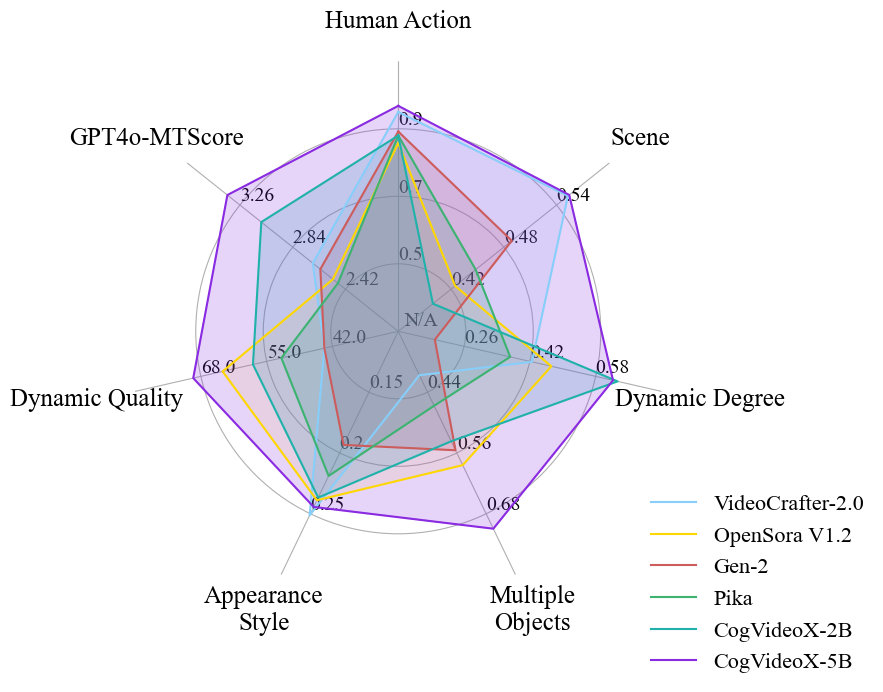
\includegraphics[width=0.7\linewidth]{images/bench_eval9.png}
\caption{The performance of openly-accessible text-to-video models in different aspects.}
\label{fig:radar}


\end{figure}



Second, to improve the alignment between videos and texts, we propose an expert Transformer with  expert adaptive LayerNorm to facilitate the fusion between the two modalities. 
To ensure the temporal consistency in video generation and  capture large-scale motions, we propose to use 3D full attention to comprehensively model the video along both temporal and spatial dimensions. 

Third, as most video data available online lacks accurate textual descriptions, we develop a video captioning pipeline capable of accurately describing video content. 
This pipeline is used to generate new textual descriptions for all video data, which significantly enhances \model's ability to grasp precise semantic understanding. 


In addition, we adopt and design progressive training techniques, including mixed-duration training and resolution progressive training, to further enhance the generation performance and stability of \model. Furthermore, we propose Explicit Uniform Sampling, which stablizes the training loss curve and accelerates convergence by setting different timestep sampling intervals on each data parallel rank.

Both machine and human evaluations suggest that \model outperforms well-known public models. 
Figure \ref{fig:radar} shows the performance of \model in different aspects. 

\model is an ongoing attempt to advance text-to-video generation. 
To facilitate further developments, we open-source the model weight of part of \model and the 3D VAE, and we plan to release future and larger models as well. 
Now open-sourced \model is capable of generating 720$\times$480 videos of six seconds with eight frames per second. 
It can be publicly accessed from \url{https://github.com/THUDM/CogVideo}. 


 







\hide{

\section{Introduction}

In recent years, diffusion models have made groundbreaking advancements in multimodal generation, such as image, video, speech and 3D generation. Among these, video generation is a rapidly evolving field and being extensively explored. Given the successful experiences with Large Language Models (LLMs), comprehensive scaling up of data volume, training iterations, and model size consistently enhances model performance. Additionally, there is more mature scaling experience with transformers compared to UNet. And DiT \cite{peebles2023scalable} has shown that transformers can effectively replace UNet as the backbone of diffusion models. Thus, transformer is a better choice for video generation.
However, long-term consistent video generation remains a significant challenge.  

The first challenge is that constructing a web-scale video data pipeline is considerably more difficult than for textual data. Video data is extremely diverse in distribution, quality varies greatly, and simple rule-based filtering is often insufficient for effective data selection. Consequently, processing video data is both time-consuming and highly complex.
There are numerous meaningless unrealistic videos, such as poor-quality edits and computer screen recordings. And many videos are difficult to watch normally, such as those with excessively shaky cameras. These types of data are harmful to the generative model's ability to learn genuine dynamic information. They need to be meticulously processed and filtered out to ensure the quality of the training dataset.

Additionally, most video data available online lacks accurate textual descriptions, significantly limiting the model's ability to grasp precise semantic understanding. To address this issue, we trained a video understanding model capable of accurately describing video content. We use it to generate new textual descriptions for all video data. 
To advance the field of video generation, we have decided to open-source this description model.

The high training cost is another significant challenge. If the video is unfolded into a one-dimensional sequence in the pixel space, the length would be extraordinarily long. To keep the computational cost within a feasible range, we trained a 3D VAE that compresses the video along both spatial and temporal dimensions. Additionally,  unlike previous video models that use a 2D VAE to encode each frame separately, 3D VAE ensures continuity among frames so that the generated videos do not flicker. 

Moreover, to improve the alignment between videos and texts, we propose an expert transformer to facilitate the interaction between the two modalities. Then, to ensure the consistency of video generation and to capture large-scale motions, it is necessary to comprehensively model the video along both temporal and spatial dimensions. Therefore, we opt for 3D full attention, as detailed in Section~\ref{sec:expert-transformer}.



} \section{The \model Architecture}\label{sec:model}


In the section, we present the \model model. 
Figure \ref{fig:model} illustrates the overall architecture. 
Given a pair of video and text input,  we design a \textbf{3D causal VAE} to compress the video into the latent space, and the latents are then patchified and unfolded into a long sequence denoted as $z_{\text{vision}}$. 
Simultaneously, we encode the textual input into text embeddings $z_{\text{text}}$ using T5~\cite{raffel2020exploring}. 
Subsequently, $z_{\text{text}}$ and $z_{\text{vision}}$ are concatenated along the sequence dimension. 
The concatenated embeddings are then fed into a stack of \textbf{expert transformer} blocks.
Finally, the model output are unpatchified to restore the original latent shape, which is then decoded using a 3D causal VAE decoder to reconstruct the video. 
We illustrate the technical design of the 3D causal VAE and expert transfomer in detail.


\begin{figure}[h]
\begin{center}
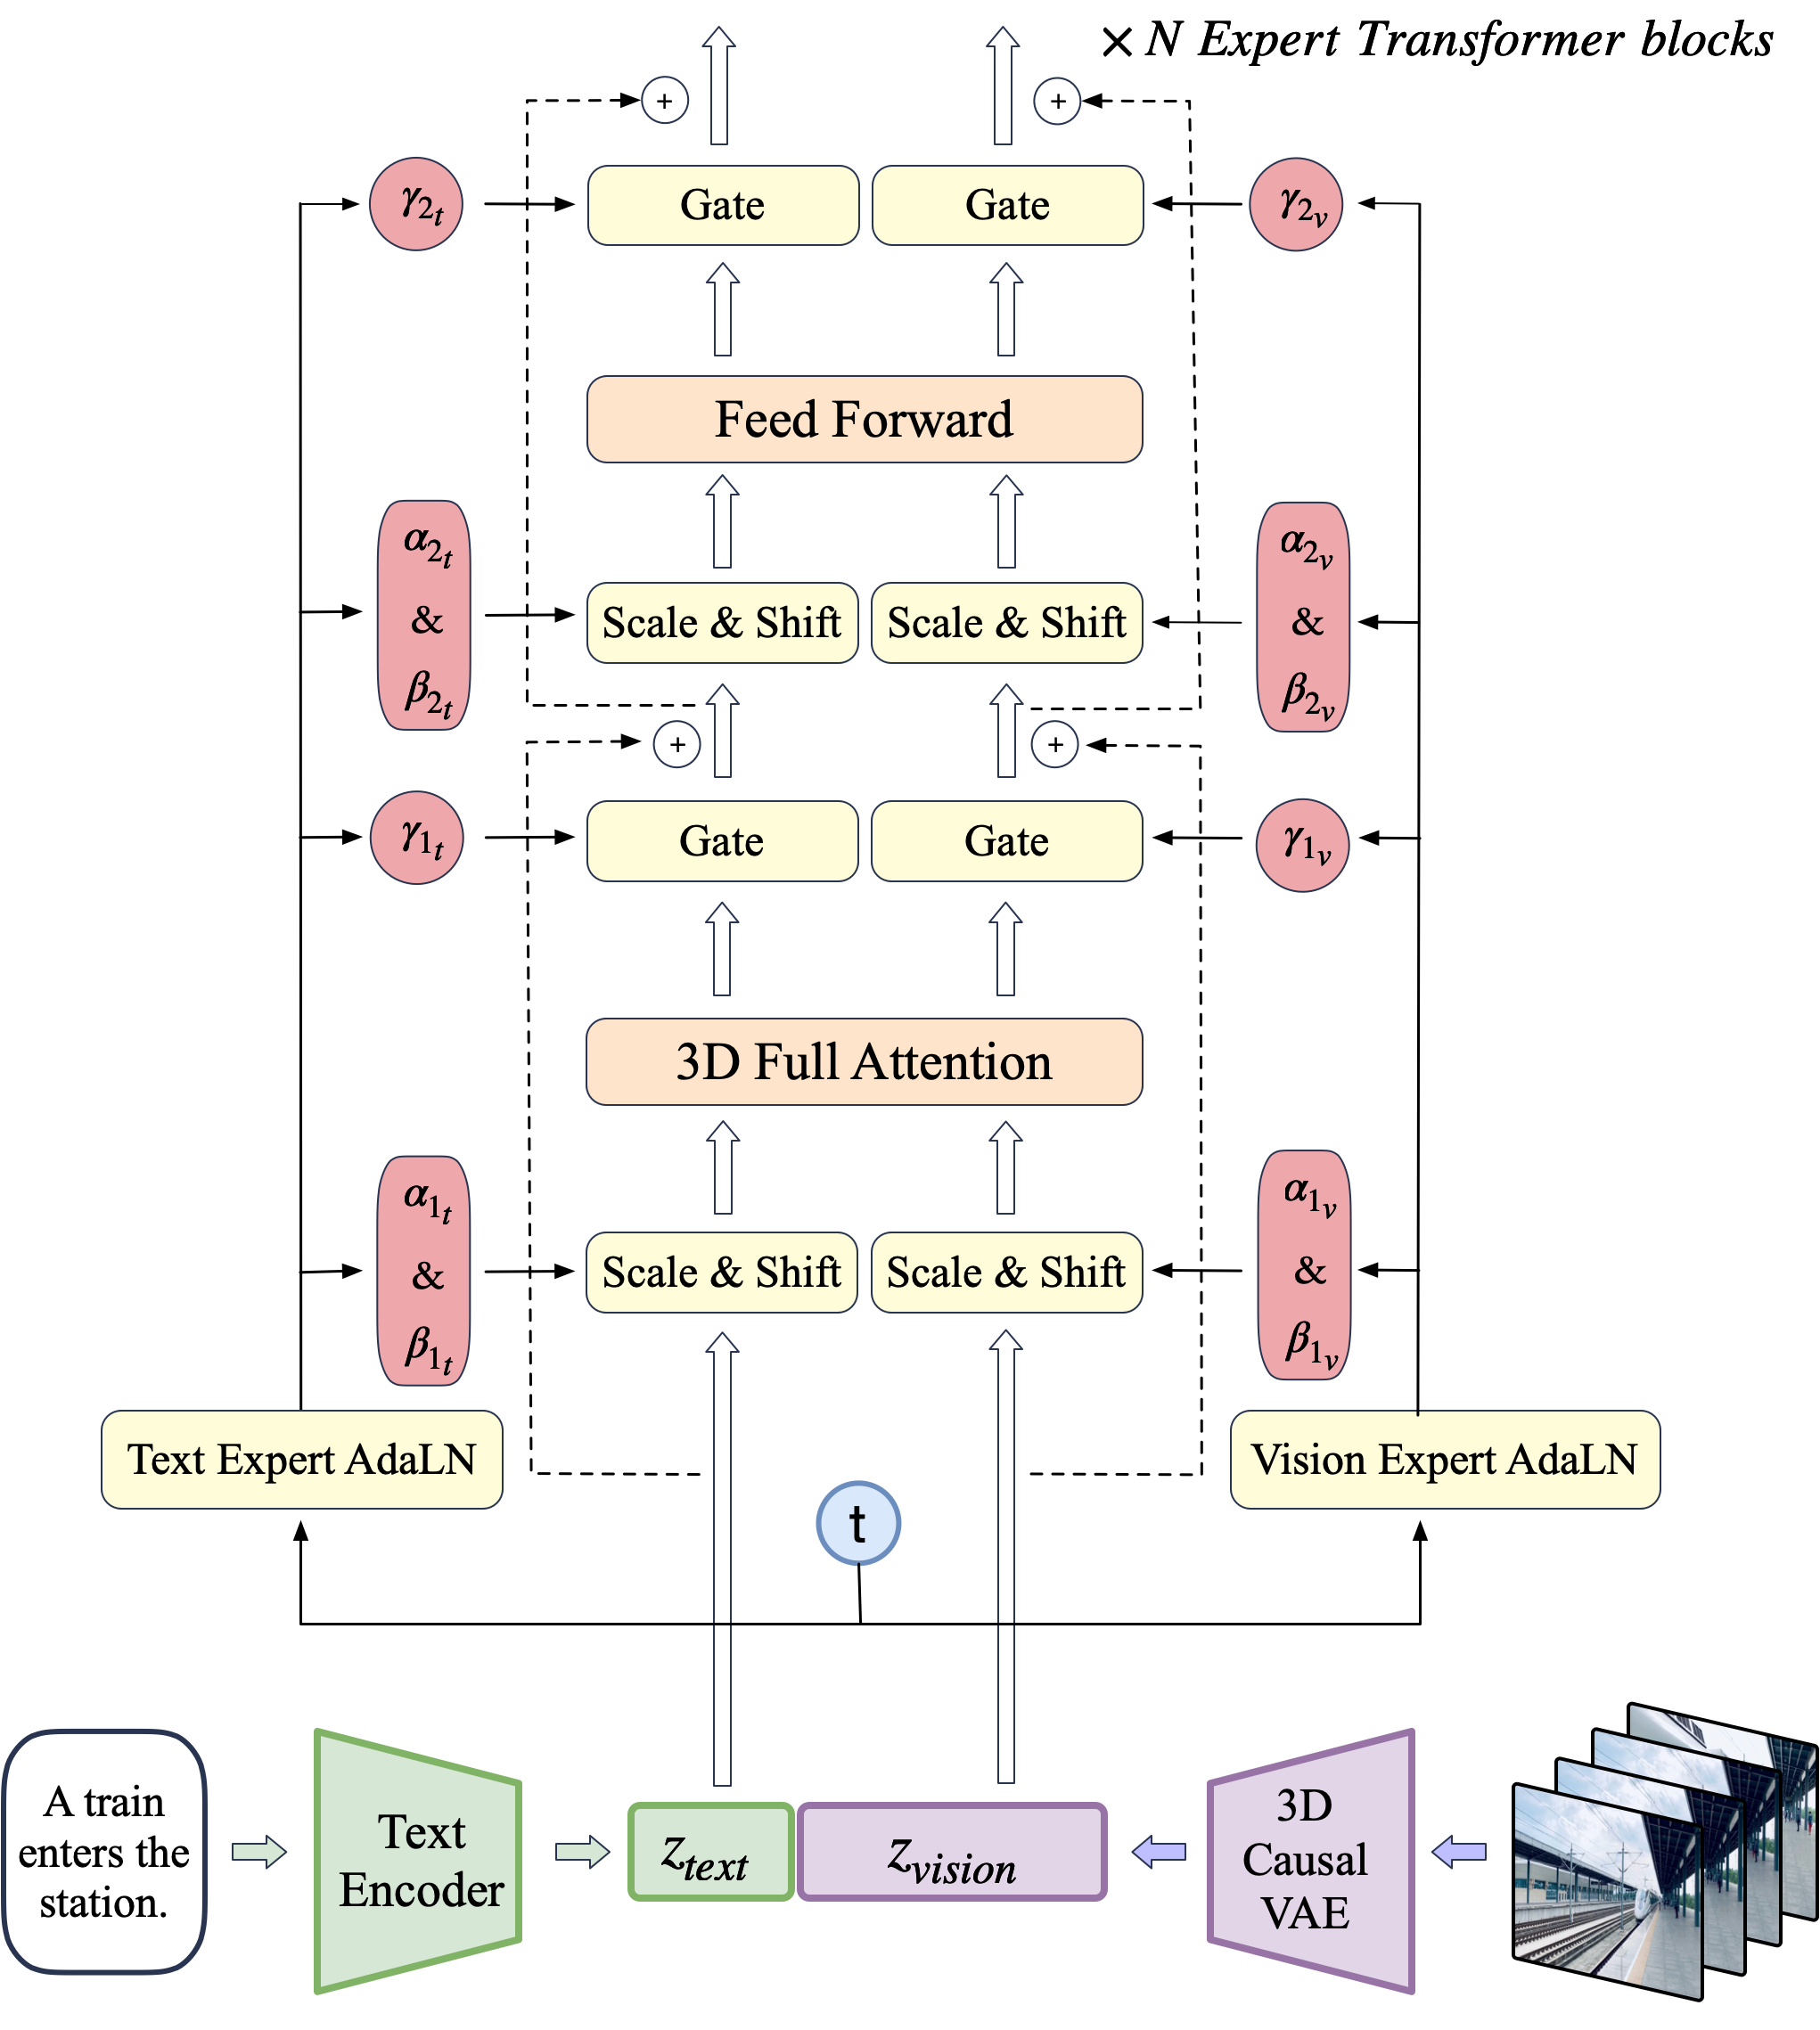
\includegraphics[width=0.7\linewidth]{images/transformer.png}
\end{center}
\caption{\textbf{The overall architecture of \model.} }
\label{fig:model}
\end{figure}



\subsection{3D Causal VAE} 



Videos encompass not only spatial information but also substantial temporal information, usually resulting in orders of magnitude more data volumes than images.  
To tackle the computational challenge of modeling video data, we propose to implement a video compression module based on 3D Variational Autoencoders (3D VAEs)~\cite{yu2023language}.
The idea is to incorporate three-dimentional convolutions to compress videos both spatially and temporally. 
This can help achieve a higher compression ratio with largely improved quality and continuity of video reconstruction when compared to previous image VAEs~\cite{rombach2022high, esser2021taming}. 
\begin{figure}[h]
\begin{center}
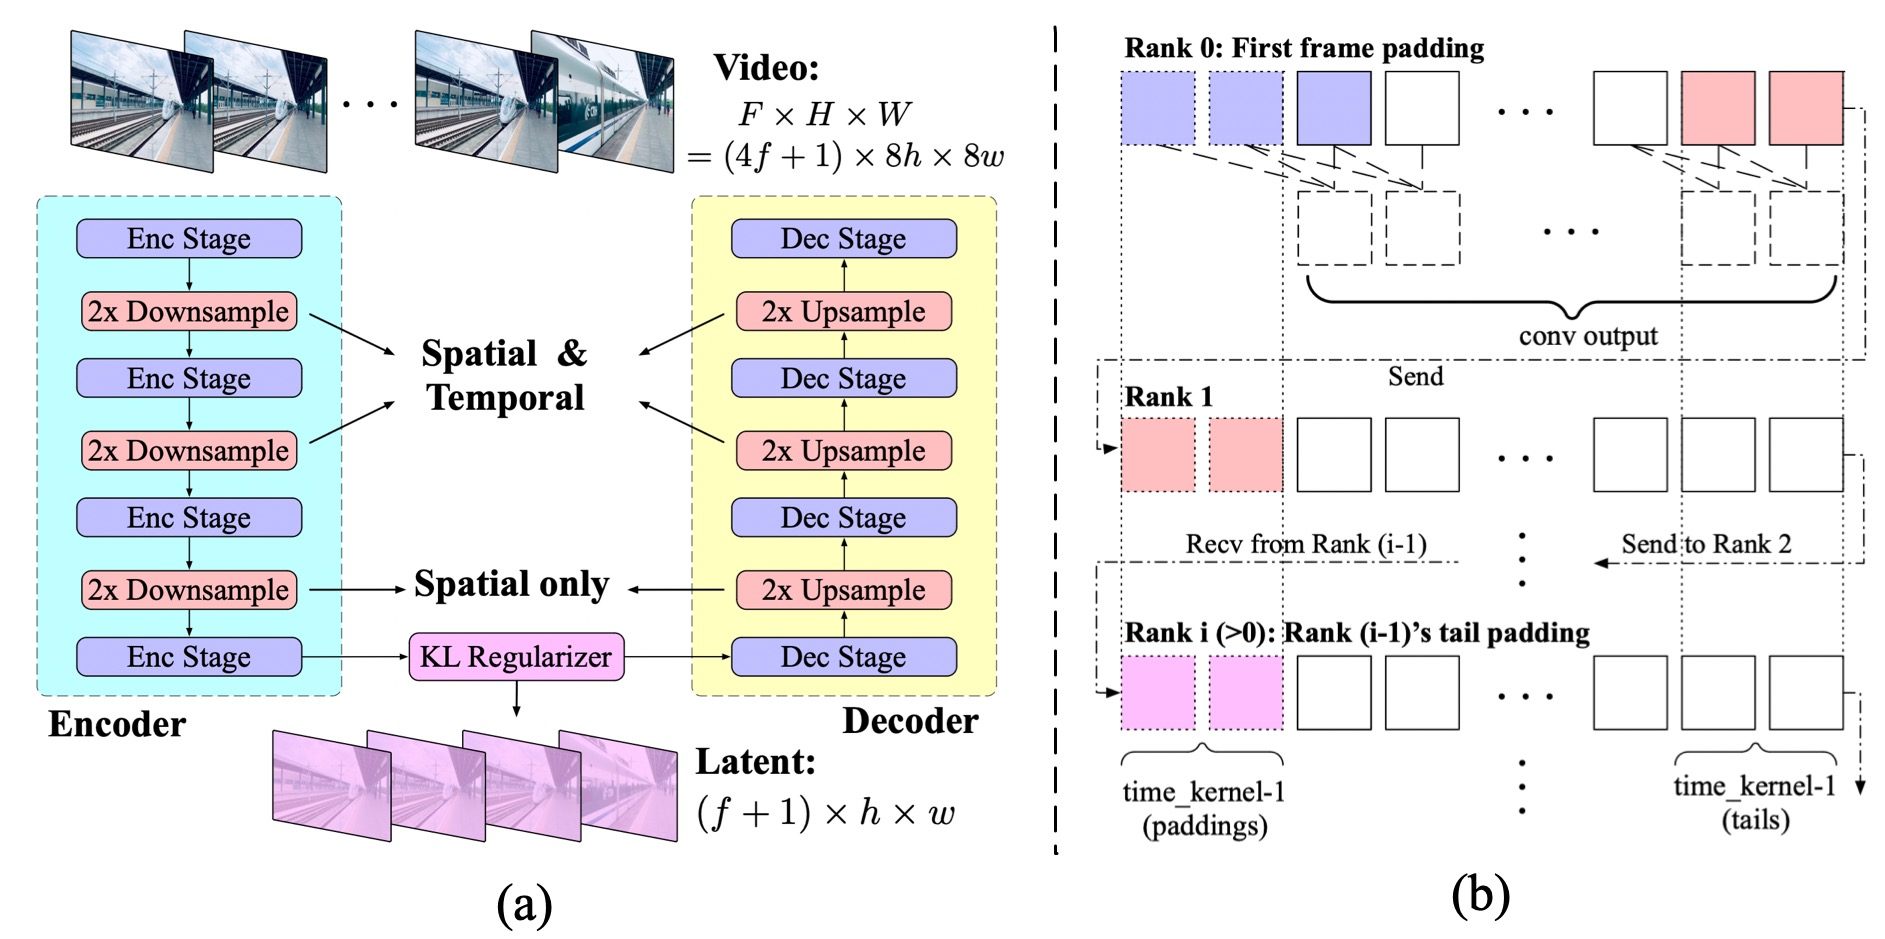
\includegraphics[width=\linewidth]{images/3dvae_combined.jpg}
\end{center}
\caption{(a) The structure of the 3D VAE in \model. It comprises an encoder, a decoder and a latent space regularizer, achieving a 4$\times$8$\times$8 compression from pixels to the latents. (b) The context parallel implementation on the temporally causal convolution.}
\label{fig:3dvae_combined}
\end{figure}

Figure~\ref{fig:3dvae_combined} (a) shows the structure of the proposed 3D VAE. 
It comprises an encoder, a decoder and a latent space regularizer. 
The Gaussian latent space is constrained by a Kullback-Leibler (KL) regularizer.
The encoder and decoder consist of four symmetrically arranged stages, respectively performing 2$\times$ downsampling and upsampling by the interleaving of ResNet block stacked stages. 
The first two rounds of downsampling and the last two upsampling involve both the spatial and temporal dimensions, while the last round only applies spatial sampling. 
This enables the 3D VAE to achieve a 4$\times$ compression in the temporal dimension and an 8$\times$8 compression in the spatial dimension. 
In total, this achieves a 4$\times$8$\times$8 compression from pixels to the latents. 

We adopt the temporally causal convolution~\cite{yu2023language}, which places all the paddings at the beginning of the convolution space, as shown in Figure~\ref{fig:3dvae_combined} (b). 
This ensures the future information not to influence the present or past predictions. 
Given that processing videos with a large number of frames introduces excessive GPU memory usage, we apply context parallel at the temporal dimension for 3D convolution to distribute computation among multiple devices. 
As illustrated by Figure~\ref{fig:3dvae_combined} (b), due to the causal nature of the convolution, each rank simply sends a segment of length $k-1$ to the next rank, where $k$ indicates the temporal kernel size. 
This results in relatively low communication overhead.

During actual implementation, we first train a 3D VAE on lower resolutions and fewer frames to save computation. 
We observe that the encoding of larger resolution generalizes naturally, while extending the number of frames to be encoded does not work as seamlessly. 
Therefore, we conduct a two-stage training process by first training on short videos and finetuning by context parallel on long videos. 
Both stages of training utilize a weighted combination of the L2 loss, LPIPS~\cite{zhang2018unreasonable} perceptual loss, and GAN loss from a 3D discriminator.
 
\subsection{Expert Transformer}\label{sec:expert-transformer}

We introduce the design choices in Transformer for \model, including the patching, positional embedding, and attention strategies for handling the text-video data effectively and efficiently. 

\paragraph{Patchify.}
The 3D causal VAE encodes a video latent vector of shape $T \times H \times W \times C$, where $T$ represents the number of frames, $H$ and $W$ represent the height and width of each frame, $C$ represents the channel number, respectively.
The video latents are then patchified  along the spatial dimensions, generating sequence $z_{\text{vision}}$ of length $T\cdot \frac{H}{p} \cdot \frac{W}{p}$. 
Note that, we do not patchify along the temporal dimension in order to enable joint training of images and videos.

\paragraph{3D-RoPE.}
Rotary Position Embedding (RoPE)~\cite{su2024roformer} is a relative positional encoding that has been demonstrated to capture inter-token relationships effectively in LLMs, particularly excelling in modeling long sequences. 
To adapt to video data, we extend the original RoPE to 3D-RoPE. 
Each latent in the video tensor can be represented by a 3D coordinate $(x, y, t)$.
We independently apply 1D-RoPE to each dimension of the coordinates, each occupying $3/8$, $3/8$, and $2/8$ of the hidden states' channel. 
The resulting encoding is then concatenated along the channel dimension to obtain the final 3D-RoPE encoding. 

We empirically examine the use of RoPE. 
Figure~\ref{fig:subfigures} (a)shows the comparison between 3D RoPE and sinusoidal absolute position encoding. 
We can observe that the loss curve using 3D RoPE converges significantly faster than that with sinusoidal encoding. 
We further compare the use of 3D RoPE alone against the combination of 3D RoPE and learnable absolute position embedding. 
Figure~\ref{fig:subfigures} (b) indicates that the loss curves of both methods converge almost identically. 
Therefore, we choose to use 3D RoPE alone for simplicity. 


\begin{figure}[h]
    \centering
    \begin{subfigure}[b]{0.46\textwidth}
        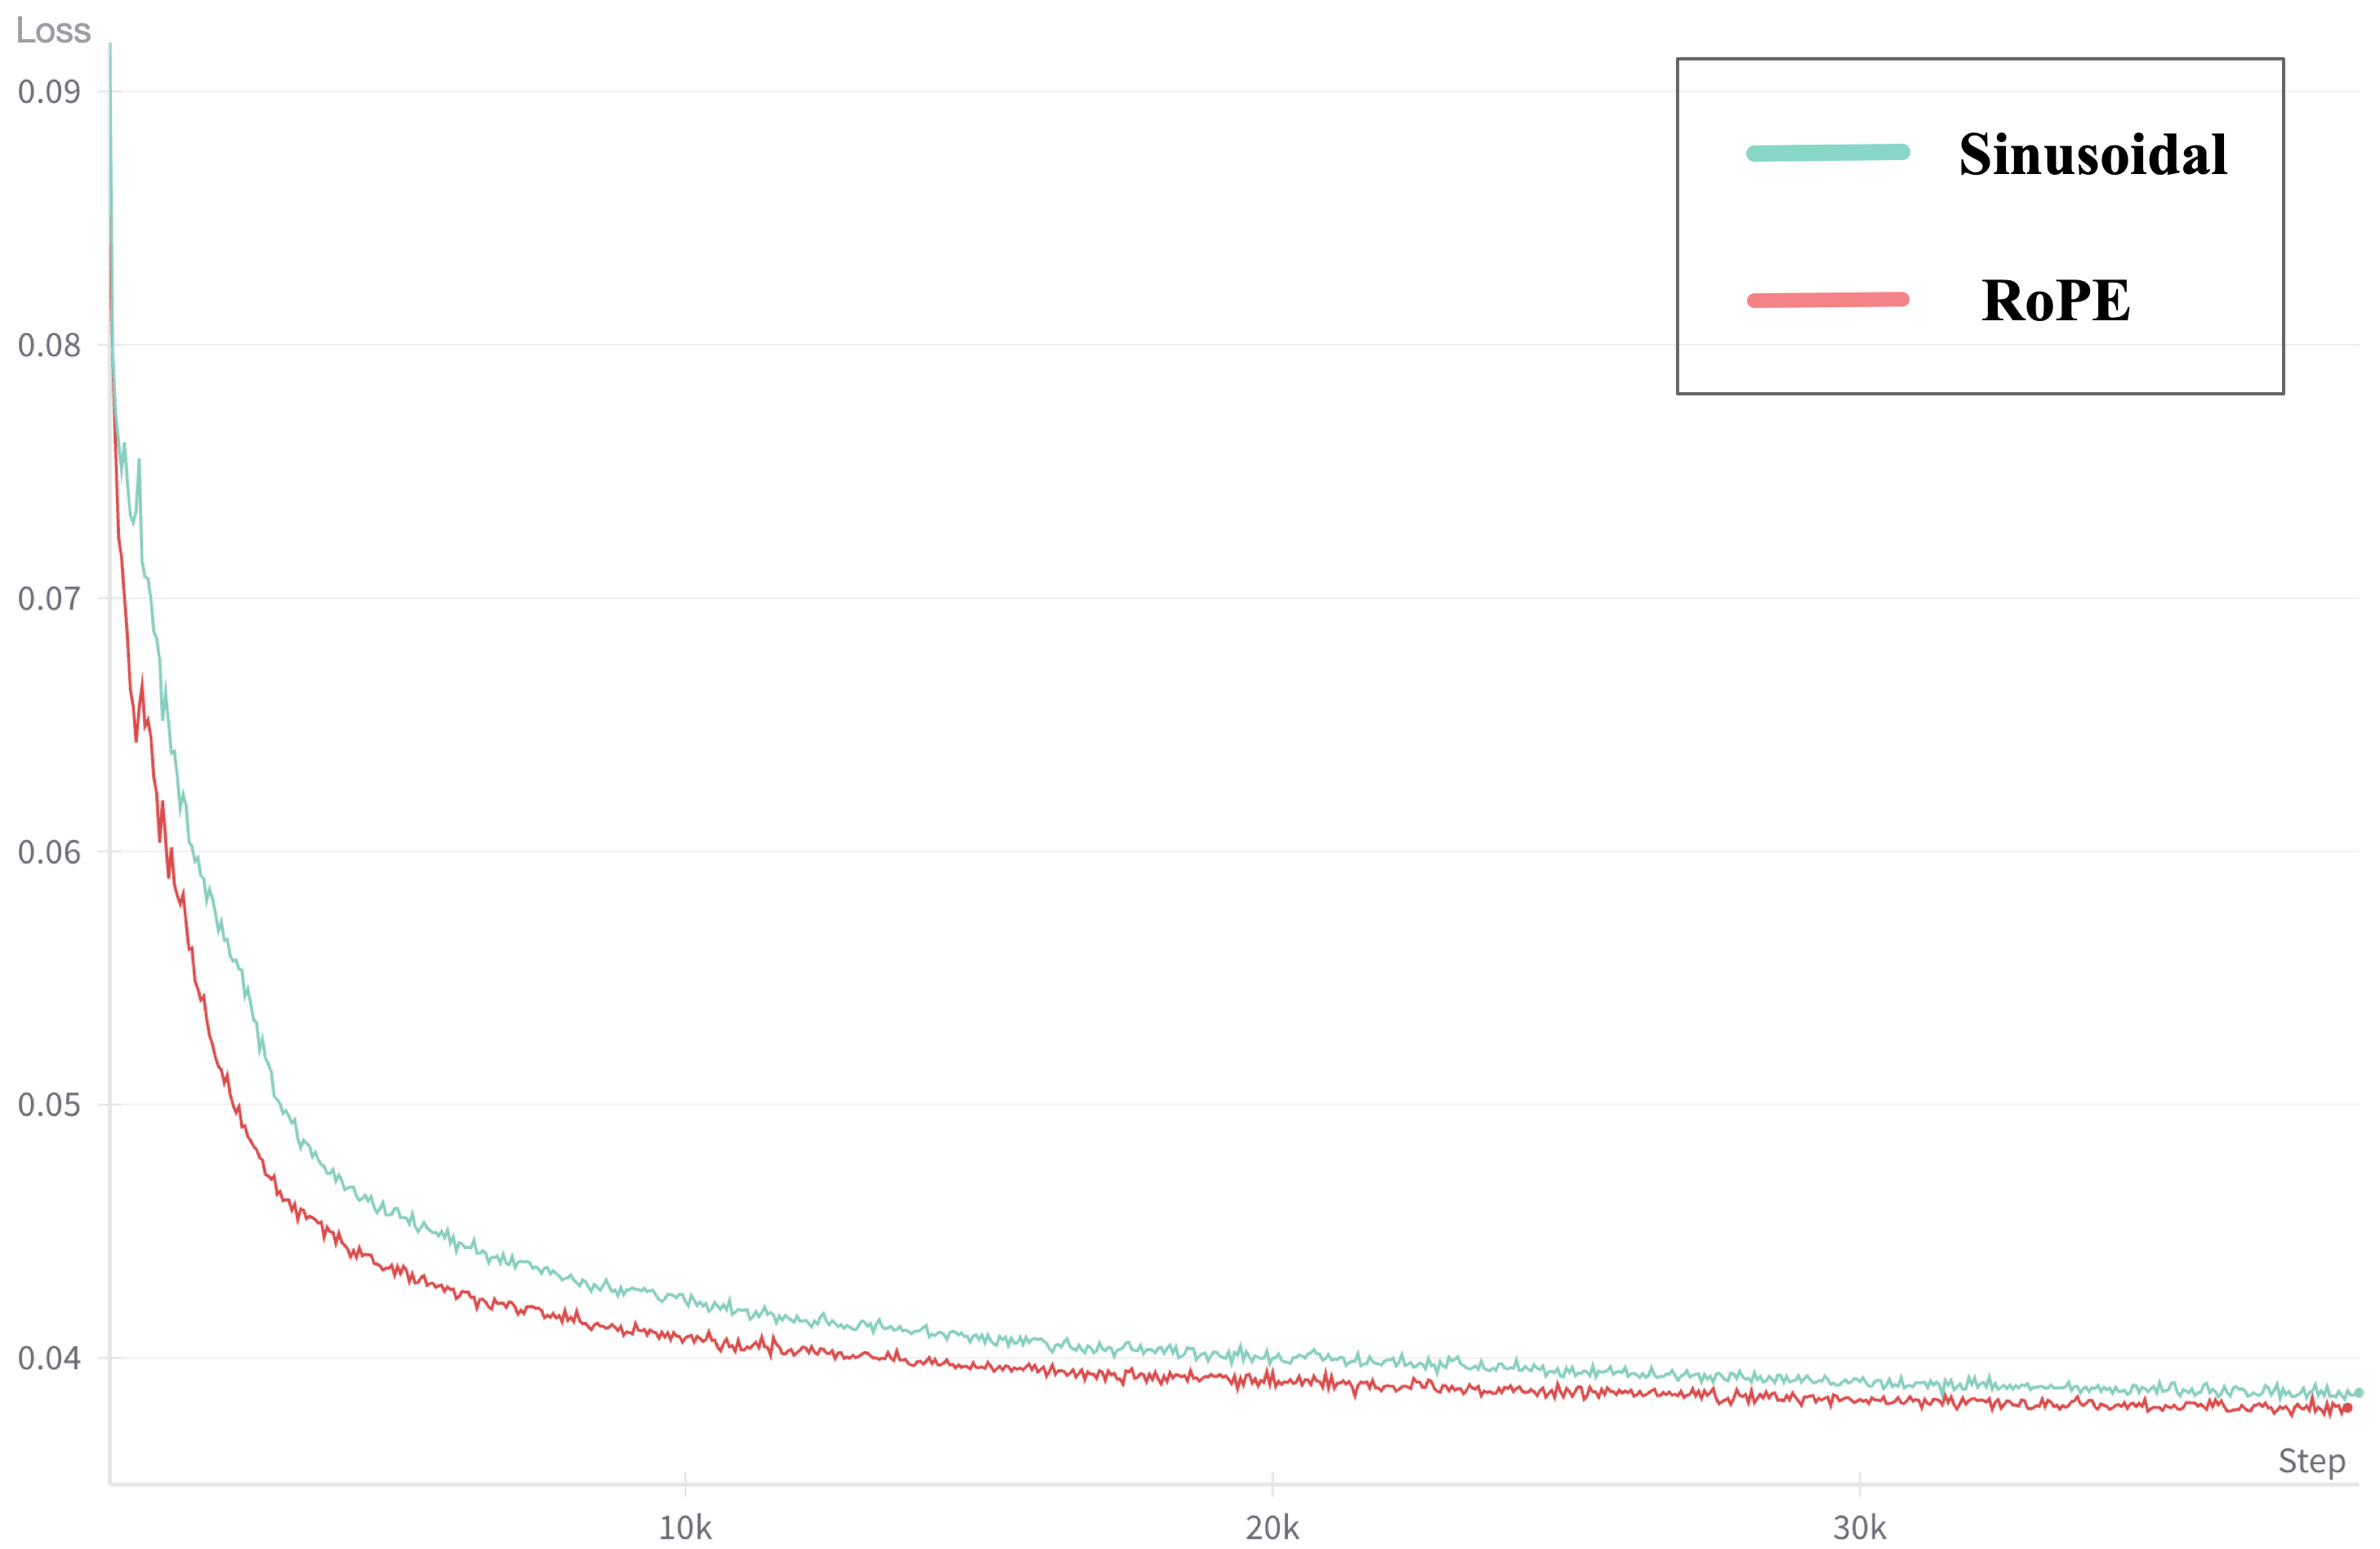
\includegraphics[width=\textwidth]{images/ab_sr.png}
        \caption{RoPE vs. Sinusoidal}
        \label{fig:rope-sin}
    \end{subfigure}
    \begin{subfigure}[b]{0.48\textwidth}
        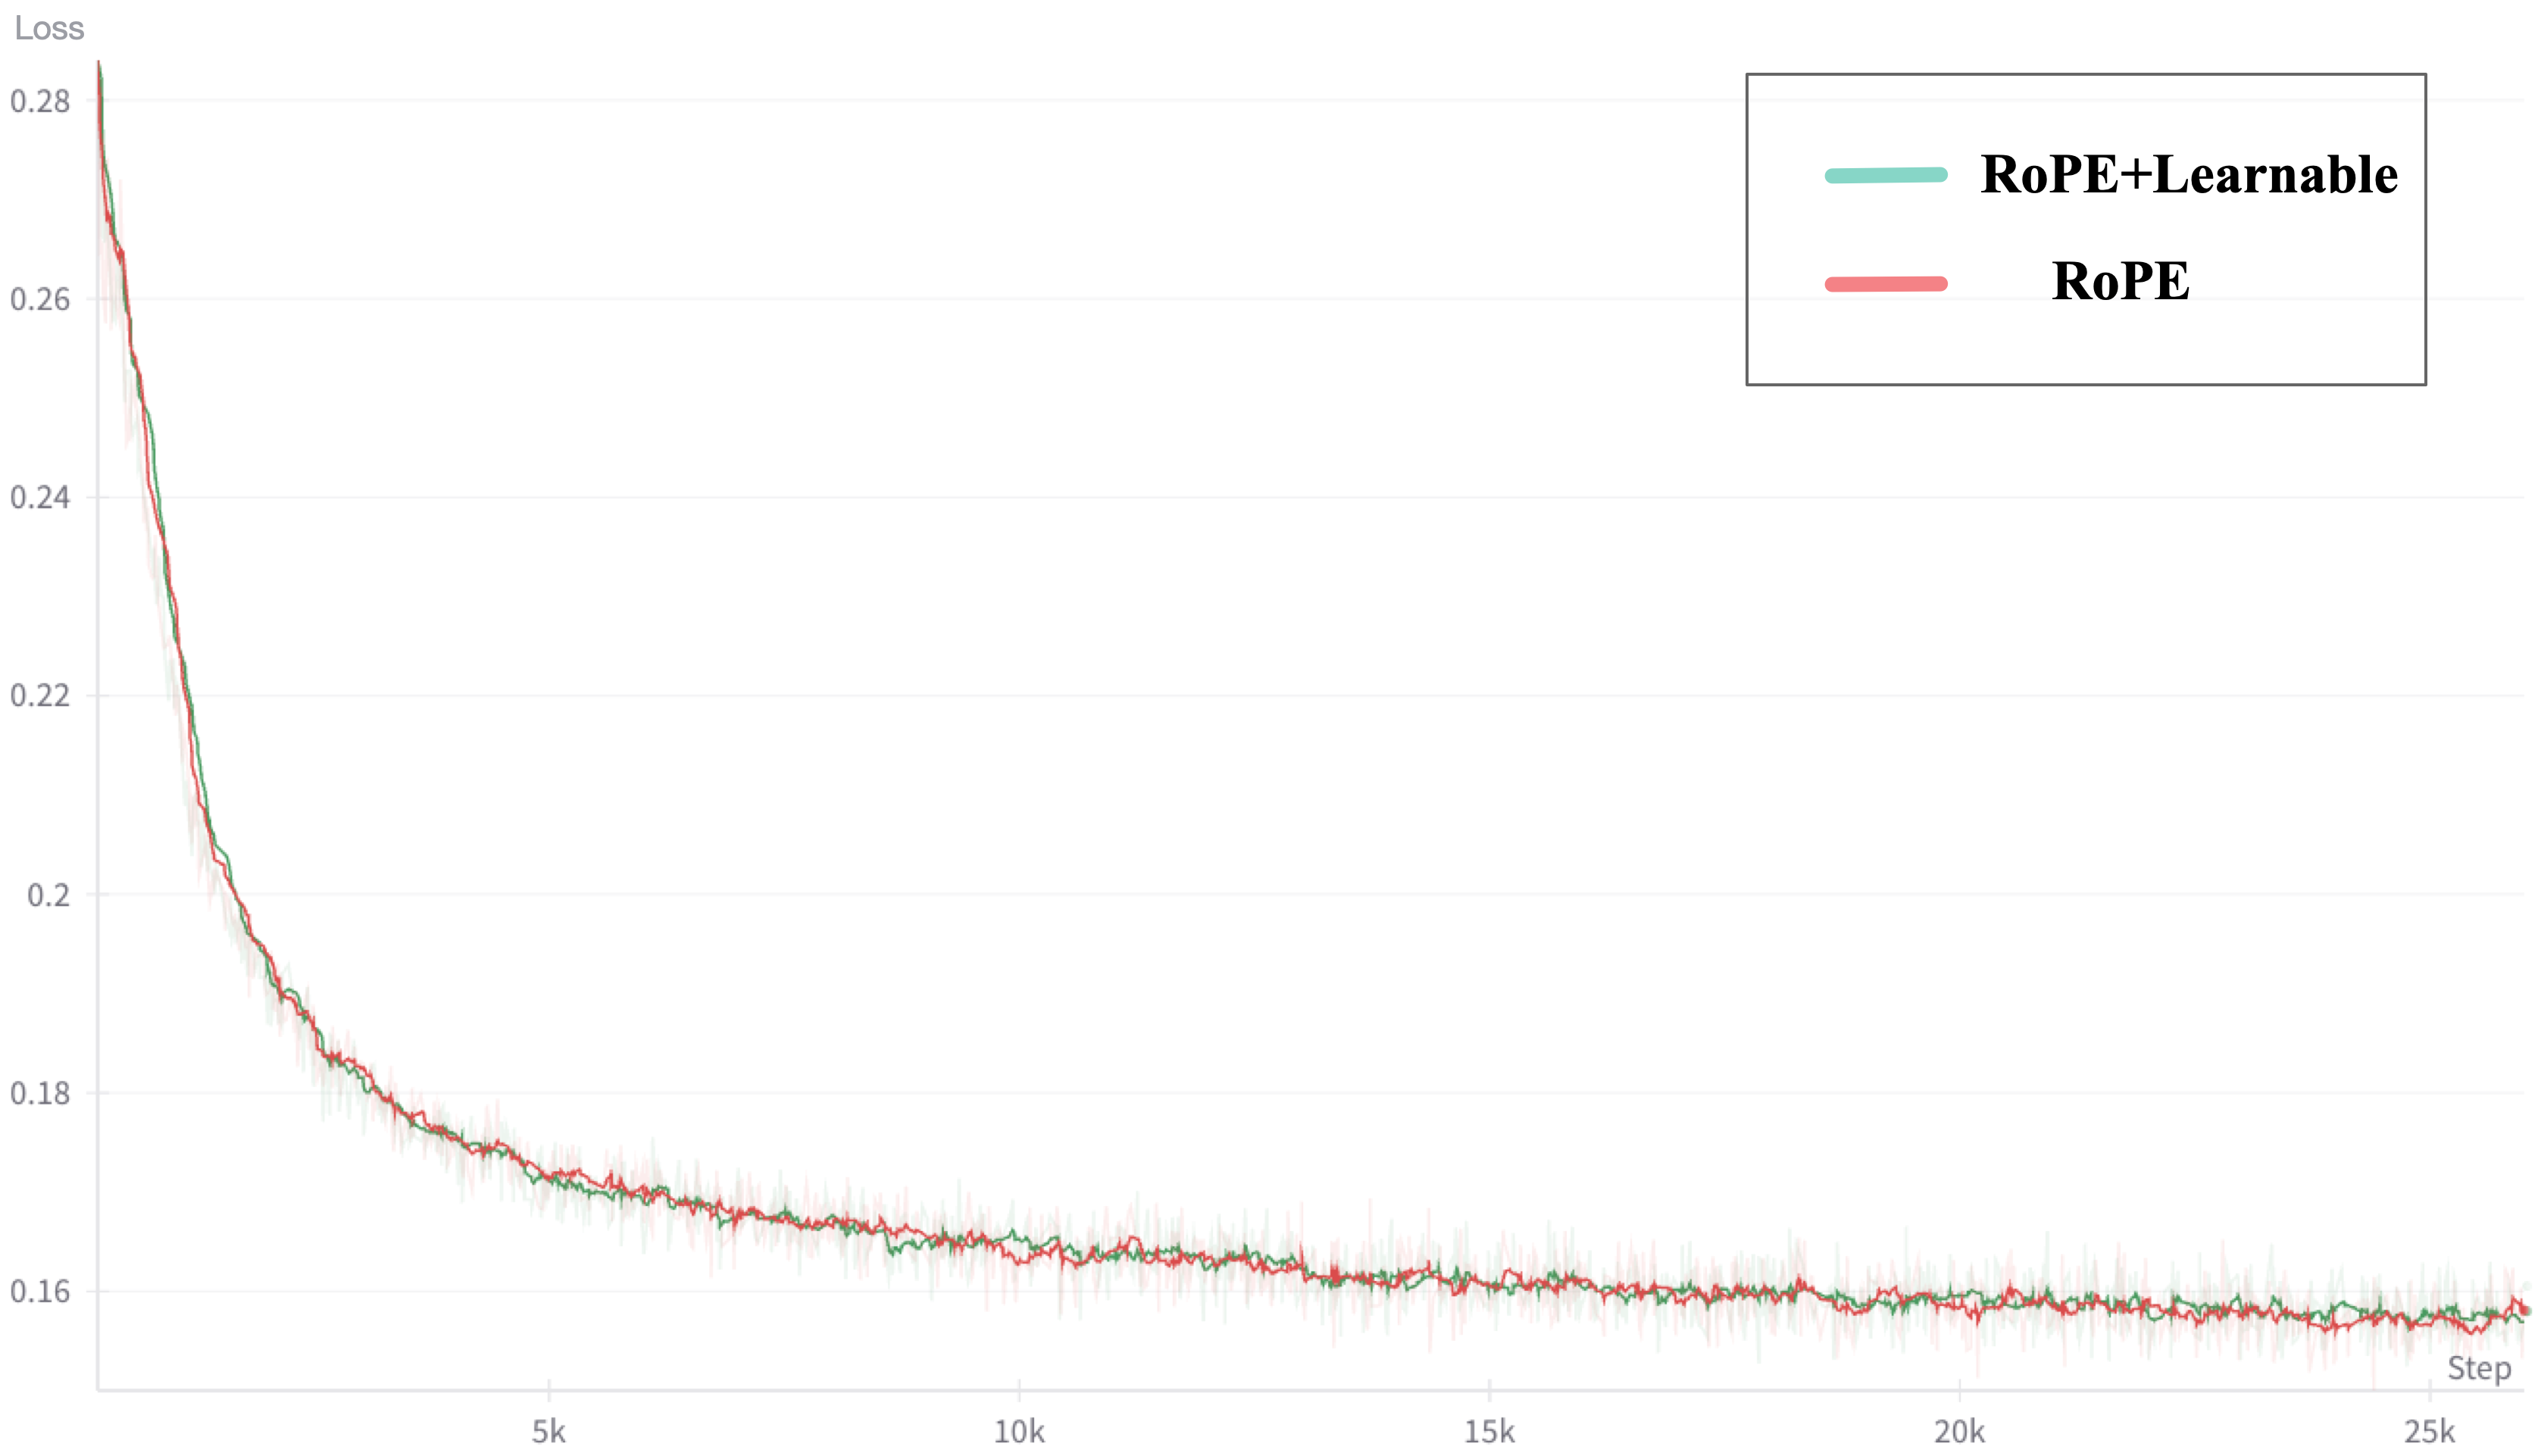
\includegraphics[width=\textwidth]{images/ab_rl.png}
        \caption{RoPE vs. RoPE + Learnable}
        \label{fig:rope-learnable}
    \end{subfigure}
    \begin{subfigure}[b]{0.46\textwidth}
        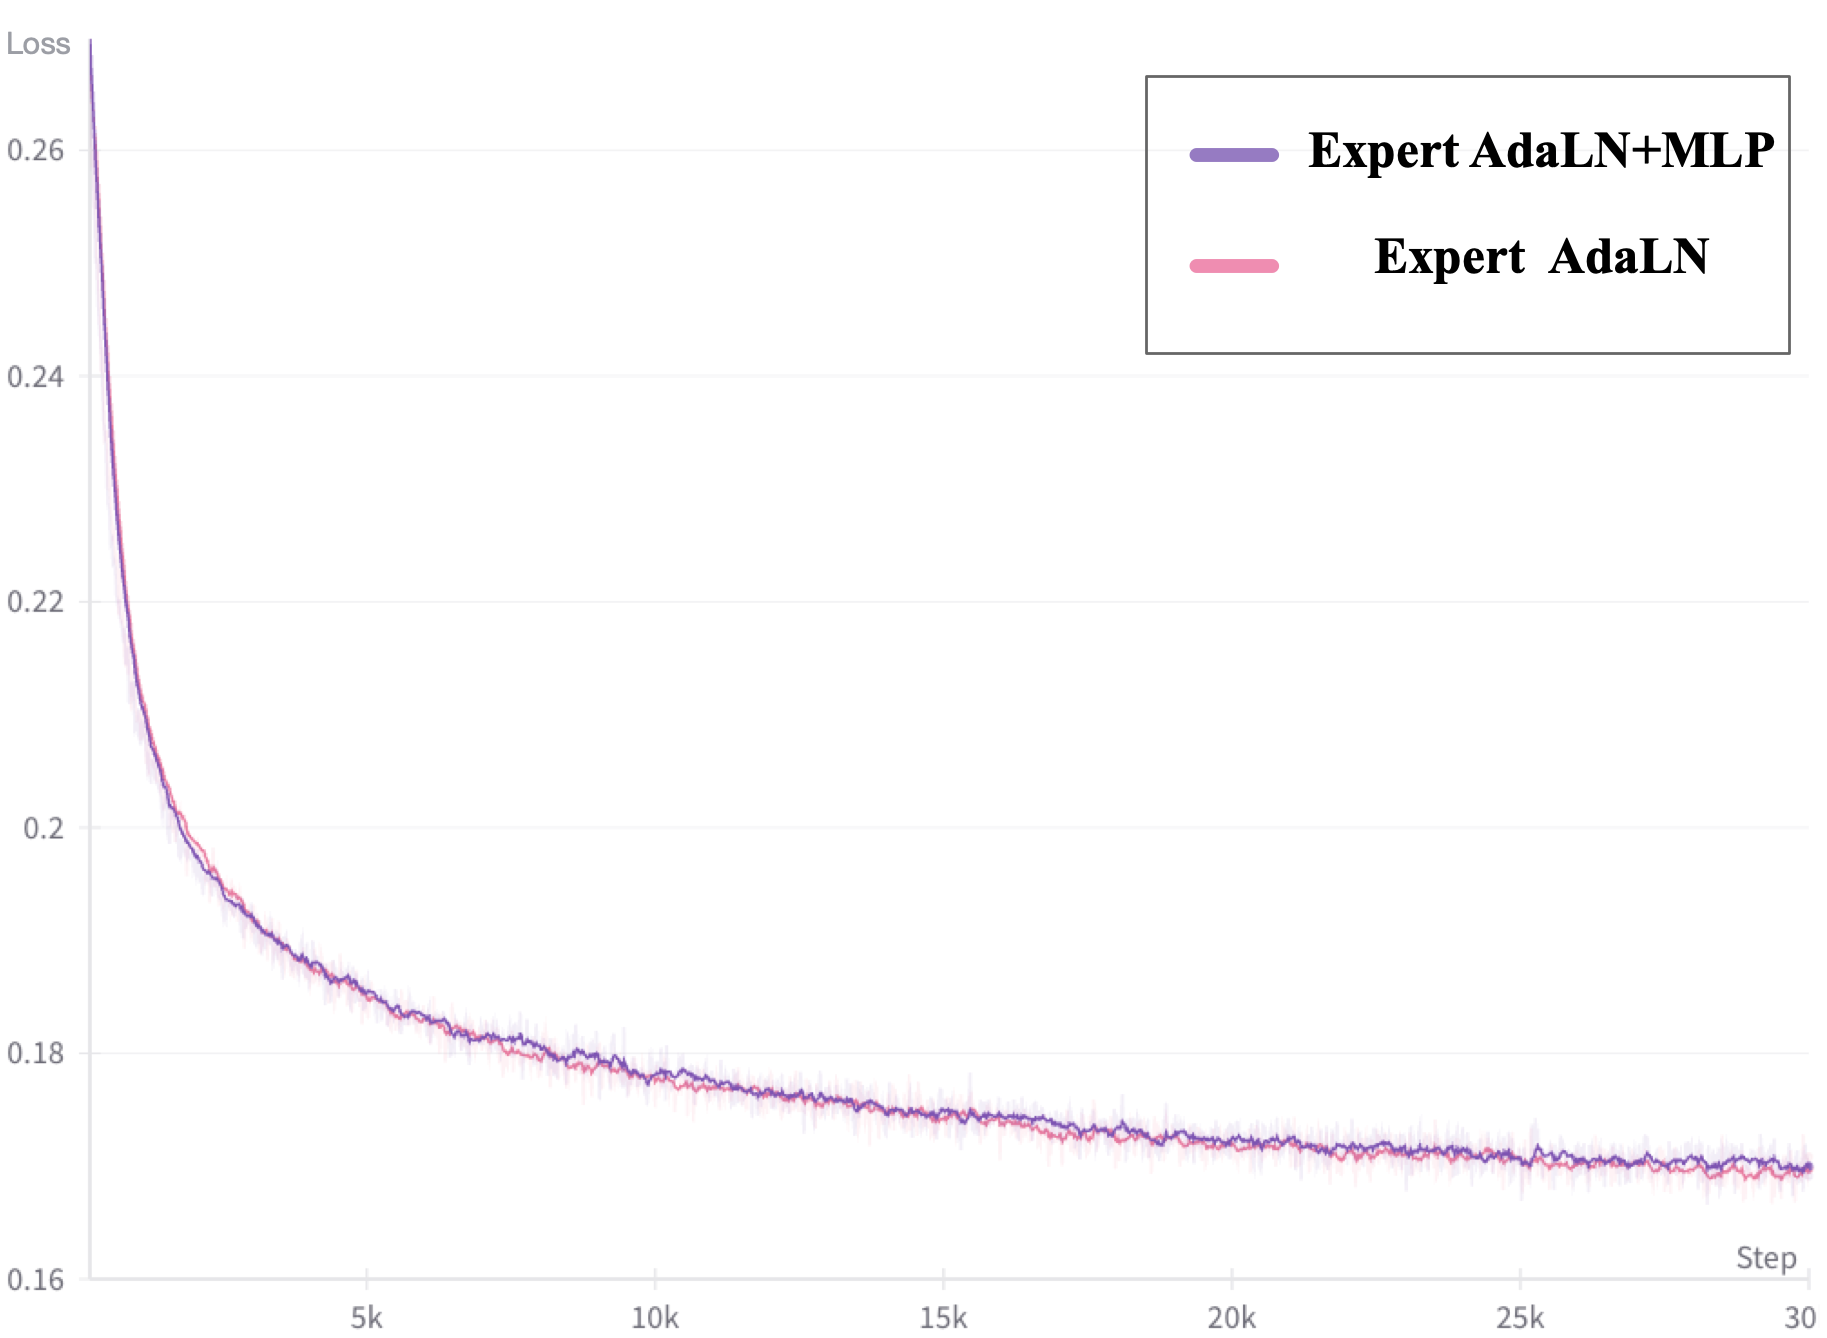
\includegraphics[width=\textwidth]{images/ab_ex.png}
        \caption{Expert Ada. LN vs. Expert Ada. LN + MLP}
        \label{fig:expert}
    \end{subfigure}
    \begin{subfigure}[b]{0.48\textwidth}
        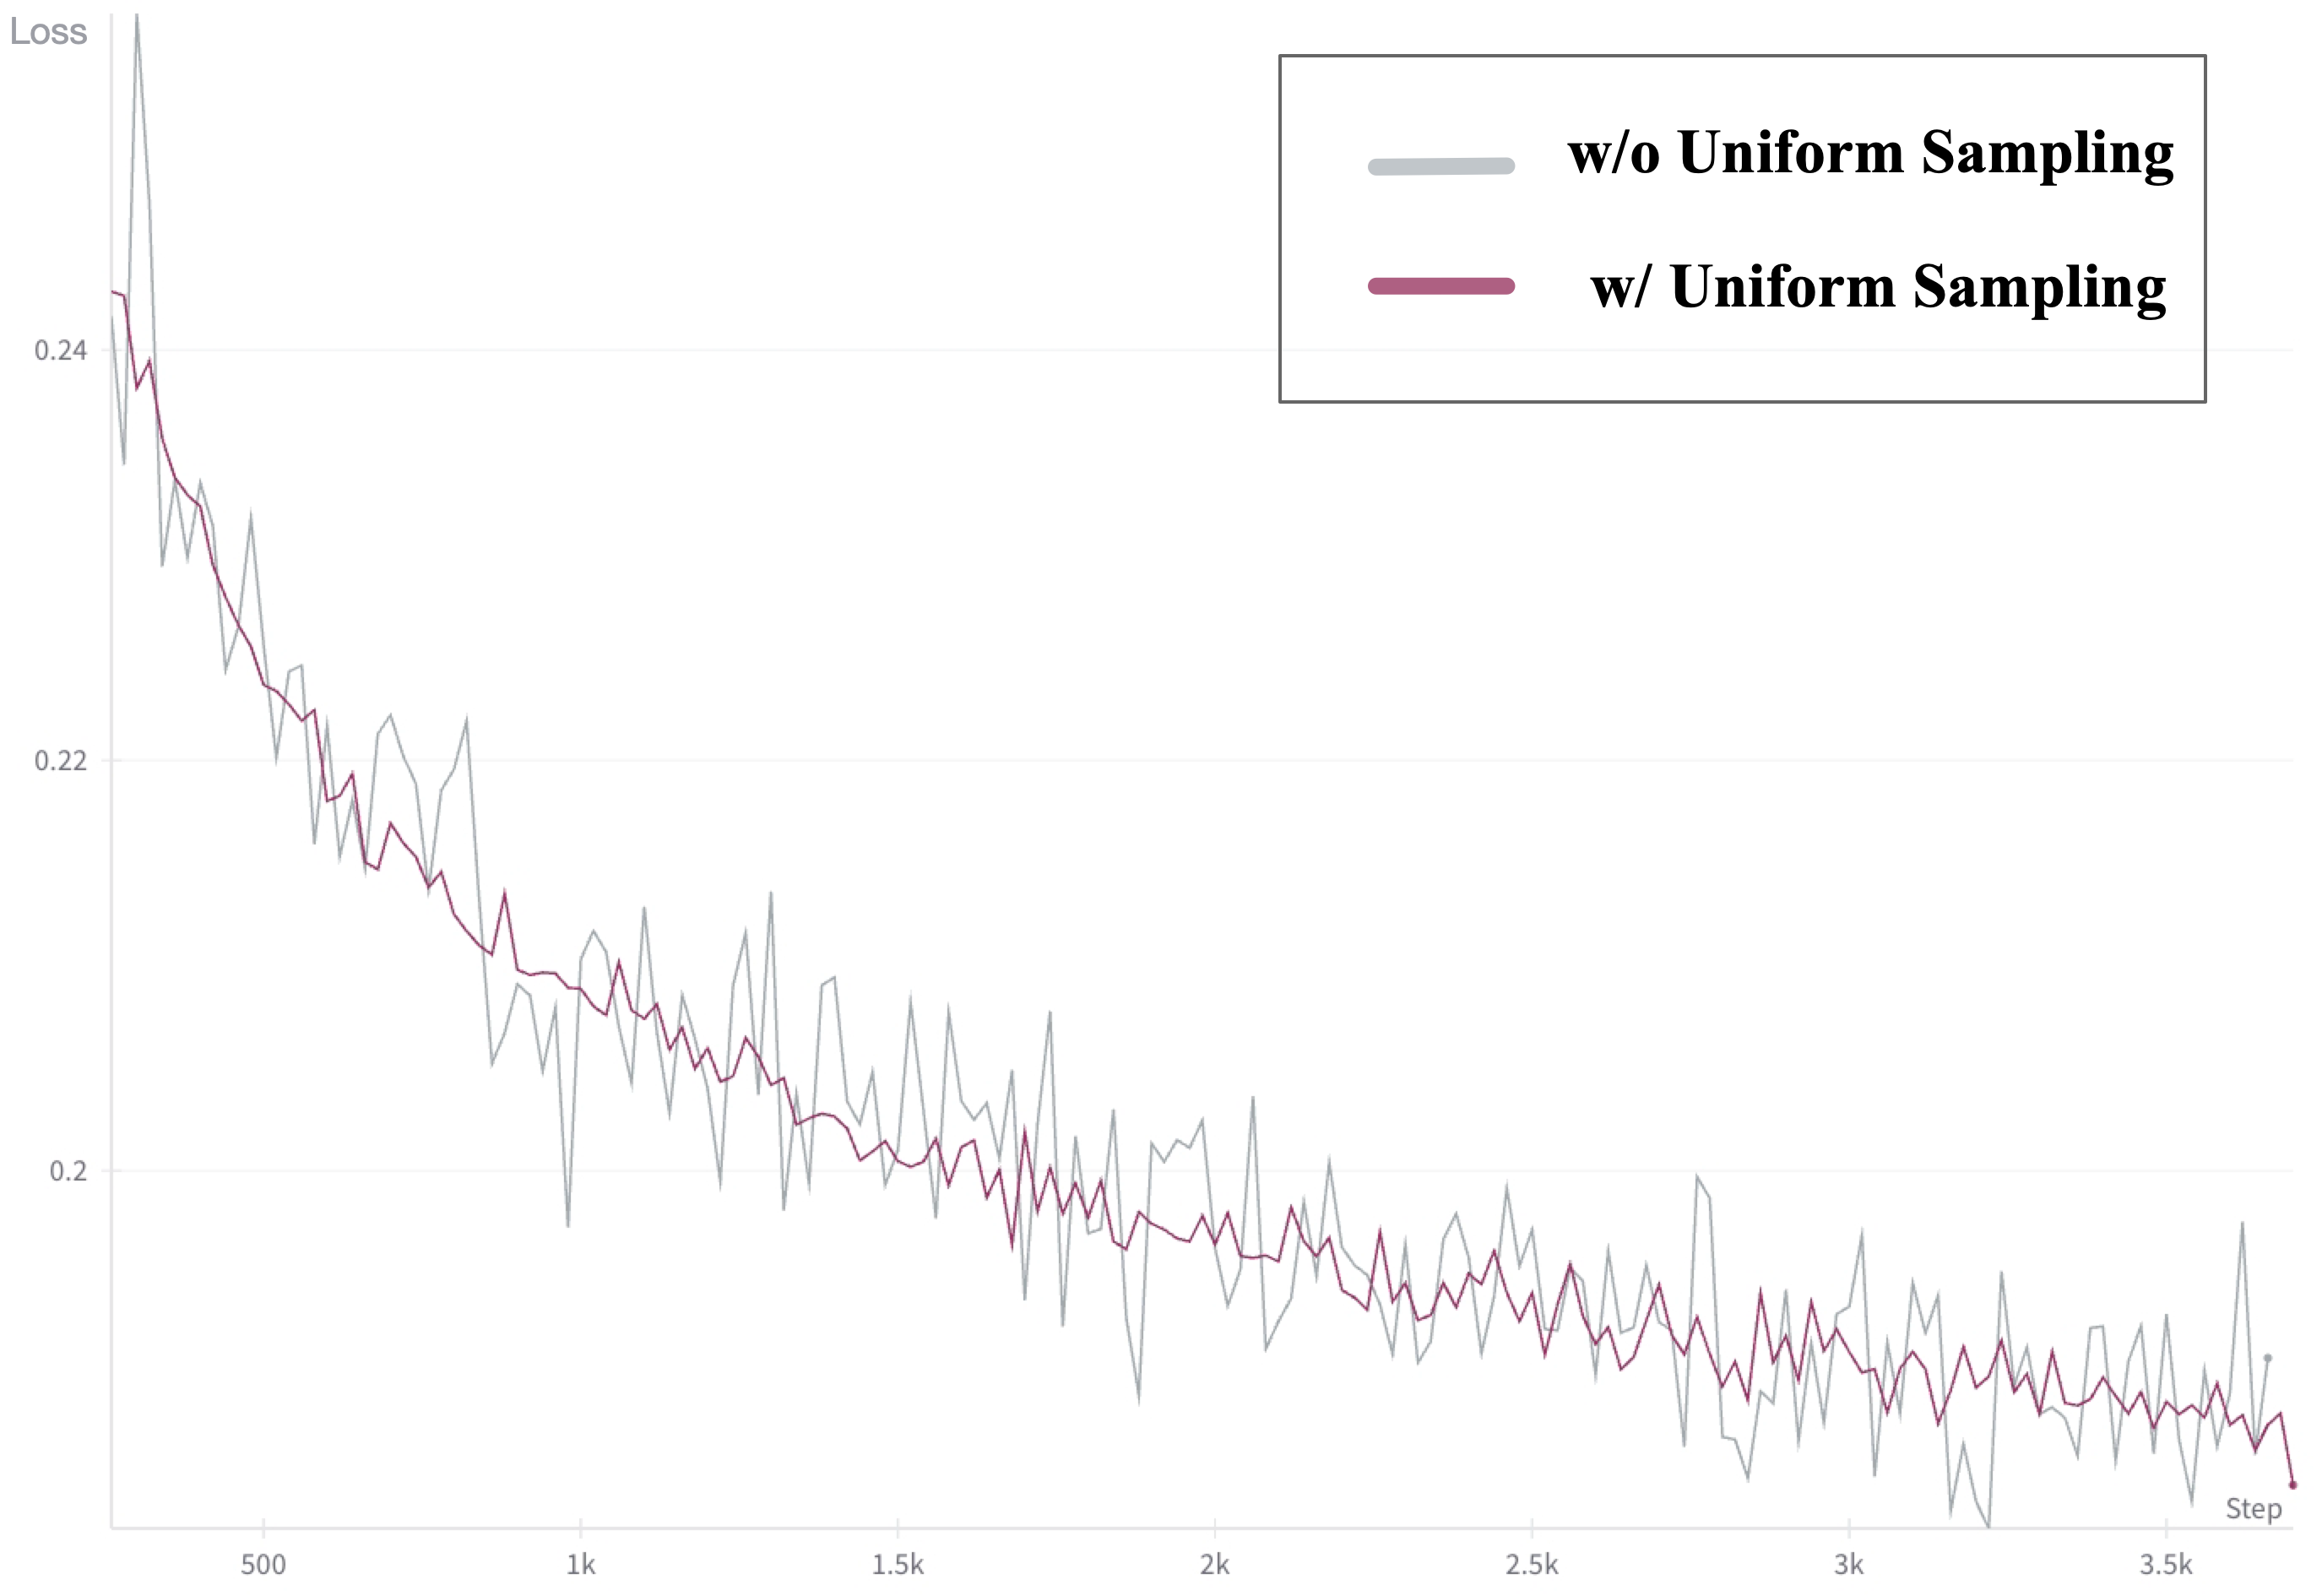
\includegraphics[width=\textwidth]{images/ab_us.png}
        \caption{Uniform Sampling vs. No Uniform Sampling}
        \label{fig:uniform-sampling}
    \end{subfigure}

    \caption{Training loss curve of different ablations.}
    \label{fig:subfigures}
\end{figure}



\paragraph{Expert Transformer Block.}
We concatenate the embeddings of both text and video at the input stage to better align visual and semantic information. 
However, the feature spaces of these two modalities differ significantly, and their embeddings may even have different numerical scales. 
To better process them within the same sequence, we employ the Expert Adaptive Layernorm to handle each modality independently.
As shown in Figure~\ref{fig:model}, following DiT~\cite{peebles2023scalable}, we use the timestep $t$ of the diffusion process as the input to the modulation module. 
Then, the Vision Expert Adaptive Layernorm (Vison Expert AdaLN) and Text Expert Adaptive Layernorm (Text Expert AdaLN) apply this modulation mechanism to the vision hidden states and text hidden states, respectively. 
This strategy promotes the alignment of feature spaces across two modalities while minimizing additional parameters.

To verify the adoption of Expert Adaptive Layernorm, we experiment with different ways of incorporating experts: expert LayerNorm and MLP, and expert Layernorm only. 
Our experiments find that adding expert MLP does not effectively accelerate the model's convergence (Cf. Figure~\ref{fig:subfigures} (c)). 
To reduce the model parameters, we only choose to use Expert Adaptive Layernorm.

\begin{figure}[h]
\centering
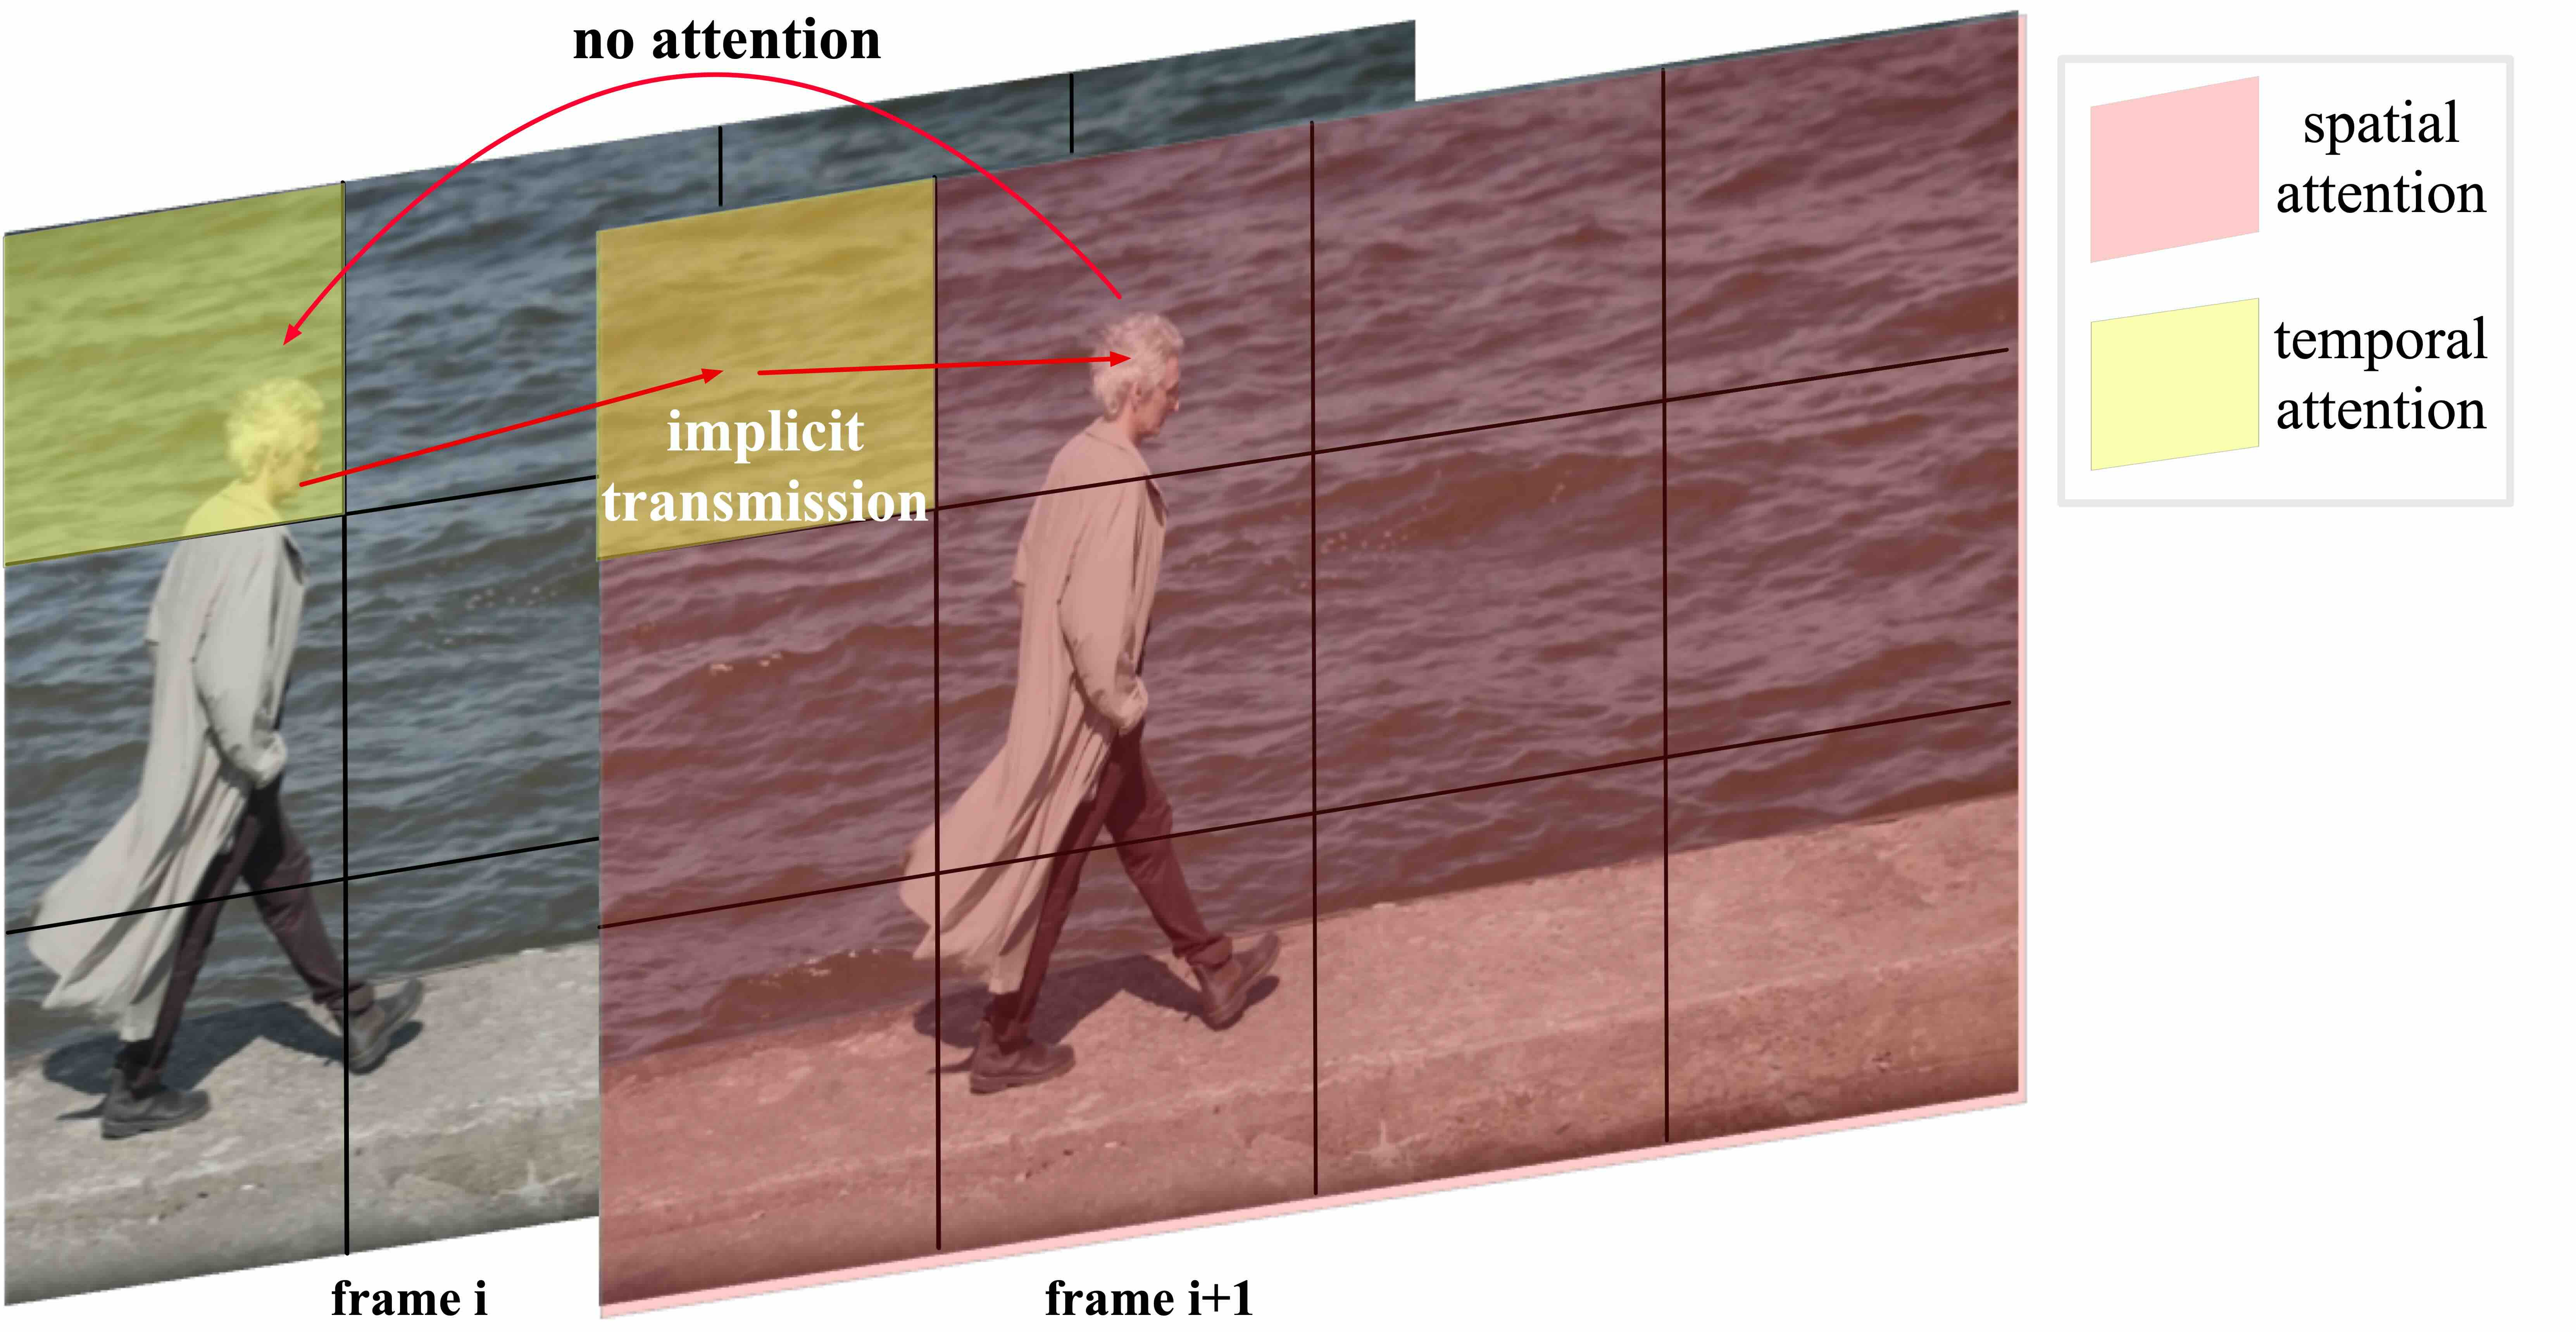
\includegraphics[width=0.7\linewidth]{images/attention.jpg}
\caption{The separated spatial and temporal attention makes it challenging to  handle the large motion between adjacent frames. 
In the figure, the head of the person in frame $i+1$ cannot directly attend to the head in frame $i$. 
Instead, visual information can only be implicitly transmitted through other background patches. 
This can lead to inconsistency issues in the generated videos.}
\label{fig:attention}
\end{figure}


\paragraph{3D Full Attention.}
Previous works \cite{singer2022make, guo2023animatediff} often employ separated spatial and temporal attention to reduce computational complexity and facilitate fine-tuning from text-to-image models. 
However, as illustrated in Figure~\ref{fig:attention}, this separated attention approach requires extensive implicit transmission of visual information, significantly increasing the learning complexity and making it challenging to maintain the consistency of large-movement objects. 
Considering the great success of long-context training in LLMs~\cite{llama3modelcard, bai2024longalign, xiong2023effective}  and the efficiency of FlashAttention~\cite{dao2022flashattention},  we propose a 3D text-video hybrid attention mechanism. 
This mechanism not only achieves better results but can also be easily adapted to various parallel acceleration methods. 


\hide{
\begin{wrapfigure}{r}{0.5\textwidth}
\centering
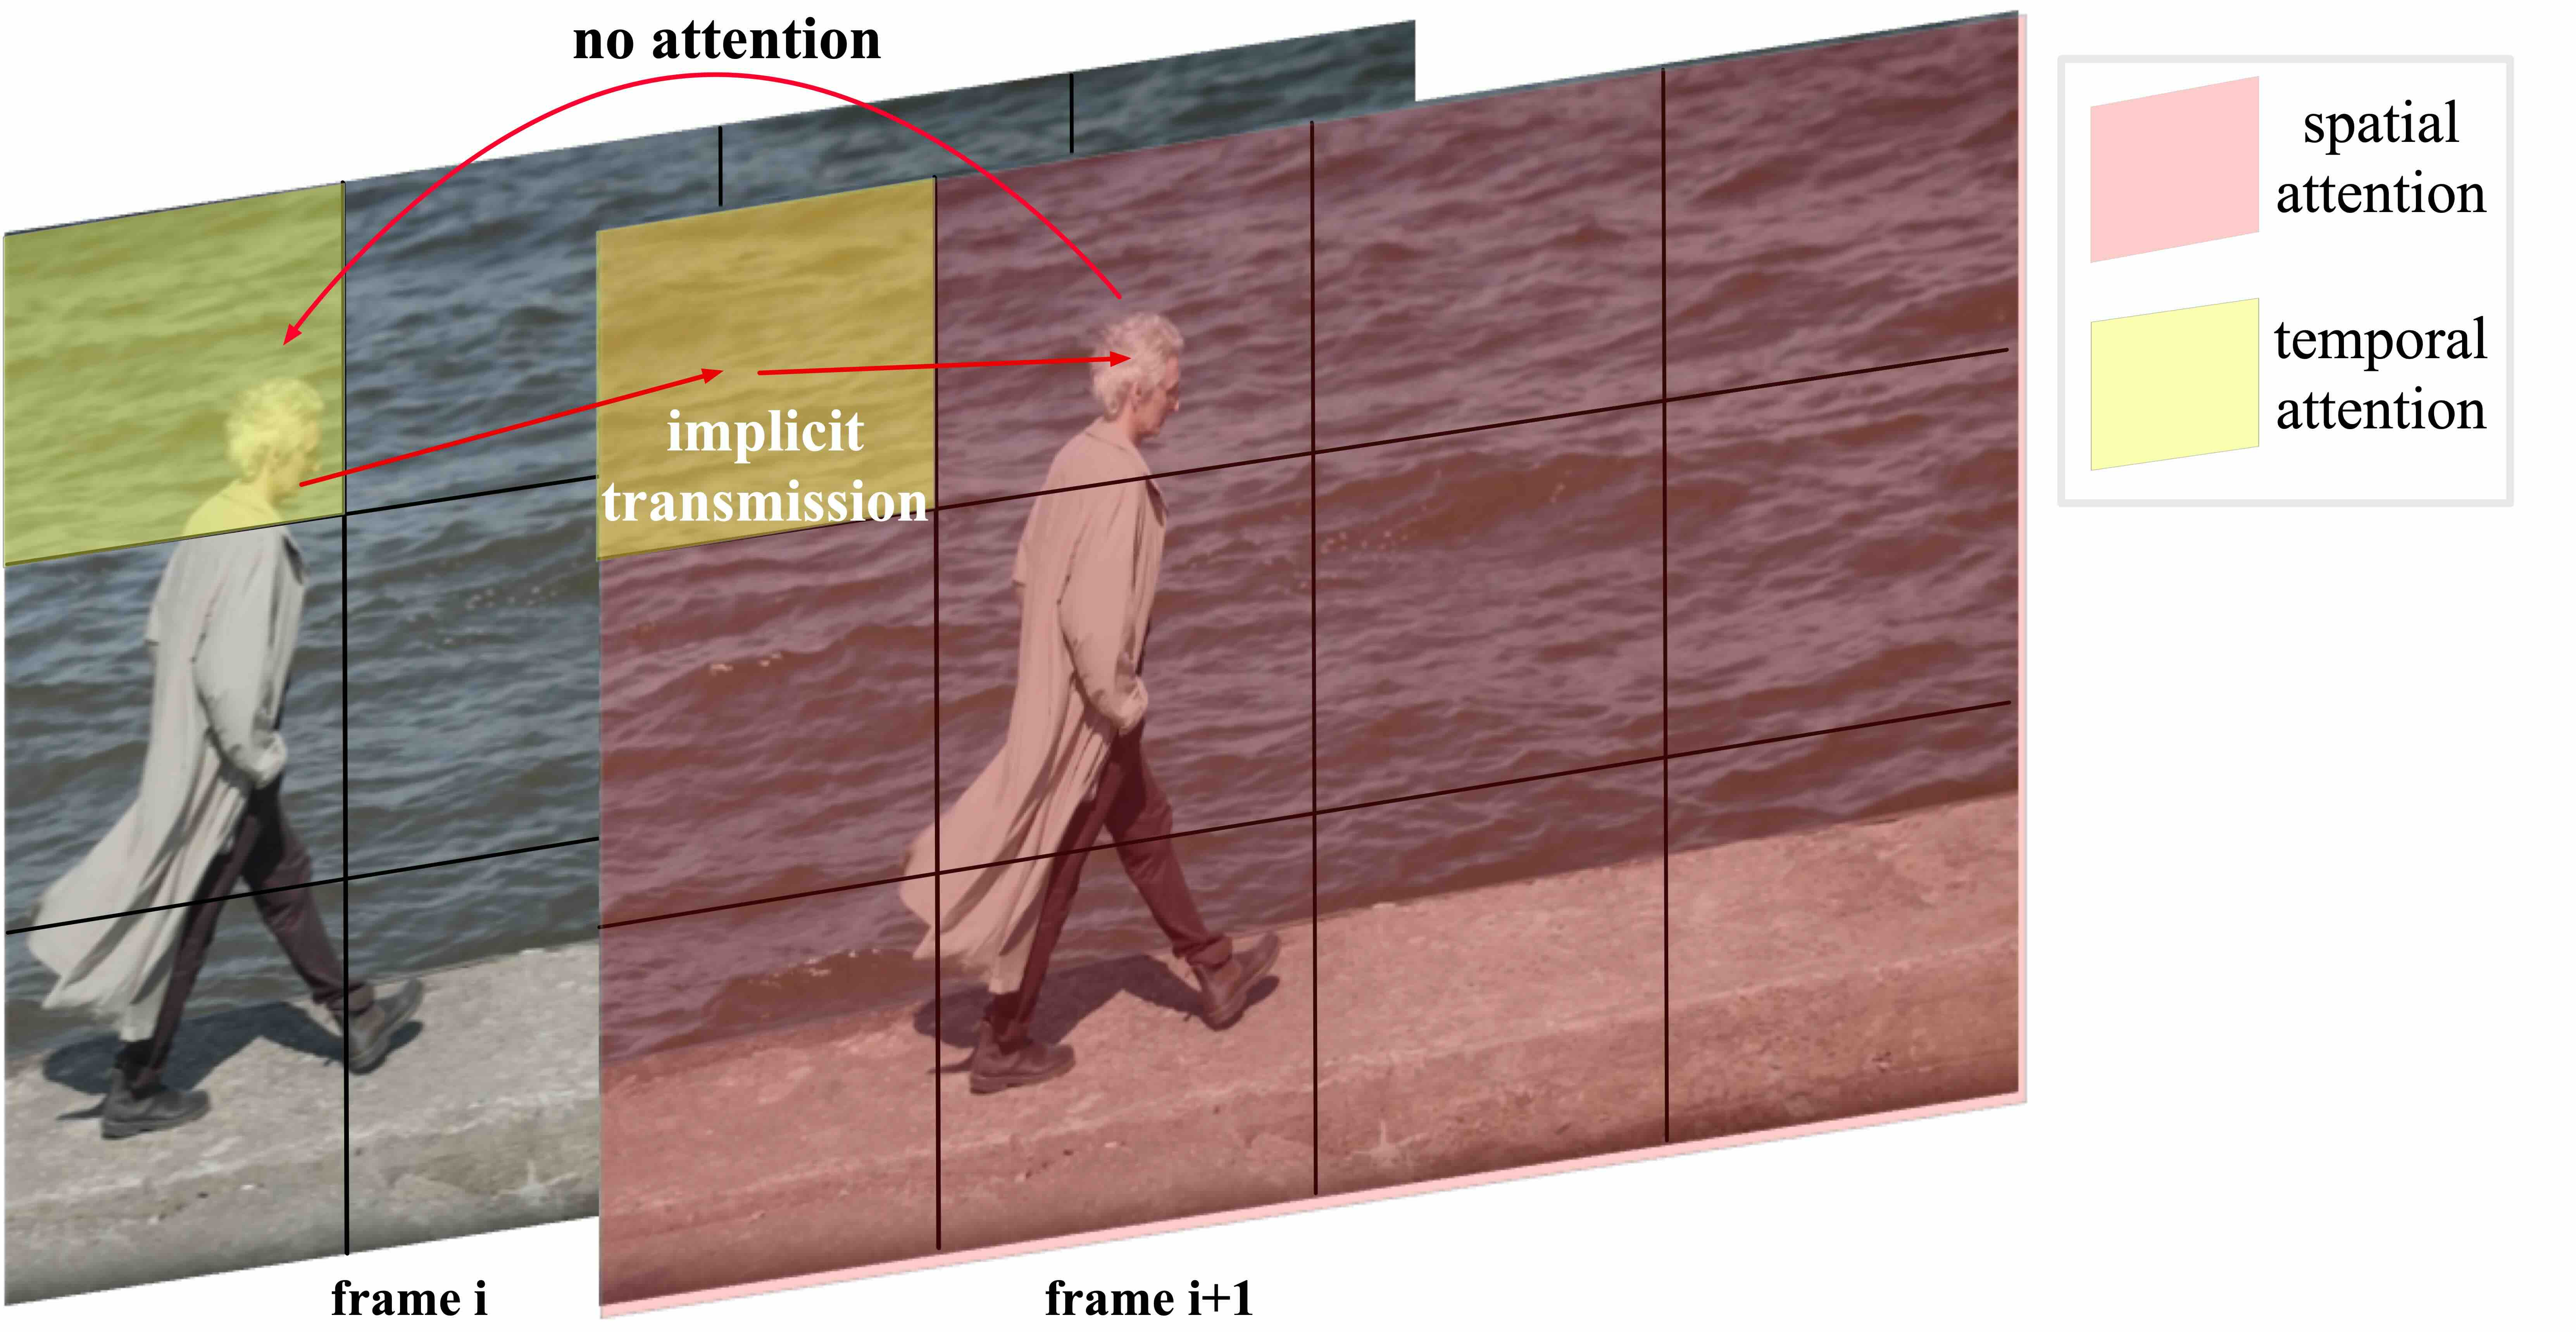
\includegraphics[width=\linewidth]{images/attention.png}
\caption{The separated spatial and temporal attention makes it challenging to handle the large motion between adjacent frames. In the figure, the head of the person in frame $i+1$ cannot directly attend to the head in the frame $i$. Instead, visual information can only be implicitly transmitted through other background patches. This can lead to inconsistency issues in the generated videos.}
\label{fig:attention}
\vspace{-10mm}
\end{wrapfigure}
}



 \subsection{Data}


We construct a collection of relatively high-quality video clips with text descriptions through video filters and recaption models. After filtering, approximately 35M single-shot clips remain, with each clip averaging about 6 seconds. 



\paragraph{Video Filtering.}
Video generation models need to learn the dynamic information of the world, but unfiltered video data is of highly noisy distribution, primarily due to two reasons: 
First, videos are human-created, and artificial editing may distort the authentic dynamic information; 
Second, the quality of videos can significantly drop due to issues during filming, such as camera shakes and substandard equipment.

In addition to the intrinsic quality of the videos, we also consider how well the video data supports model training. 
Videos with minimal dynamic information or lacking connectivity in dynamic aspects are considered detrimental. 
Consequently, we have developed a set of negative labels, which include:

\begin{itemize}
    \item \textbf{Editing}: Videos that have undergone obvious artificial processing, such as re-editing and special effects, causing degradation of the visual integrity.
    \item \textbf{Lack of Motion Connectivity}: Video segments with image transitions lacking motion connectivity, commonly seen in videos artificially spliced or edited from images.
    \item \textbf{Low Quality}: Poorly shot videos with unclear visuals or excessive camera shake.
    \item \textbf{Lecture Type}: Videos focusing primarily on a person continuously talking with minimal effective motion, such as educational content, lectures, and live-streamed discussions.
    \item \textbf{Text Dominated}: Videos containing a substantial amount of visible text or primarily focusing on textual content.
    \item \textbf{Noisy Screenshots}: Noisy videos recorded from phone or computer screens.
\end{itemize}

We sample 20,000 video data samples and label the presence of negative tags in each of them. 
By using these annotations, we train several filters based on video-llama~\cite{zhang2023video}  to screen out low-quality video data. 


In addition, we calculate the optical flow scores and image aesthetic scores of all training videos and dynamically adjust the threshold ranges during training  to ensure the fluency and aesthetic quality of the generated videos. 




\paragraph{Video Caption.} 
Typically, most video data does not come with corresponding descriptive text, so it is necessary to convert the video data into textual descriptions to provide the essential training data for text-to-video models. 
Currently, there are some video caption datasets available, such as Panda70M~\cite{chen2024panda}, COCO Caption~\cite{lin2014microsoft}, and WebVid~\cite{bain2021frozen}. 
However, the captions in these datasets are usually very short and fail to describe the video's content comprehensively. 




\begin{figure}[h]
\begin{center}
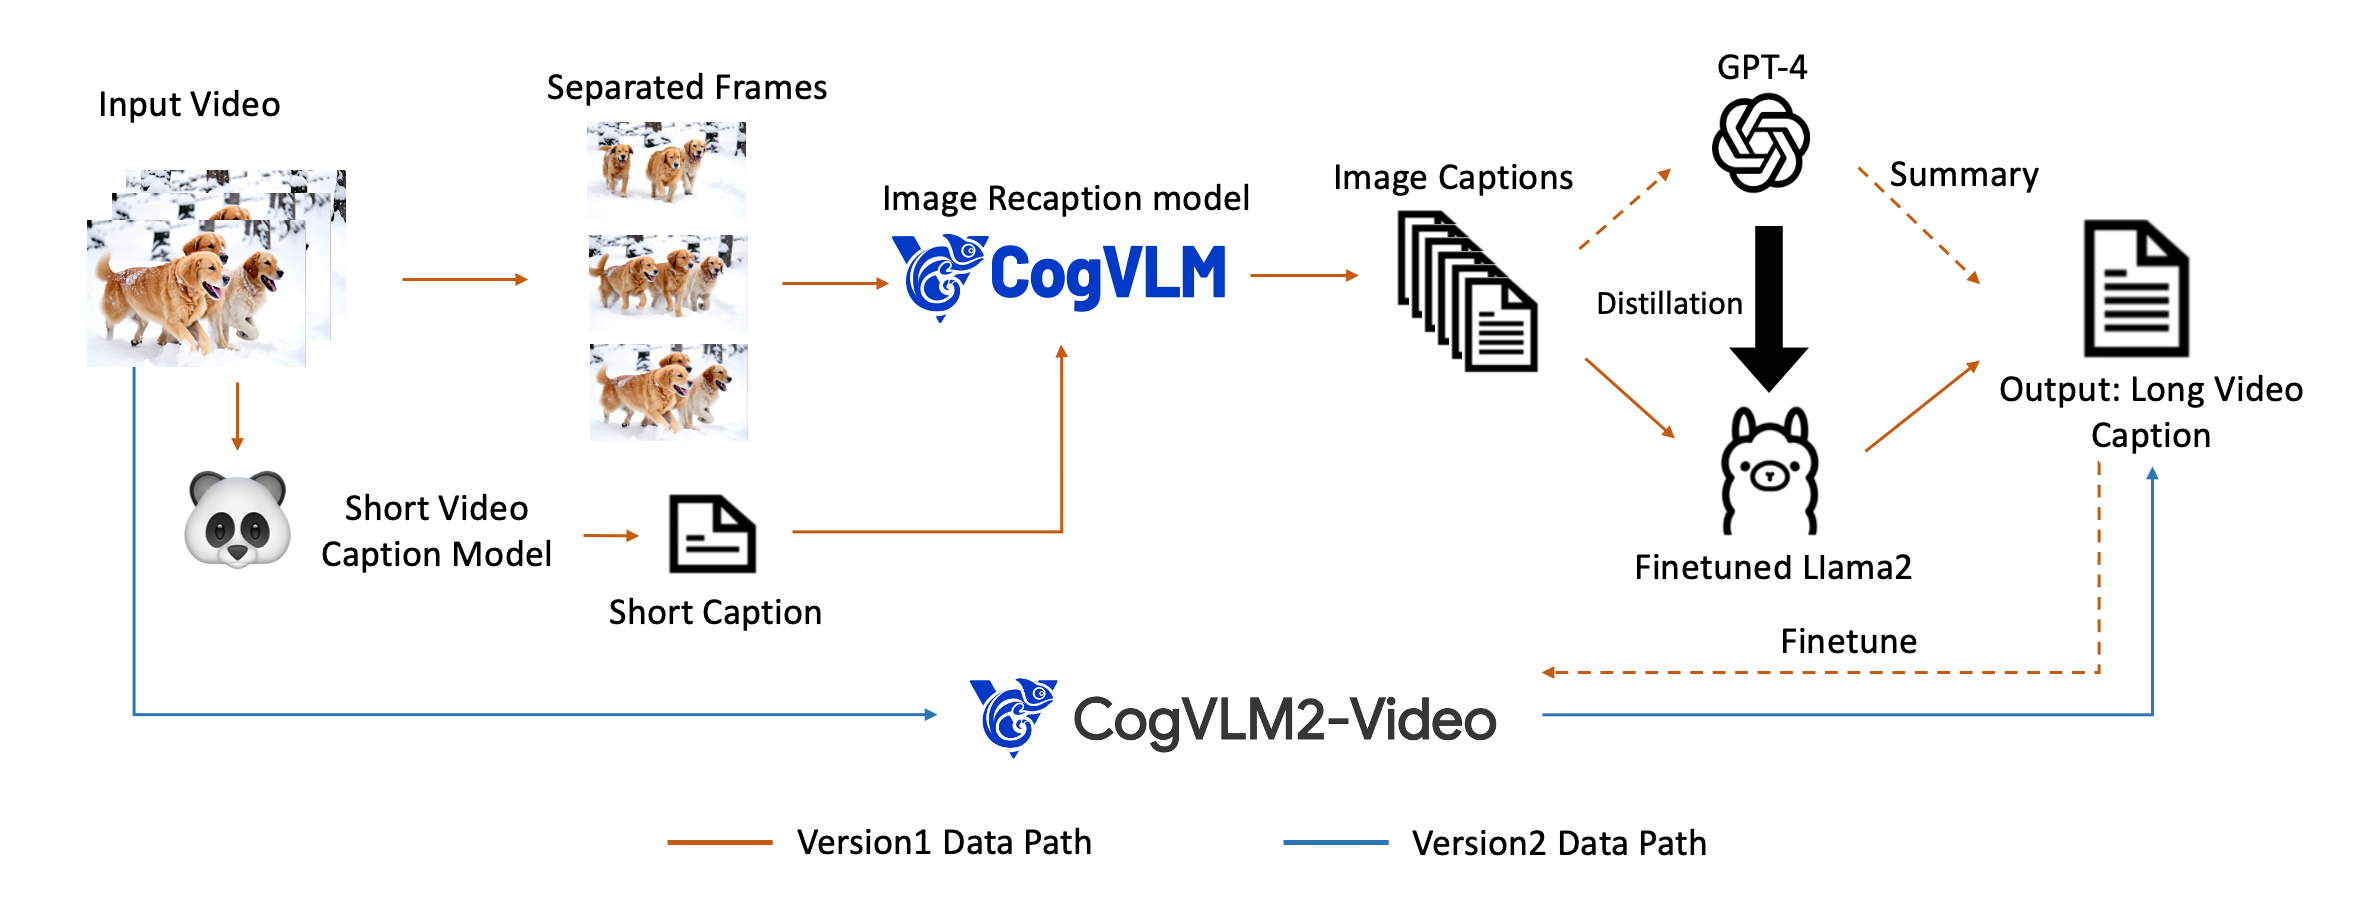
\includegraphics[width=\linewidth]{images/pipeline.jpg}
\end{center}
\caption{The pipeline for dense video caption data generation. In this pipeline, we generate short video captions with the Panda70M model, extract frames to create dense image captions, and use GPT-4 to summarize these into final video captions. To accelerate this process, we fine-tuned a Llama 2 model with the GPT-4 summaries.}
\label{fig:video_caption_gen}
\end{figure} 
To generate high-quality video caption data, we establish a \textit{Dense Video Caption Data Generation} 
pipeline, as detailed in Figure~\ref{fig:video_caption_gen}.  
The idea is to generate video captions from image captions. 

First, we use the Panda70M video captioning model~\cite{chen2024panda} to generate short captions for the videos. 
Then, we employ the image recaptioning model CogVLM~\cite{wang2023cogvlm} used in Stable~Diffusion~3~\cite{esser2024scaling} and CogView3~\cite{zheng2024cogview3} to create dense image captions for each of the frames within a video.  
Subsequently, we use GPT-4 to summarize all the image captions to produce the final video caption. 
To accelerate the generation from image captions to video captions, we fine-tune a Llama2 model~\cite{touvron2023llama} using the summary data generated by GPT-4~\cite{GPT4}, enabling large-scale video caption data generation. Additional details regarding the video caption data generation process can be found in Appendix~\ref{ap:video_caption_gen}.




The pipeline above generates the caption data that is used to trained the \model model introduced in this report. 
To further accelerate video recaptioning, we also fine-tune an end-to-end video understanding model CogVLM2-Caption, based on the CogVLM2-Video\footnote{The CogVLM2-Video model weight is openly available at \url{https://github.com/THUDM/CogVLM2}.} and Llama3~\cite{llama3modelcard}, by using the dense caption data generated from the aforementioned pipeline. 
The video caption data generated by CogVLM2-Caption is used to train the next generation of \model. 
Examples of video captions generated by this end-to-end CogVLM2-Caption model are shown in Appendix~\ref{ap:video_caption_example}. 
In Appendix~\ref{ap:v2v}, we also present some examples of video generation where a video is first input into CogVLM2-Caption to generate captions, which are then used as input for \model to generate new videos, effectively achieving video-to-video generation.



 \begin{figure}[ht]
\begin{center}
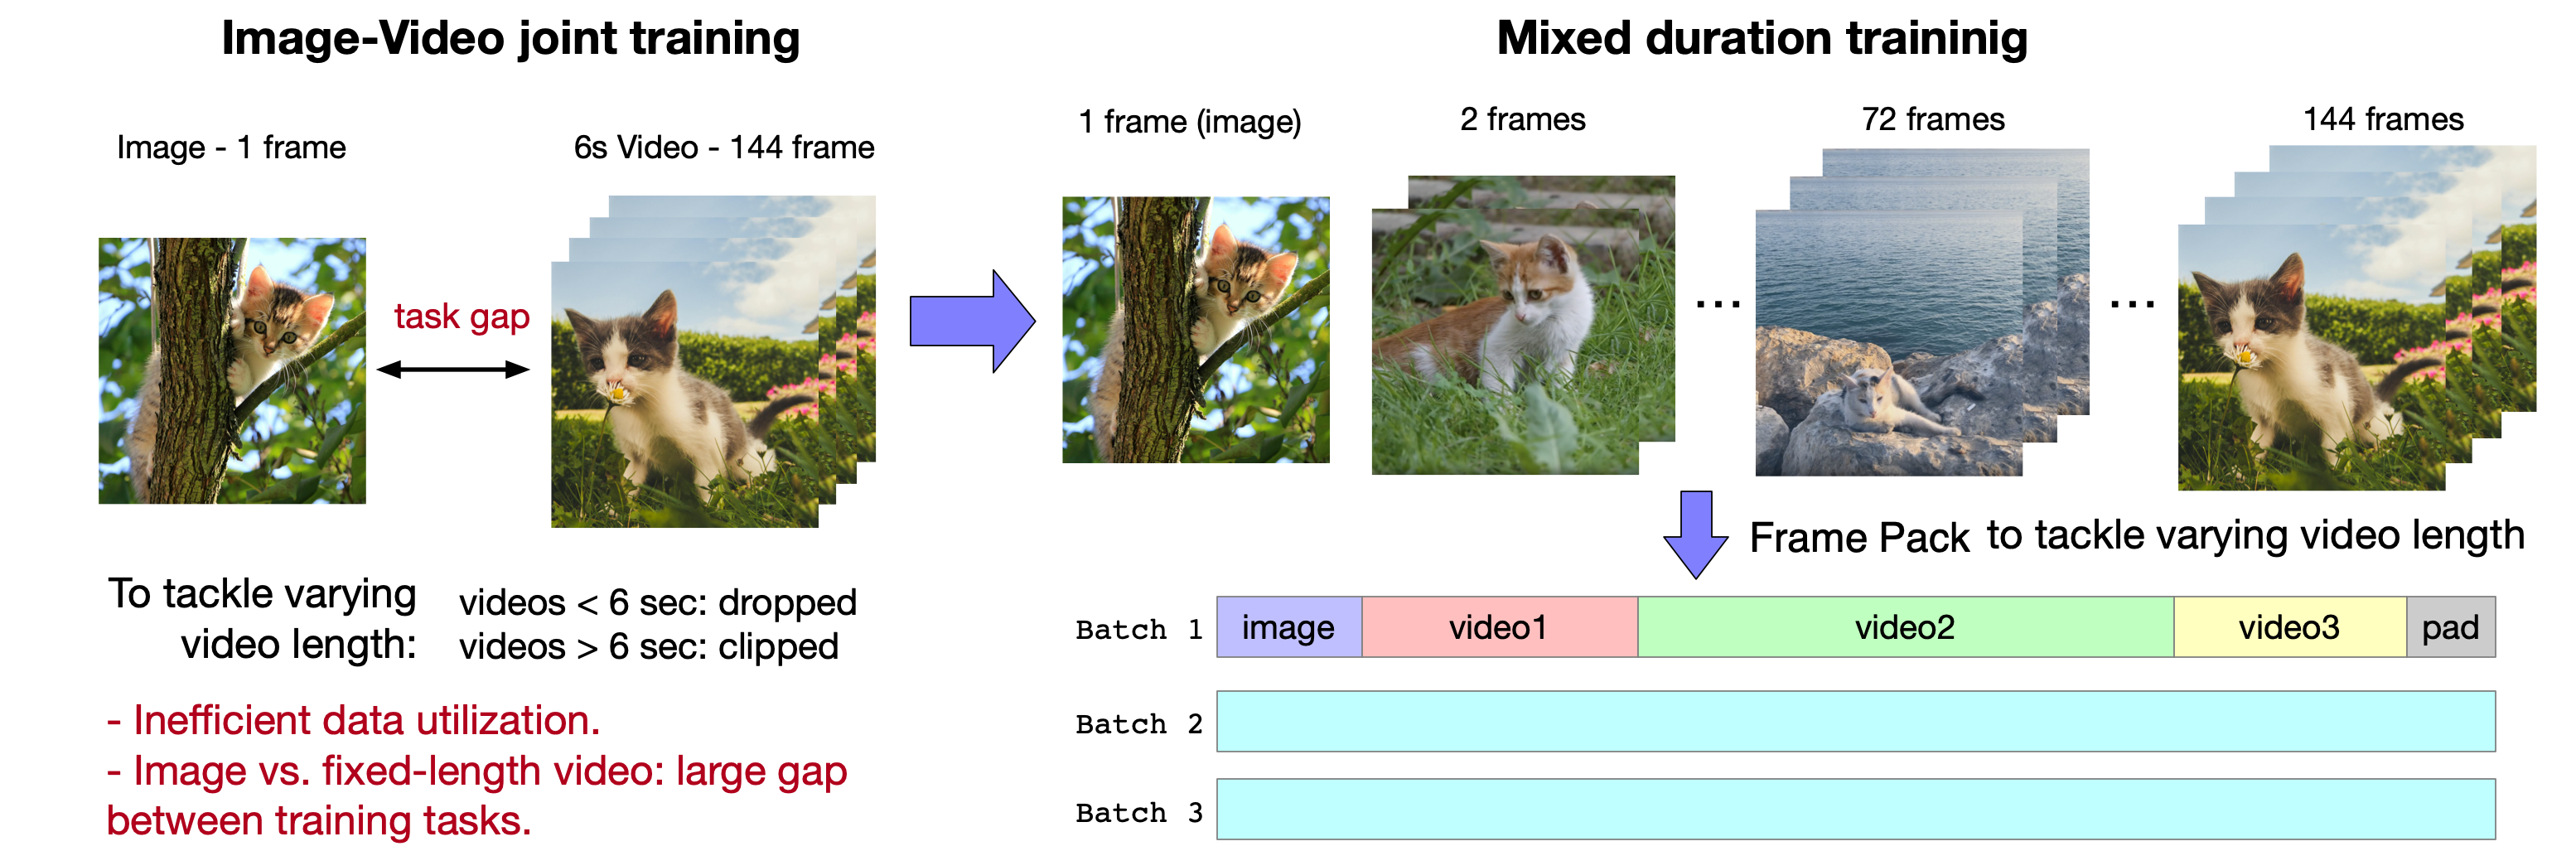
\includegraphics[width=\linewidth]{images/CogVideoX.png}
\end{center}
\caption{
The diagram of mixed-duration training and Frame Pack. To fully utilize the data and enhance the model's generalization capability, we train with videos of different durations within the same batch.}
\label{fig:framepack}
\end{figure}

\section{Training \model}

We mix images and videos during training, treating each image as a single-frame video. 
Additionally, we employ progressive training from the resolution perspective. 
For the diffusion setting, we adopt v-prediction~\cite{salimans2022progressive} and zero SNR~\cite{lin2024common}, following the noise schedule used in LDM~\cite{rombach2022high}.
During diffusion training for timestep sampling, we also employ an explicit uniform timestep sampling method, which benefits training stability. 

\subsection{Frame Pack}
Previous video training methods often involve joint training of images and videos with fixed number of frames~\cite{singer2022make, blattmann2023stable}. 
However, this approach usually leads to two issues: 
First, there is a significant gap between the two input types using bidirectional attention, with images having one frame while videos having dozens of frames. 
We observe that models trained this way tend to diverge into two generative modes based on the token count and not to have good generalizations. Second, to train with a fixed duration, we have to discard short videos and truncate long videos, which prevents full utilization of the videos of varying number of frames.

To address these issues, we choose mixed-duration training, which means training videos of different lengths together. 
However, inconsistent data shapes within the batch make training difficult. 
Inspired by Patch'n Pack \cite{dehghani2024patch}, we place videos of different lengths into the same batch to ensure consistent shapes within each batch, a method we refer to as \textit{Frame Pack}. The process is illustrated in Figure~\ref{fig:framepack}. 

\subsection{Resolution Progressive Training}

The training pipeline of \model is divided into three stages: low-resolution training, high-resolution training, and high-quality video fine-tuning. 
Similar to images, videos from the Internet usually include a significant amount of low-resolution ones. 
Progressive training can effectively utilize videos of various resolutions. 
Moreover, training at low resolution initially can equip the model with coarse-grained modeling capabilities, followed by high-resolution training to enhance its ability to capture fine details. 
Compared to direct high-resolution training, staged training can also help reduce the overall training time.

\begin{figure}[h]
\begin{center}
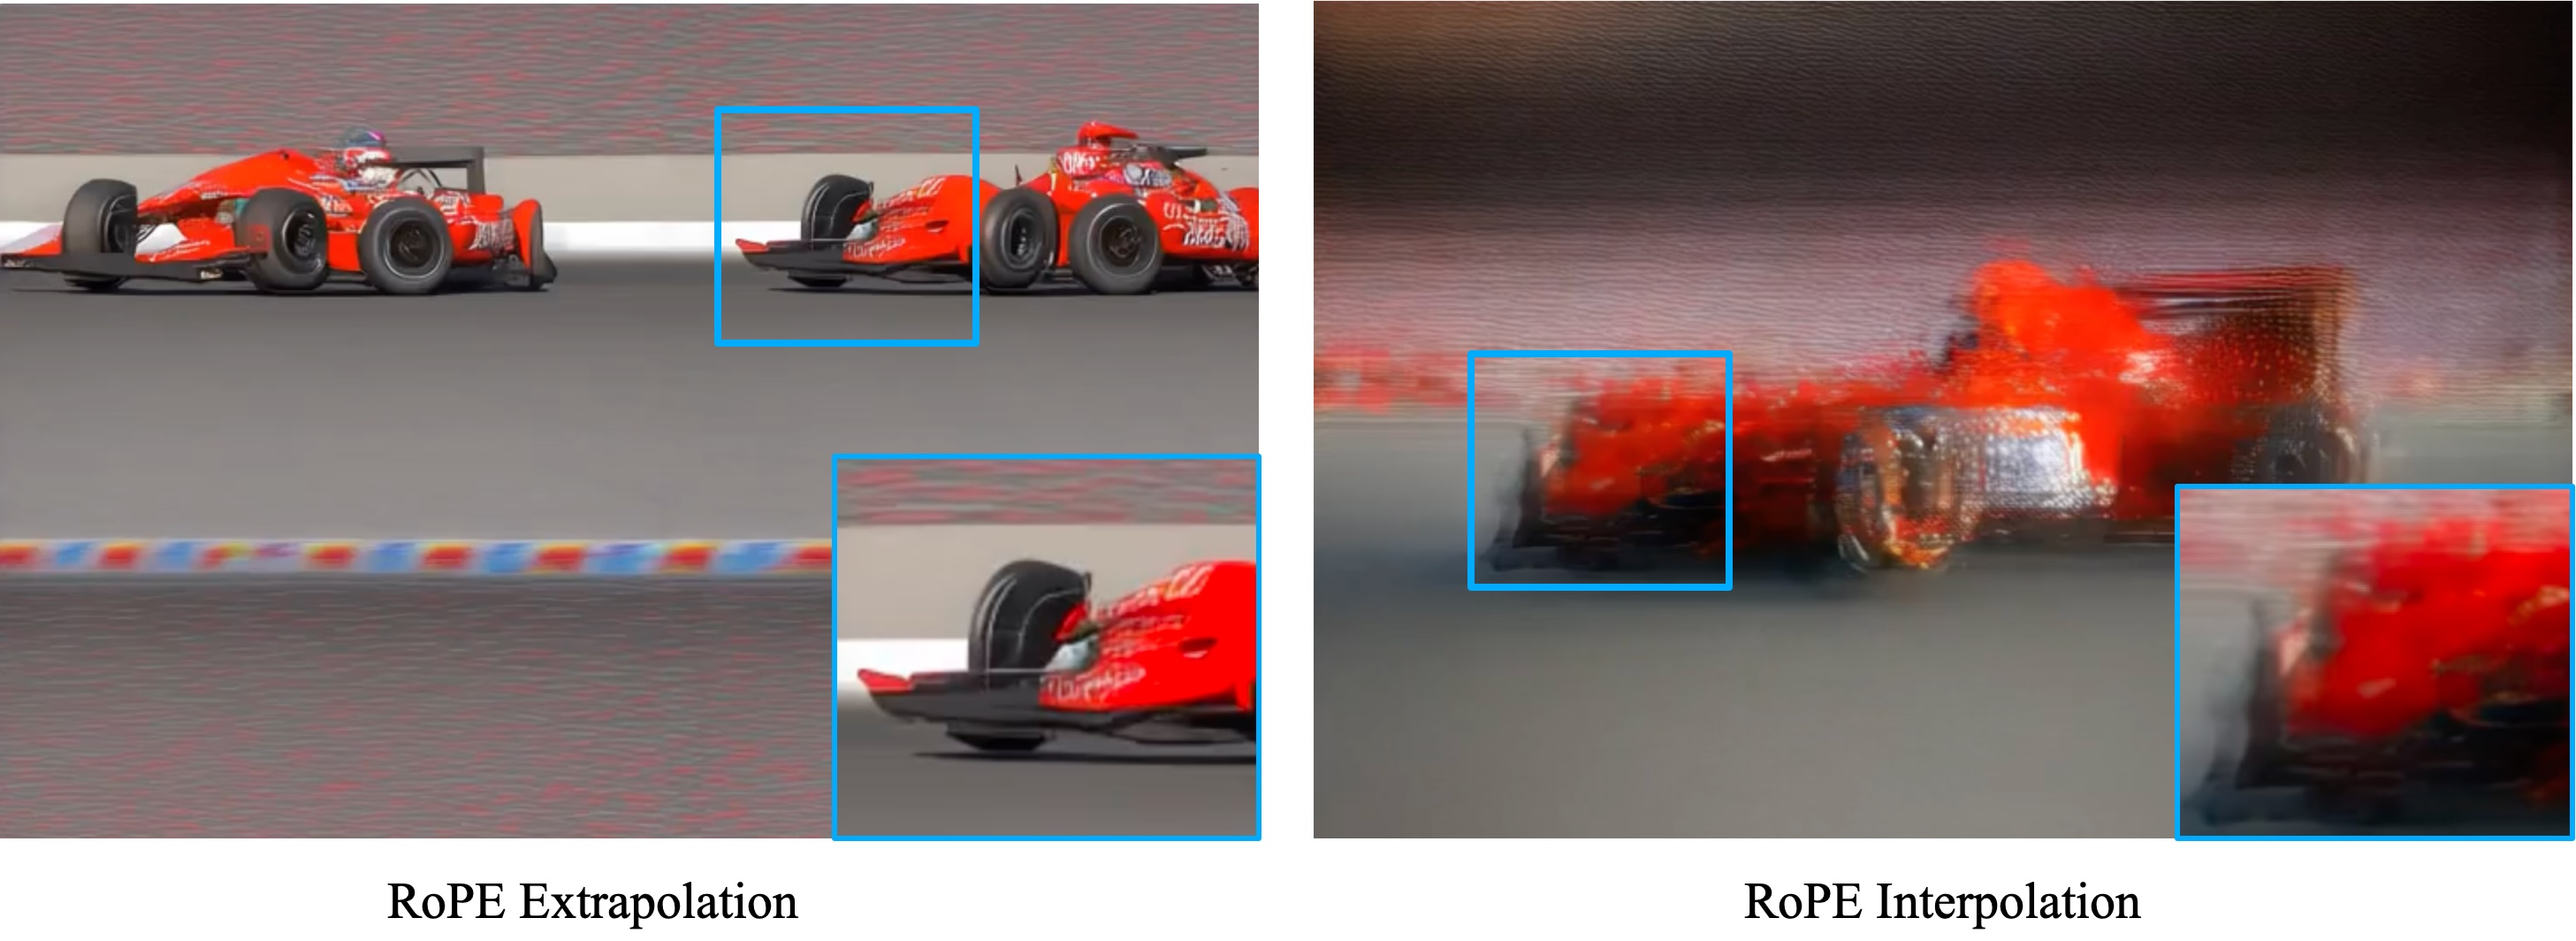
\includegraphics[width=0.9\linewidth]{images/ive.jpg}
\end{center}
\caption{The comparison between the initial generation states of extrapolation and interpolation when increasing the resolution with RoPE encoding. Extrapolation tends to generate multiple small, clear, and repetitive images, while interpolation generates a blurry large image.}
\label{fig:ive}
\end{figure}

\paragraph{Extrapolation of Position Code.}
When adapting low-resolution position encoding to high-resolution, we consider two different methods: interpolation and extrapolation. We show the effects of two methods in Figure~\ref{fig:ive}. Interpolation tens to preserve global information more effectively, whereas the extrapolation better retains local details. Given that RoPE is a relative position encoding, We chose the extrapolation to maintain the relative position between pixels. 

\paragraph{High-Quality Fine-Tuning.}
Since the filtered pre-training data still contains a certain proportion of dirty data, such as subtitles, watermarks, and low-bitrate videos, we selected a subset of higher quality video data, accounting for 20\% of the total dataset, for fine-tuning in the final stage. This step effectively removed generated subtitles and watermarks and slightly improved the visual quality. However, we also observed a slight degradation in the model's semantic ability.


\subsection{Explicit Uniform Sampling}

~\cite{ho2020denoising} defines the training objective of diffusion as 
\begin{equation}~\label{eq:ddpm-loss}
    L_\mathrm{simple}(\theta) := \mathbf{E}_{t, x_0, \epsilon}{ \left\| \epsilon - \epsilon_\theta(\sqrt{\bar\alpha_t} x_0 + \sqrt{1-\bar\alpha_t}\epsilon, t) \right\|^2},
\end{equation}
where $t$ is uniformly distributed between 1 and T. 
The common practice is for each rank in the data parallel group to uniformly sample a value between 1 and $T$, which is in theory equivalent to Equation~\ref{eq:ddpm-loss}. 
However, in practice, the results obtained from such random sampling are often not sufficiently uniform, and since the magnitude of the diffusion loss is related to the timesteps, this can lead to significant fluctuations in the loss. 
Thus, we propose to use \textit{Explicit Uniform Sampling} to divide the range from 1 to $T$ into $n$ intervals, where $n$ is the number of ranks. 
Each rank then uniformly samples within its respective interval. 
This method ensures a more uniform distribution of timesteps. 
As shown in Figure~\ref{fig:subfigures} (d), the loss curve from training with Explicit Uniform Sampling is noticeably more stable. 

In addition, we compare the loss at each diffusion timestep alone between the two methods for a more precise comparison. We find that after using explicit uniform sampling, the loss at all timesteps decreased faster, indicating that this method can accelerate loss convergence. 

We conducted ablation studies on some of the designs mentioned in Section~\ref{sec:model} to verify their effectiveness.


\subsection{Position Embedding}
First, we compared 3D RoPE with sinusoidal absolute position encoding. As shown in Figure~\ref{fig:d}, the loss curve using 3D RoPE converges significantly faster than that with sinusoidal encoding.
Then we compared the use of 3D RoPE alone with the combination of 3D RoPE and learnable absolute position embedding. As shown in Figure~\ref{fig:c}, the loss curves of both methods converge almost identically. For simplicity, we chose to use 3D RoPE alone.

\subsection{Expert Adaptive Layernorm}
We experimented with different ways of incorporating experts: expert LayerNorm and MLP, and expert Layernorm only. Our experiments found that adding expert MLP does not effectively accelerate the model's convergence (Figure~\ref{fig:b}). To reduce the model parameters, we only chose to use expert adaptive Layernorm. \section{Empirical Evaluation}

In this section, we present the performance of \model through two primary methods: \textit{automated metric evaluation} and \textit{human assessment}. We train the \model models with different parameter sizes. 
We show results for 2B and 5B for now, larger models are still in training.


To facilitate the development of text-to-video generation, we open-source the model weight at \url{https://github.com/THUDM/CogVideo}.




\subsection{Automated Metric Evaluation} 

\paragraph{Baselines.} 
We choose openly-accessible top-performing text-to-video models as baselines, including T2V-Turbo~\cite{li2024t2v}, AnimateDiff~\cite{guo2023animatediff}, VideoCrafter2~\cite{chen2024videocrafter2}, OpenSora~\cite{opensora}, Show-1~\cite{zhang2023show}, Gen-2~\cite{gen2}, Pika~\cite{pika}, and LaVie-2~\cite{wang2023lavie}.




\hide{
\begin{figure}
\centering
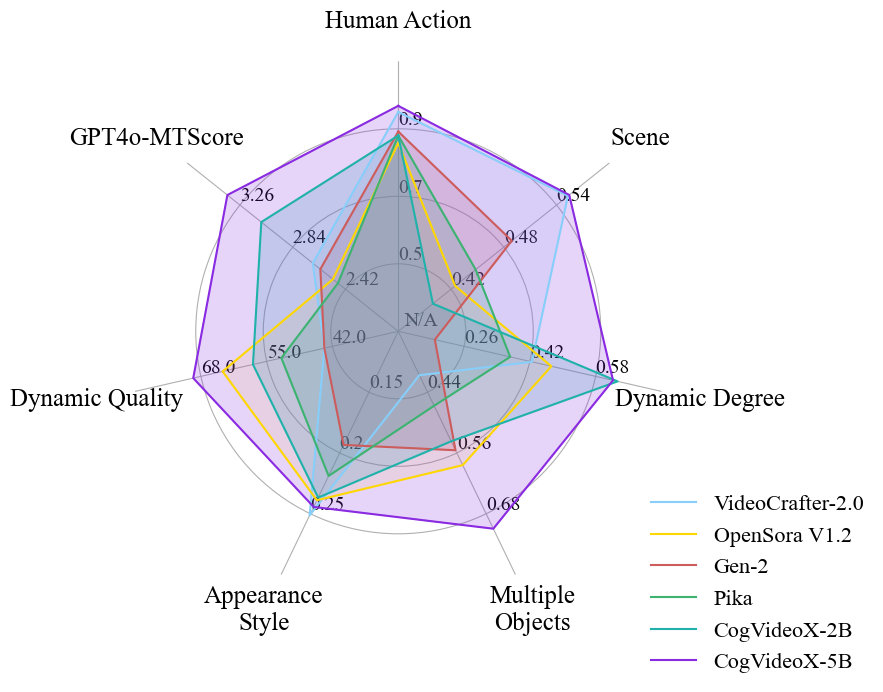
\includegraphics[width=0.7\linewidth]{images/bench_eval9.png}
\caption{The radar chart comparing the performance of different models. CogVideoX represents the largest one. It is clear that CogVideoX outperforms its competitors in the vast majority of metrics, and it is very close to the leading models in the remaining indicator.
}
\label{fig:radar}


\end{figure}

}%
 
\paragraph{Evaluation Metrics.} 
To evaluate the text-to-video generation, we employed several metrics from VBench~\cite{huang2023vbench}: \emph{Human Action}, \emph{Scene}, \emph{Dynamic Degree}, \emph{Multiple Objects}, and \emph{Appearance Style}. 
VBench is a suite of tools designed to automatically assess the quality of generated videos. We have selected certain metrics from VBench, excluding others that do not align with our evaluation needs. 
For example, the color metric, intended to measure the presence of objects corresponding to specific colors across frames in the generated video, assesses the model's quality by calculating the probability. 
However, this metric may mislead video generation models that exhibit greater variation, thus it is not to include it in our evaluation. 

For longer-generated videos, some models might produce videos with minimal changes between frames to obtain higher scores, but these videos lack rich content. 
Therefore, a metric for evaluating the dynamism of the video becomes more important. 
To address this, we employ two video evaluation tools:  \emph{Dynamic Quality} from Devil~\cite{liao2024evaluationtexttovideogenerationmodels} and \emph{GPT4o-MTScore} from ChronoMagic~\cite{yuan2024chronomagic}, which focus more on the dynamic characteristics of videos. 
\emph{Dynamic Quality} is defined by the integration of various quality metrics with dynamic scores, mitigating biases arising from negative correlations between video dynamics and video quality.
ChronoMagic, for instance, introduces {GPT4o-MTScore}, a metric designed to measure the metamorphic amplitude of time-lapse videos, such as those depicting physical, biological, and meteorological changes. 
This metric using GPT-4o~\cite{gpt4o} to score the degree of change, providing a fine-grained assessment of video dynamism. 




\paragraph{Results.} 
Table~\ref{table:results} provides the performance comparison of \model and other models. 
\model achieves the best performance in five out of the seven metrics and shows competitive results in the remaining two metrics. 
These results demonstrate that the model not only excels in video generation quality but also outperforms previous models in handling various complex dynamic scenes. 
In addition, Figure~\ref{fig:radar} presents a radar chart that visually illustrates the performance advantages of \model.


\begin{figure}[ht]
\begin{center}
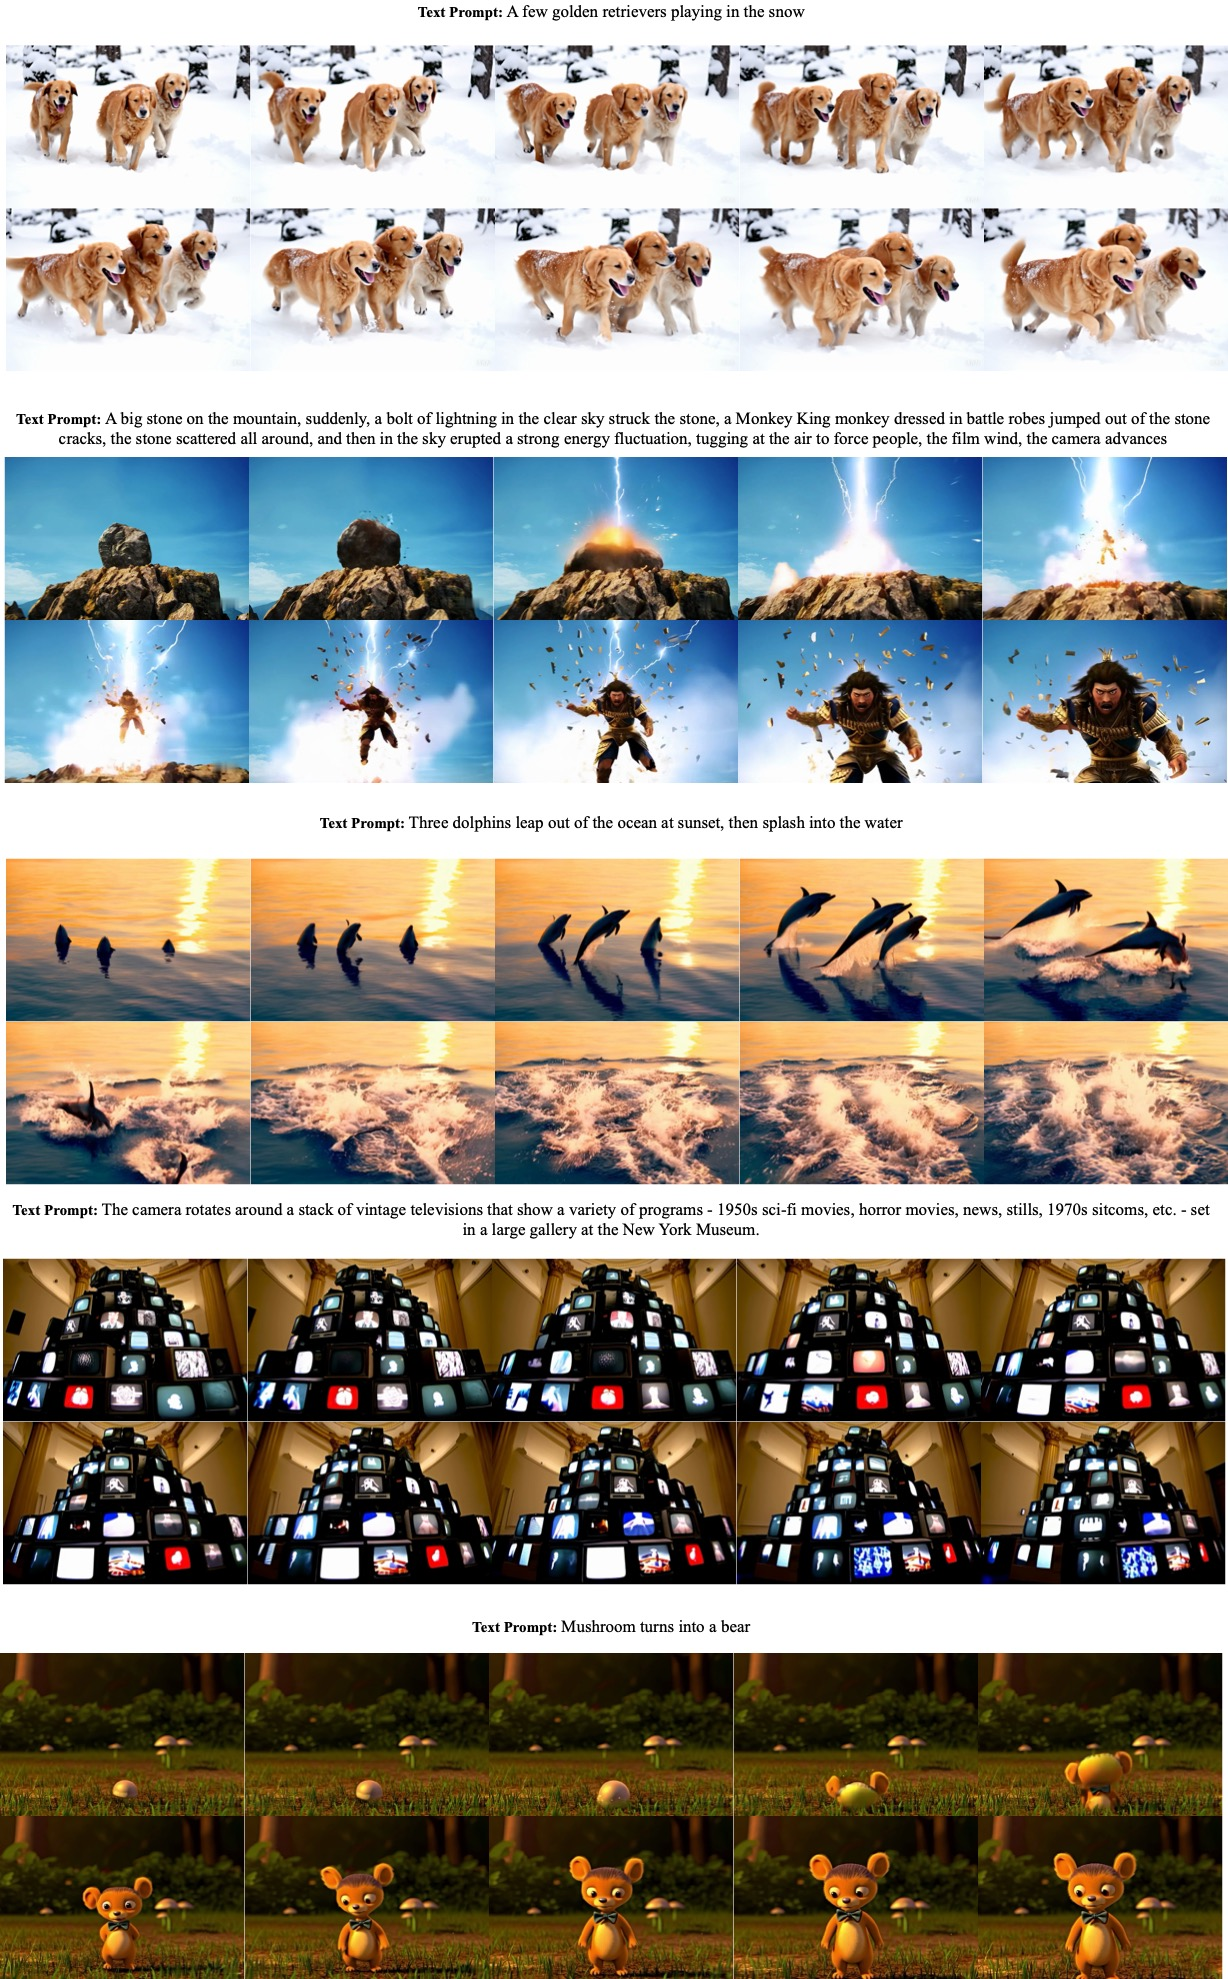
\includegraphics[width=\linewidth]{images/t2v/goodcase1.jpg}
\end{center}
\caption{Text to video showcases. The displayed prompt will be upsampled before being fed into the model. The generated videos contain large motion and can produce various video styles.}
\label{fig:t2vgood1}
\end{figure}

\begin{figure}[ht]
\begin{center}
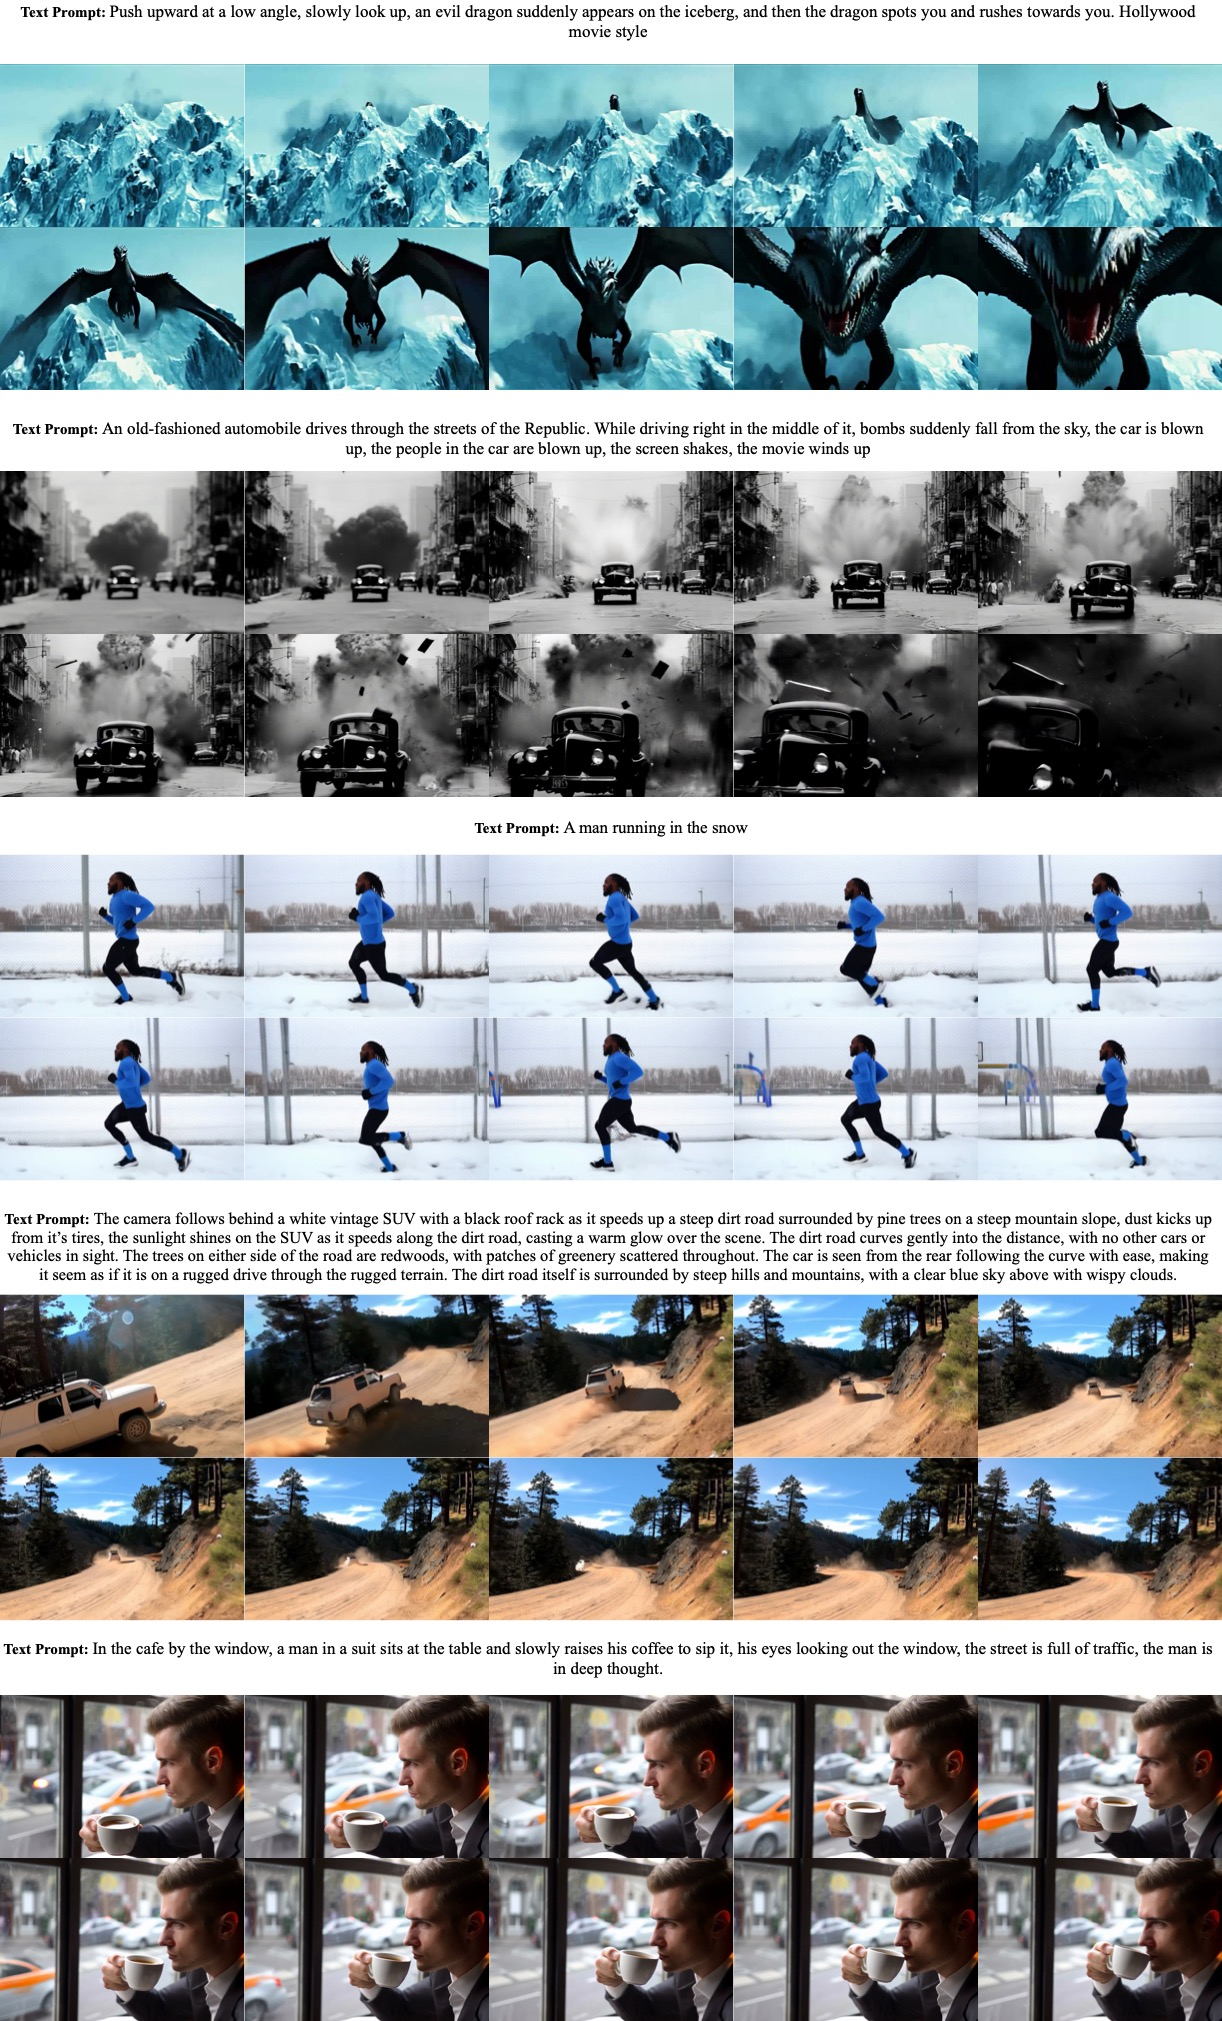
\includegraphics[width=0.98\linewidth]{images/t2v/goodcase2.jpg}
\end{center}
\caption{Text to video showcases.}
\label{fig:t2vgood2}
\end{figure}


















































\begin{table}[t]
\caption{Evaluation results.}
\label{table:results}
\vspace{6pt}
\footnotesize
    \centering
    \begin{tabular}{cccccccc}
   \toprule
        Models & \Centerstack{Human \\Action}   & Scene & \Centerstack{Dynamic \\Degree} & \Centerstack{Multiple \\Objects} & \Centerstack{Appearance \\Style} & \Centerstack{Dynamic \\Quality} & \Centerstack{GPT4o-MT \\Score}  \\ 
        \midrule
        T2V-Turbo & 95.2 & \textbf{55.58} & 49.17 & 54.65 & 24.42 & -- & --  \\ 
        AnimateDiff & 92.6  & 50.19 & 40.83 & 36.88 & 22.42 & -- & 2.62  \\ 
        VideoCrafter-2.0 & 95.0  & 55.29 & 42.50 & 40.66 & \textbf{25.13} & 43.6 & 2.68  \\ 
        OpenSora V1.2 & 85.8  & 42.47 & 47.22 & 58.41  & 23.89 & 63.7 & 2.52  \\ 
        Show-1 & 95.6  & 47.03 & 44.44 & 45.47  & 23.06 & 57.7 & --  \\ 
        Gen-2 & 89.2  & 48.91 & 18.89 & 55.47 & 19.34 & 43.6 & 2.62  \\ 
        Pika & 88.0  & 44.80 & 37.22 & 46.69  & 21.89 & 52.1 & 2.48  \\ 
        LaVie-2 & 96.4 & 49.59 & 31.11 & 64.88  & 25.09 & -- & 2.46  \\ 
        \hline
        \textbf{CogVideoX-2B} & 88.0 & 39.94 & \textbf{63.33} & 53.70 & 23.67 & 57.7 & 3.09 \\
        \textbf{CogVideoX-5B} & \textbf{96.8} & 55.44 & 62.22 & \textbf{70.95} & 24.44 & \textbf{69.5} & \textbf{3.36} \\
        \bottomrule
    \end{tabular}
\end{table} 

\subsection{Human Evaluation}
In addition to automated scoring mechanisms, a comparative analysis between the Kling~\cite{kling} and CogVideoX is conducted with manual evaluation. 
One hundred meticulously crafted prompts are used for human evaluators, characterized by their broad distribution, clear articulation, and well-defined conceptual scope. 
We randomize videos for blind evalution. 
A panel of evaluators is instructed to assign scores for each detail on a scale from zero to one, with the overall total score rated on a scale from $0$ to $5$, where higher scores reflect better video quality. 
To better complement automated evaluation, human evaluation emphasizes the instruction-following capability: the total score cannot exceed $2$ if the generated video fails to follow the instruction.

The results shown in Table~\ref{table:human_eva} indicate that \model wins the human preference over Kling across all aspects. 
More details about human evaluation are shown in Appendix~\ref{sec:human_evalution}.

\begin{table}[!ht]
\centering
\label{sample-table}
\small
\vspace{-5pt}
\caption{Human evaluation between CogVideoX and Kling.}
\label{table:human_eva}
\resizebox{0.75\linewidth}{!}{
    \begin{tabular}{cccccc}
    \toprule
        Model & \Centerstack{Sensory\\Quality} & \Centerstack{Instruction\\Following}&\Centerstack{Physics\\Simulation} & \Centerstack{Cover\\Quality} & 
        \Centerstack{Total\\Score} \\ 
        \midrule
        Kling & 0.638 & 0.367 & 0.561 & 0.668 & 2.17 \\
        \midrule
         {\bf CogVideoX-5B} & {\bf 0.722} & {\bf 0.495} & {\bf 0.667} & {\bf 0.712} & {\bf 2.74}  \\
        \bottomrule
    \end{tabular}
}
\end{table} 








 
 
\subsubsection*{Acknowledgments}


We would like to thank all the data annotators, infra operating staffs, collaborators, and partners as well as everyone at Zhipu AI and Tsinghua University not explicitly mentioned in the report who have provided support, feedback, and contributed to \model. 
We would also like to greatly thank BiliBili for data support. 




\begin{thebibliography}{45}
\providecommand{\natexlab}[1]{#1}
\providecommand{\url}[1]{\texttt{#1}}
\expandafter\ifx\csname urlstyle\endcsname\relax
  \providecommand{\doi}[1]{doi: #1}\else
  \providecommand{\doi}{doi: \begingroup \urlstyle{rm}\Url}\fi

\bibitem{pika}
Pika beta.
\newblock 2023.
\newblock URL \url{https://pika.art/home}.

\bibitem{GPT4}
Josh Achiam, Steven Adler, Sandhini Agarwal, Lama Ahmad, Ilge Akkaya, Florencia~Leoni Aleman, Diogo Almeida, Janko Altenschmidt, Sam Altman, Shyamal Anadkat, et~al.
\newblock Gpt-4 technical report.
\newblock \emph{arXiv preprint arXiv:2303.08774}, 2023.

\bibitem{llama3modelcard}
AI@Meta.
\newblock Llama 3 model card.
\newblock 2024.
\newblock URL \url{https://github.com/meta-llama/llama3/blob/main/MODEL_CARD.md}.

\bibitem{bai2024longalign}
Yushi Bai, Xin Lv, Jiajie Zhang, Yuze He, Ji~Qi, Lei Hou, Jie Tang, Yuxiao Dong, and Juanzi Li.
\newblock Longalign: A recipe for long context alignment of large language models.
\newblock \emph{arXiv preprint arXiv:2401.18058}, 2024.

\bibitem{bain2021frozen}
Max Bain, Arsha Nagrani, G{\"u}l Varol, and Andrew Zisserman.
\newblock Frozen in time: A joint video and image encoder for end-to-end retrieval.
\newblock In \emph{Proceedings of the IEEE/CVF international conference on computer vision}, pp.\  1728--1738, 2021.

\bibitem{betker2023improving}
James Betker, Gabriel Goh, Li~Jing, Tim Brooks, Jianfeng Wang, Linjie Li, Long Ouyang, Juntang Zhuang, Joyce Lee, Yufei Guo, et~al.
\newblock Improving image generation with better captions.
\newblock \emph{Computer Science. https://cdn. openai. com/papers/dall-e-3. pdf}, 2\penalty0 (3):\penalty0 8, 2023.

\bibitem{blattmann2023stable}
Andreas Blattmann, Tim Dockhorn, Sumith Kulal, Daniel Mendelevitch, Maciej Kilian, Dominik Lorenz, Yam Levi, Zion English, Vikram Voleti, Adam Letts, et~al.
\newblock Stable video diffusion: Scaling latent video diffusion models to large datasets.
\newblock \emph{arXiv preprint arXiv:2311.15127}, 2023.

\bibitem{chen2024videocrafter2}
Haoxin Chen, Yong Zhang, Xiaodong Cun, Menghan Xia, Xintao Wang, Chao Weng, and Ying Shan.
\newblock Videocrafter2: Overcoming data limitations for high-quality video diffusion models, 2024{\natexlab{a}}.

\bibitem{chen2024panda}
Tsai-Shien Chen, Aliaksandr Siarohin, Willi Menapace, Ekaterina Deyneka, Hsiang-wei Chao, Byung~Eun Jeon, Yuwei Fang, Hsin-Ying Lee, Jian Ren, Ming-Hsuan Yang, et~al.
\newblock Panda-70m: Captioning 70m videos with multiple cross-modality teachers.
\newblock In \emph{Proceedings of the IEEE/CVF Conference on Computer Vision and Pattern Recognition}, pp.\  13320--13331, 2024{\natexlab{b}}.

\bibitem{dao2022flashattention}
Tri Dao, Dan Fu, Stefano Ermon, Atri Rudra, and Christopher R{\'e}.
\newblock Flashattention: Fast and memory-efficient exact attention with io-awareness.
\newblock \emph{Advances in Neural Information Processing Systems}, 35:\penalty0 16344--16359, 2022.

\bibitem{dehghani2024patch}
Mostafa Dehghani, Basil Mustafa, Josip Djolonga, Jonathan Heek, Matthias Minderer, Mathilde Caron, Andreas Steiner, Joan Puigcerver, Robert Geirhos, Ibrahim~M Alabdulmohsin, et~al.
\newblock Patch n’pack: Navit, a vision transformer for any aspect ratio and resolution.
\newblock \emph{Advances in Neural Information Processing Systems}, 36, 2024.

\bibitem{esser2021taming}
Patrick Esser, Robin Rombach, and Bjorn Ommer.
\newblock Taming transformers for high-resolution image synthesis.
\newblock In \emph{Proceedings of the IEEE/CVF conference on computer vision and pattern recognition}, pp.\  12873--12883, 2021.

\bibitem{esser2024scaling}
Patrick Esser, Sumith Kulal, Andreas Blattmann, Rahim Entezari, Jonas M{\"u}ller, Harry Saini, Yam Levi, Dominik Lorenz, Axel Sauer, Frederic Boesel, et~al.
\newblock Scaling rectified flow transformers for high-resolution image synthesis.
\newblock In \emph{Forty-first International Conference on Machine Learning}, 2024.

\bibitem{guo2023animatediff}
Yuwei Guo, Ceyuan Yang, Anyi Rao, Zhengyang Liang, Yaohui Wang, Yu~Qiao, Maneesh Agrawala, Dahua Lin, and Bo~Dai.
\newblock Animatediff: Animate your personalized text-to-image diffusion models without specific tuning.
\newblock \emph{arXiv preprint arXiv:2307.04725}, 2023.

\bibitem{ho2020denoising}
Jonathan Ho, Ajay Jain, and Pieter Abbeel.
\newblock Denoising diffusion probabilistic models.
\newblock \emph{Advances in neural information processing systems}, 33:\penalty0 6840--6851, 2020.

\bibitem{ho2022imagen}
Jonathan Ho, William Chan, Chitwan Saharia, Jay Whang, Ruiqi Gao, Alexey Gritsenko, Diederik~P Kingma, Ben Poole, Mohammad Norouzi, David~J Fleet, et~al.
\newblock Imagen video: High definition video generation with diffusion models.
\newblock \emph{arXiv preprint arXiv:2210.02303}, 2022.

\bibitem{hong2022cogvideo}
Wenyi Hong, Ming Ding, Wendi Zheng, Xinghan Liu, and Jie Tang.
\newblock Cogvideo: Large-scale pretraining for text-to-video generation via transformers.
\newblock \emph{arXiv preprint arXiv:2205.15868}, 2022.

\bibitem{huang2023vbench}
Ziqi Huang, Yinan He, Jiashuo Yu, Fan Zhang, Chenyang Si, Yuming Jiang, Yuanhan Zhang, Tianxing Wu, Qingyang Jin, Nattapol Chanpaisit, Yaohui Wang, Xinyuan Chen, Limin Wang, Dahua Lin, Yu~Qiao, and Ziwei Liu.
\newblock {VBench}: Comprehensive benchmark suite for video generative models.
\newblock In \emph{Proceedings of the IEEE/CVF Conference on Computer Vision and Pattern Recognition}, 2024.

\bibitem{li2024t2v}
Jiachen Li, Weixi Feng, Tsu-Jui Fu, Xinyi Wang, Sugato Basu, Wenhu Chen, and William~Yang Wang.
\newblock T2v-turbo: Breaking the quality bottleneck of video consistency model with mixed reward feedback.
\newblock \emph{arXiv preprint arXiv:2405.18750}, 2024.

\bibitem{liao2024evaluationtexttovideogenerationmodels}
Mingxiang Liao, Hannan Lu, Xinyu Zhang, Fang Wan, Tianyu Wang, Yuzhong Zhao, Wangmeng Zuo, Qixiang Ye, and Jingdong Wang.
\newblock Evaluation of text-to-video generation models: A dynamics perspective, 2024.
\newblock URL \url{https://arxiv.org/abs/2407.01094}.

\bibitem{lin2024common}
Shanchuan Lin, Bingchen Liu, Jiashi Li, and Xiao Yang.
\newblock Common diffusion noise schedules and sample steps are flawed.
\newblock In \emph{Proceedings of the IEEE/CVF winter conference on applications of computer vision}, pp.\  5404--5411, 2024.

\bibitem{lin2014microsoft}
Tsung-Yi Lin, Michael Maire, Serge Belongie, James Hays, Pietro Perona, Deva Ramanan, Piotr Doll{\'a}r, and C~Lawrence Zitnick.
\newblock Microsoft coco: Common objects in context.
\newblock In \emph{Computer Vision--ECCV 2014: 13th European Conference, Zurich, Switzerland, September 6-12, 2014, Proceedings, Part V 13}, pp.\  740--755. Springer, 2014.

\bibitem{gpt4o}
OpenAI.
\newblock Gpt-4o.
\newblock 2024{\natexlab{a}}.

\bibitem{sora}
OpenAI.
\newblock Sora.
\newblock 2024{\natexlab{b}}.
\newblock URL \url{https://openai.com/index/sora/}.

\bibitem{peebles2023scalable}
William Peebles and Saining Xie.
\newblock Scalable diffusion models with transformers.
\newblock In \emph{Proceedings of the IEEE/CVF International Conference on Computer Vision}, pp.\  4195--4205, 2023.

\bibitem{raffel2020exploring}
Colin Raffel, Noam Shazeer, Adam Roberts, Katherine Lee, Sharan Narang, Michael Matena, Yanqi Zhou, Wei Li, and Peter~J Liu.
\newblock Exploring the limits of transfer learning with a unified text-to-text transformer.
\newblock \emph{Journal of machine learning research}, 21\penalty0 (140):\penalty0 1--67, 2020.

\bibitem{rombach2022high}
Robin Rombach, Andreas Blattmann, Dominik Lorenz, Patrick Esser, and Bj{\"o}rn Ommer.
\newblock High-resolution image synthesis with latent diffusion models.
\newblock In \emph{Proceedings of the IEEE/CVF conference on computer vision and pattern recognition}, pp.\  10684--10695, 2022.

\bibitem{gen2}
runway.
\newblock Gen-2.
\newblock 2023.
\newblock URL \url{https://runwayml.com/ai-tools/gen-2-text-to-video}.

\bibitem{salimans2022progressive}
Tim Salimans and Jonathan Ho.
\newblock Progressive distillation for fast sampling of diffusion models.
\newblock \emph{arXiv preprint arXiv:2202.00512}, 2022.

\bibitem{singer2022make}
Uriel Singer, Adam Polyak, Thomas Hayes, Xi~Yin, Jie An, Songyang Zhang, Qiyuan Hu, Harry Yang, Oron Ashual, Oran Gafni, et~al.
\newblock Make-a-video: Text-to-video generation without text-video data.
\newblock \emph{arXiv preprint arXiv:2209.14792}, 2022.

\bibitem{su2024roformer}
Jianlin Su, Murtadha Ahmed, Yu~Lu, Shengfeng Pan, Wen Bo, and Yunfeng Liu.
\newblock Roformer: Enhanced transformer with rotary position embedding.
\newblock \emph{Neurocomputing}, 568:\penalty0 127063, 2024.

\bibitem{kling}
Kuaishou~AI Team.
\newblock Kling.
\newblock 2024.
\newblock URL \url{https://kling.kuaishou.com/en}.

\bibitem{touvron2023llama}
Hugo Touvron, Louis Martin, Kevin Stone, Peter Albert, Amjad Almahairi, Yasmine Babaei, Nikolay Bashlykov, Soumya Batra, Prajjwal Bhargava, Shruti Bhosale, et~al.
\newblock Llama 2: Open foundation and fine-tuned chat models.
\newblock \emph{arXiv preprint arXiv:2307.09288}, 2023.

\bibitem{vaswani2017attention}
Ashish Vaswani, Noam Shazeer, Niki Parmar, Jakob Uszkoreit, Llion Jones, Aidan~N Gomez, {\L}ukasz Kaiser, and Illia Polosukhin.
\newblock Attention is all you need.
\newblock \emph{Advances in neural information processing systems}, 30, 2017.

\bibitem{villegas2022phenaki}
Ruben Villegas, Mohammad Babaeizadeh, Pieter-Jan Kindermans, Hernan Moraldo, Han Zhang, Mohammad~Taghi Saffar, Santiago Castro, Julius Kunze, and Dumitru Erhan.
\newblock Phenaki: Variable length video generation from open domain textual descriptions.
\newblock In \emph{International Conference on Learning Representations}, 2022.

\bibitem{wang2023cogvlm}
Weihan Wang, Qingsong Lv, Wenmeng Yu, Wenyi Hong, Ji~Qi, Yan Wang, Junhui Ji, Zhuoyi Yang, Lei Zhao, Xixuan Song, et~al.
\newblock Cogvlm: Visual expert for pretrained language models.
\newblock \emph{arXiv preprint arXiv:2311.03079}, 2023{\natexlab{a}}.

\bibitem{wang2023lavie}
Yaohui Wang, Xinyuan Chen, Xin Ma, Shangchen Zhou, Ziqi Huang, Yi~Wang, Ceyuan Yang, Yinan He, Jiashuo Yu, Peiqing Yang, et~al.
\newblock Lavie: High-quality video generation with cascaded latent diffusion models.
\newblock \emph{arXiv preprint arXiv:2309.15103}, 2023{\natexlab{b}}.

\bibitem{xiong2023effective}
Wenhan Xiong, Jingyu Liu, Igor Molybog, Hejia Zhang, Prajjwal Bhargava, Rui Hou, Louis Martin, Rashi Rungta, Karthik~Abinav Sankararaman, Barlas Oguz, et~al.
\newblock Effective long-context scaling of foundation models.
\newblock \emph{arXiv preprint arXiv:2309.16039}, 2023.

\bibitem{yu2023language}
Lijun Yu, Jos{\'e} Lezama, Nitesh~B Gundavarapu, Luca Versari, Kihyuk Sohn, David Minnen, Yong Cheng, Agrim Gupta, Xiuye Gu, Alexander~G Hauptmann, et~al.
\newblock Language model beats diffusion--tokenizer is key to visual generation.
\newblock \emph{arXiv preprint arXiv:2310.05737}, 2023.

\bibitem{yuan2024chronomagic}
Shenghai Yuan, Jinfa Huang, Yongqi Xu, Yaoyang Liu, Shaofeng Zhang, Yujun Shi, Ruijie Zhu, Xinhua Cheng, Jiebo Luo, and Li~Yuan.
\newblock Chronomagic-bench: A benchmark for metamorphic evaluation of text-to-time-lapse video generation.
\newblock \emph{arXiv preprint arXiv:2406.18522}, 2024.

\bibitem{zhang2023show}
David~Junhao Zhang, Jay~Zhangjie Wu, Jia-Wei Liu, Rui Zhao, Lingmin Ran, Yuchao Gu, Difei Gao, and Mike~Zheng Shou.
\newblock Show-1: Marrying pixel and latent diffusion models for text-to-video generation.
\newblock \emph{arXiv preprint arXiv:2309.15818}, 2023{\natexlab{a}}.

\bibitem{zhang2023video}
Hang Zhang, Xin Li, and Lidong Bing.
\newblock Video-llama: An instruction-tuned audio-visual language model for video understanding.
\newblock \emph{arXiv preprint arXiv:2306.02858}, 2023{\natexlab{b}}.

\bibitem{zhang2018unreasonable}
Richard Zhang, Phillip Isola, Alexei~A Efros, Eli Shechtman, and Oliver Wang.
\newblock The unreasonable effectiveness of deep features as a perceptual metric.
\newblock In \emph{Proceedings of the IEEE conference on computer vision and pattern recognition}, pp.\  586--595, 2018.

\bibitem{zheng2024cogview3}
Wendi Zheng, Jiayan Teng, Zhuoyi Yang, Weihan Wang, Jidong Chen, Xiaotao Gu, Yuxiao Dong, Ming Ding, and Jie Tang.
\newblock Cogview3: Finer and faster text-to-image generation via relay diffusion.
\newblock \emph{arXiv preprint arXiv:2403.05121}, 2024{\natexlab{a}}.

\bibitem{opensora}
Zangwei Zheng, Xiangyu Peng, Tianji Yang, Chenhui Shen, Shenggui Li, Hongxin Liu, Yukun Zhou, Tianyi Li, and Yang You.
\newblock Open-sora: Democratizing efficient video production for all, March 2024{\natexlab{b}}.
\newblock URL \url{https://github.com/hpcaitech/Open-Sora}.

\end{thebibliography}
 
\bibliographystyle{iclr2024_conference}

\hide{ 

\clearpage
\appendix
\section{Image To Video Model}
We finetune an image-to-video model from the text-to-video model. Drawing from the \cite{blattmann2023stable}, we add an image as an additional condition alongside the text. The image is passed through 3D VAE and concatenated with the noised input in the channel dimension. Similar to super-resolution tasks, there is a significant distribution gap between training and inference( the first frame of videos vs. real-world images). To enhance the model's robustness, we add large noise to the image condition during training. Some examples are shown in \ref{fig:i2vgood1}, \ref{fig:i2vgood2}. CogVideoX can handle different styles of image input.

\begin{figure}[ht]
\begin{center}
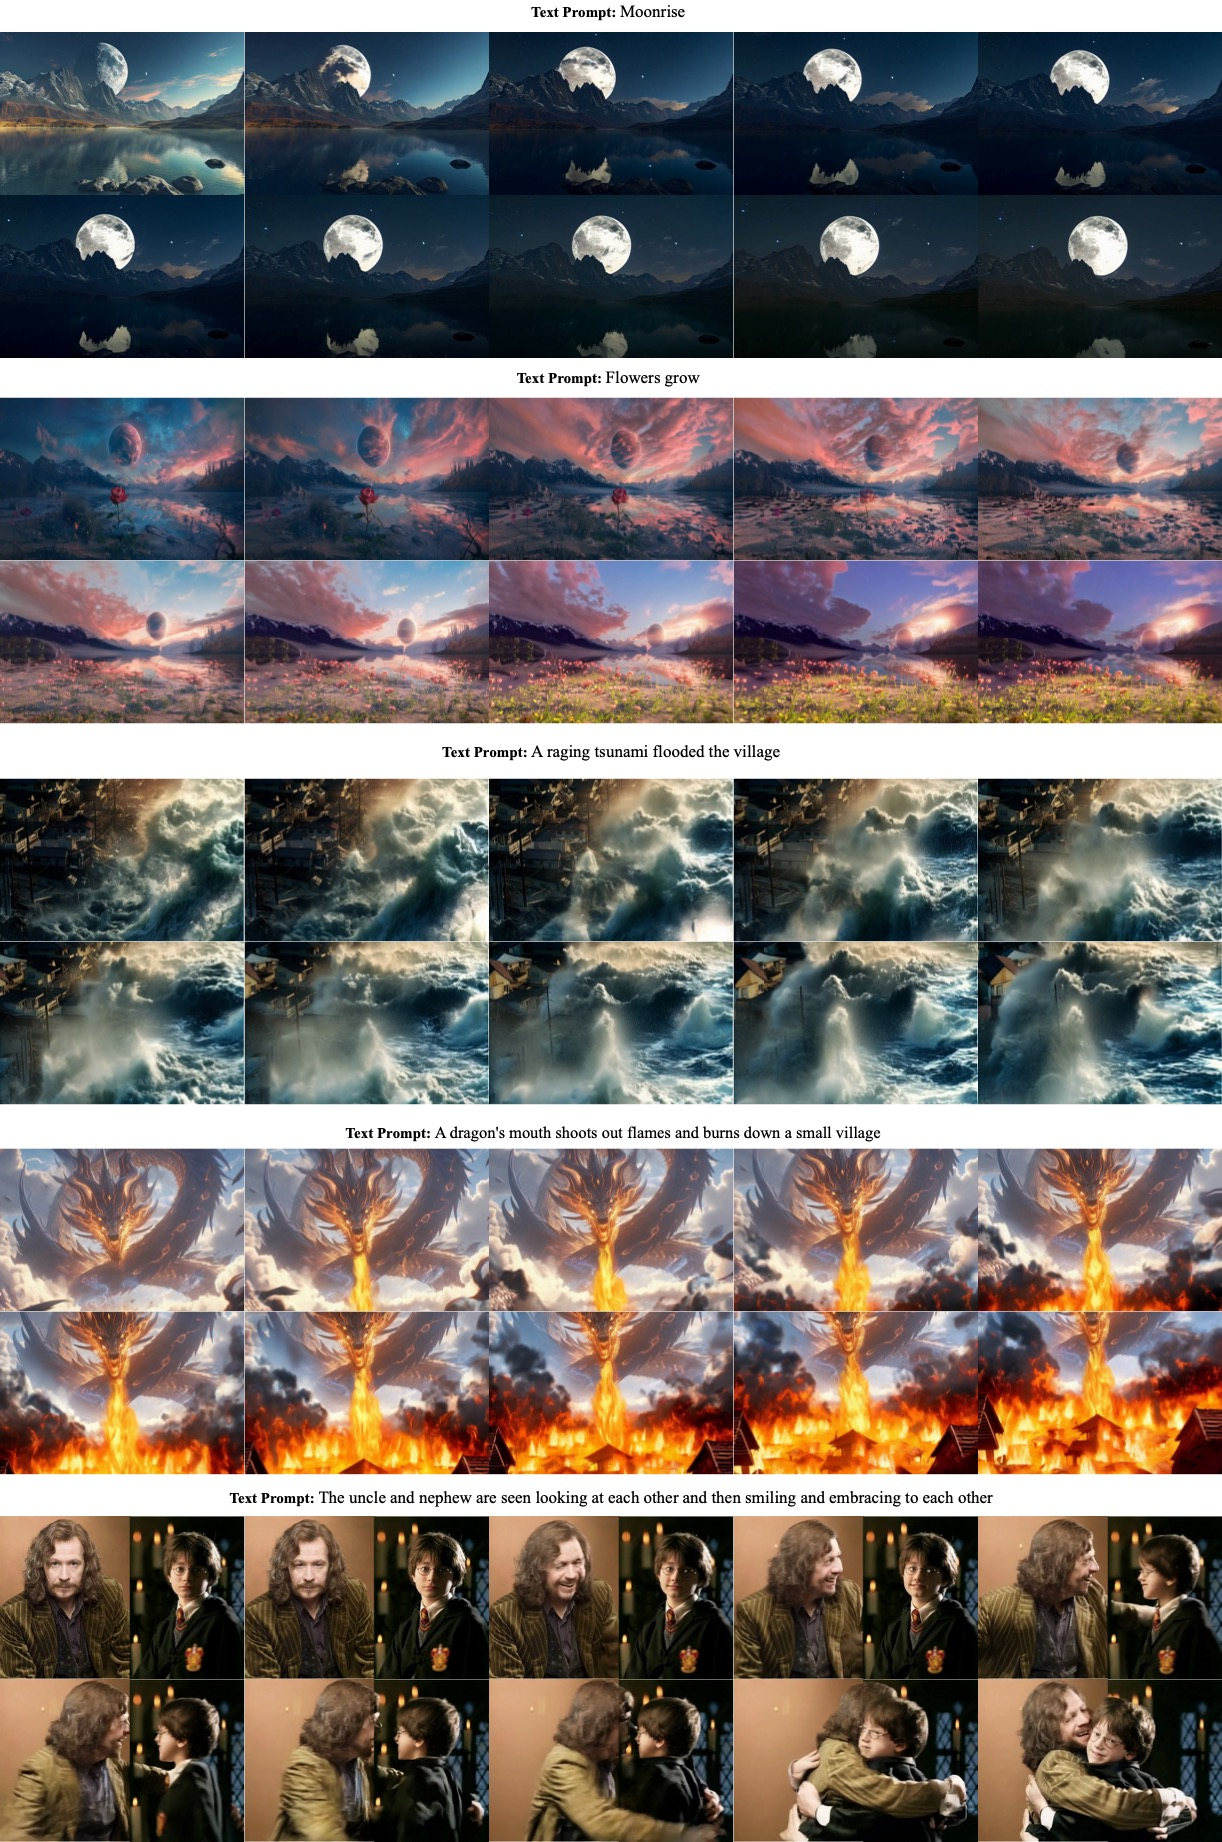
\includegraphics[width=\linewidth]{images/t2v/i2vgood1.jpg}
\end{center}
\caption{Image to video showcases. The displayed prompt will be upsampled before being fed into the model.}
\label{fig:i2vgood1}
\end{figure}

\begin{figure}[ht]
\begin{center}
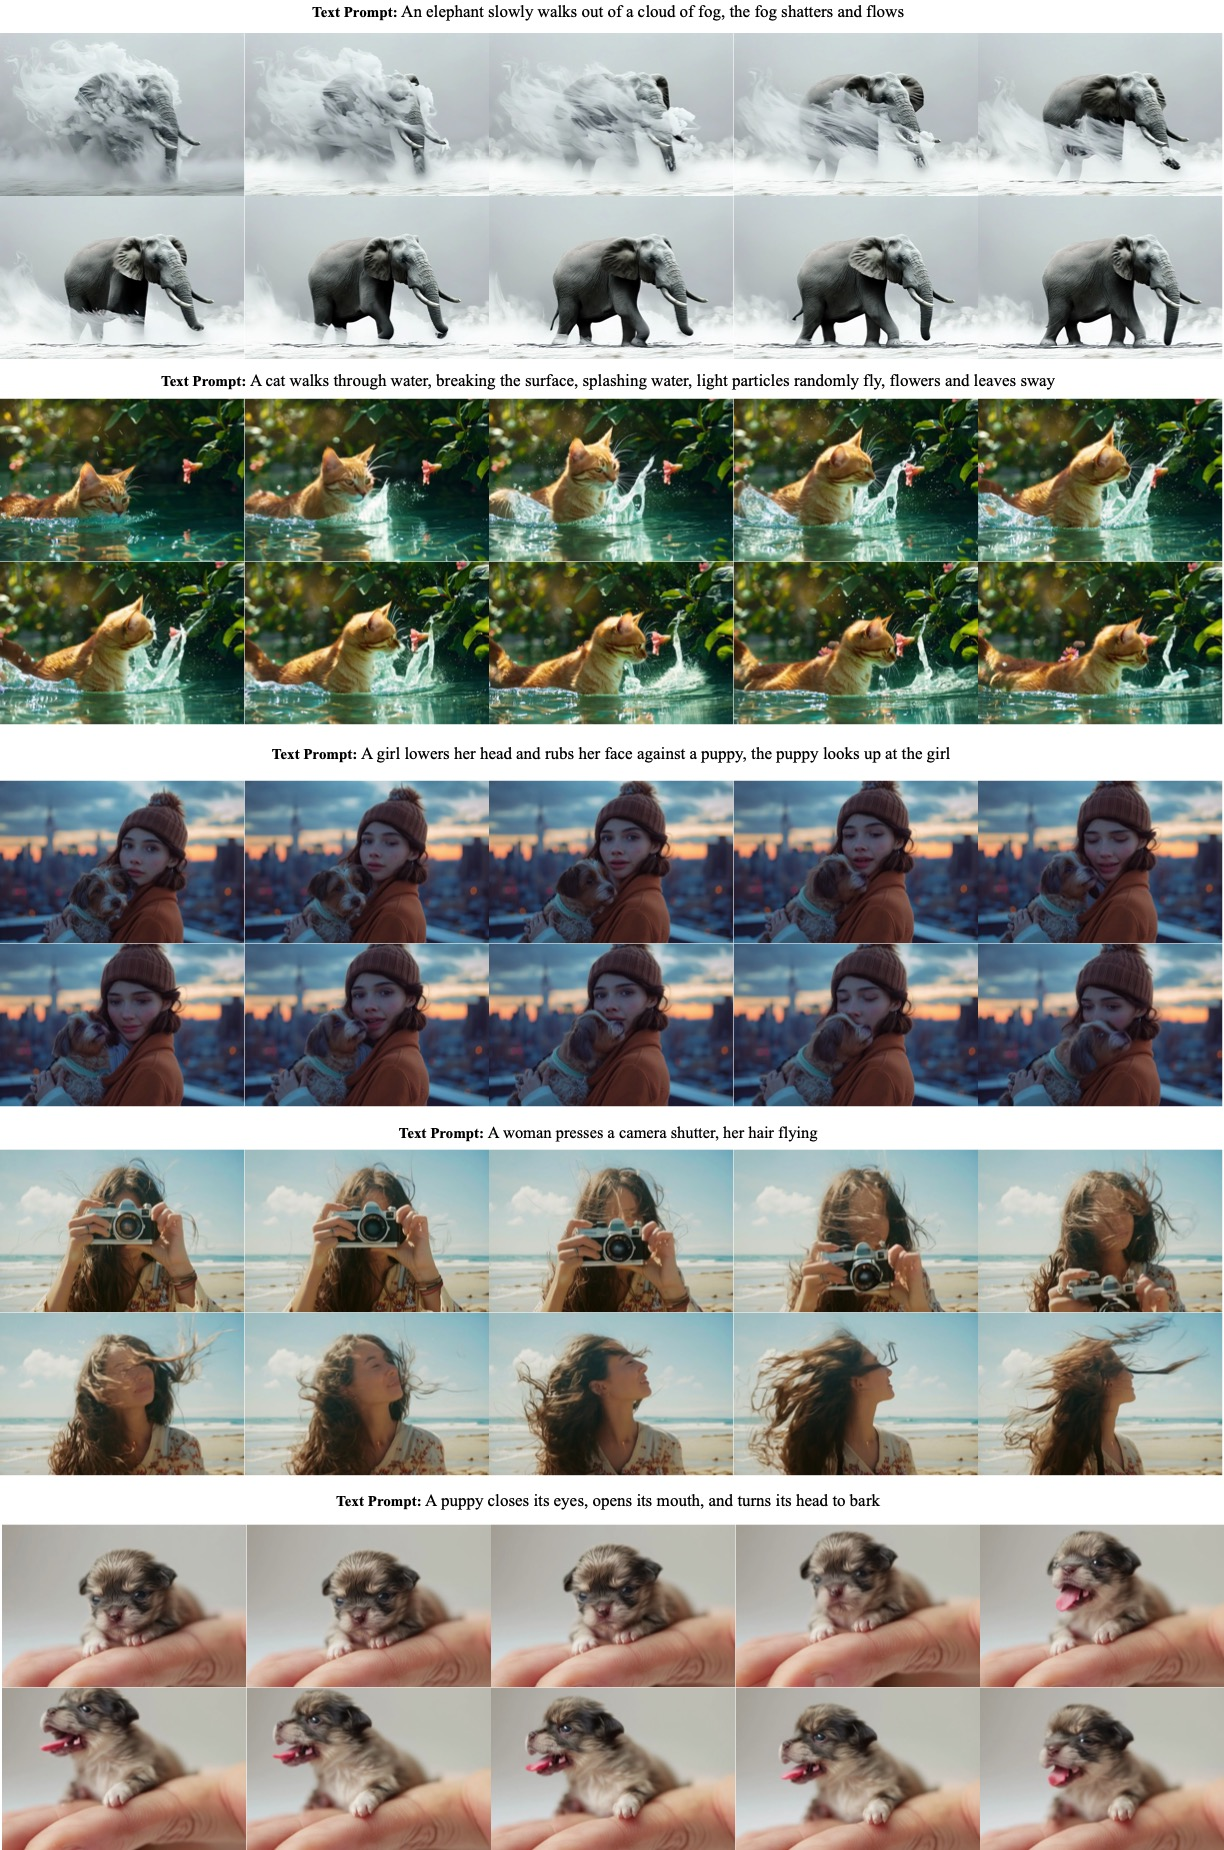
\includegraphics[width=\linewidth]{images/t2v/i2vgood2.jpg}
\end{center}
\caption{Image to video showcases.}
\label{fig:i2vgood2}
\end{figure} \clearpage
\section{Caption Upsampler}
\label{ap:caption_upsampler}
To ensure that text input distribution during inference is as close as possible to the distribution during training, similar to \cite{betker2023improving}, we use a large language model to upsample the user's input during inference, making it more detailed and precise. Finetuned LLM can generate better prompts than zero/few-shot.

For image-to-video, we use the vision language model to upsample the prompt, such as GPT4V, CogVLM\cite{wang2023cogvlm}. 
\begin{promptbox}[Zero-shot prompt for Text Upsampler]
\noindent
\begin{verbatim}
You are part of a team of bots that create videos. You work 
with an assistant bot that will draw anything you say in 
square brackets. For example, outputting \" a beautiful 
morning in the woods with the sun peaking through the 
trees \" will trigger your partner bot to output a video
of a forest morning, as described. You will be prompted 
by people looking to create detailed, amazing videos. 
The way to accomplish this is to take their short prompts
and make them extremely detailed and descriptive.
There are a few rules to follow :
You will only ever output a single video description 
per user request.
When modifications are requested, you should not simply
make the description longer. You should refactor the
entire description to integrate the suggestions.

\end{verbatim}
\end{promptbox}

 \section{Dense Video Caption Data Generation}
\label{ap:video_caption_gen}

In the pipeline for generating video captions, we extract one frame every two seconds for image captioning. Ultimately, we collected 50,000 data points to fine-tune the summary model. Below is the prompt we used for summarization with GPT-4:
\begin{promptbox}[Prompt for GPT-4 Summary]
\noindent
\begin{verbatim}
We extracted several frames from this video and described 
each frame using an image understanding model,  stored 
in the dictionary variable `image_captions: Dict[str: str]`.  
In `image_captions`,  the key is the second at which the image 
appears in the  video,  and the value is a detailed description 
of the image at that moment. Please describe the content of 
this video  in as much detail as possible,  based on the 
information  provided by `image_captions`,  including 
the objects, scenery, animals, characters, and camera 
movements within the video. \n image_captions={new_captions}\n 
You should output your summary directly,  and not mention
variables like `image_captions` in your response. 
Do not include `\\n' and the word 'video' in your response.  
Do not use introductory phrases such as: \"The video 
presents\", \"The video depicts\", \"This video showcases\", 
\"The video captures\" and so on.\n Please start the 
description with the video content directly, such as \"A man
first sits in a chair, then stands up and walks to the 
kitchen....\"\n Do not use phrases like: \"as the video 
progressed\" and \"Throughout the video\".\n Please describe 
the content of the video and the changes that occur, in 
chronological order.\n Please keep the description of this 
video within 100 English words.
\end{verbatim}
\end{promptbox}

 \section{Video Caption Example}
\label{ap:video_caption_example}
Below we present some examples to compare the performance of the Panda-70M video captioning model and our CogVLM2-Caption model:








\begin{figure}[h]
\begin{center}
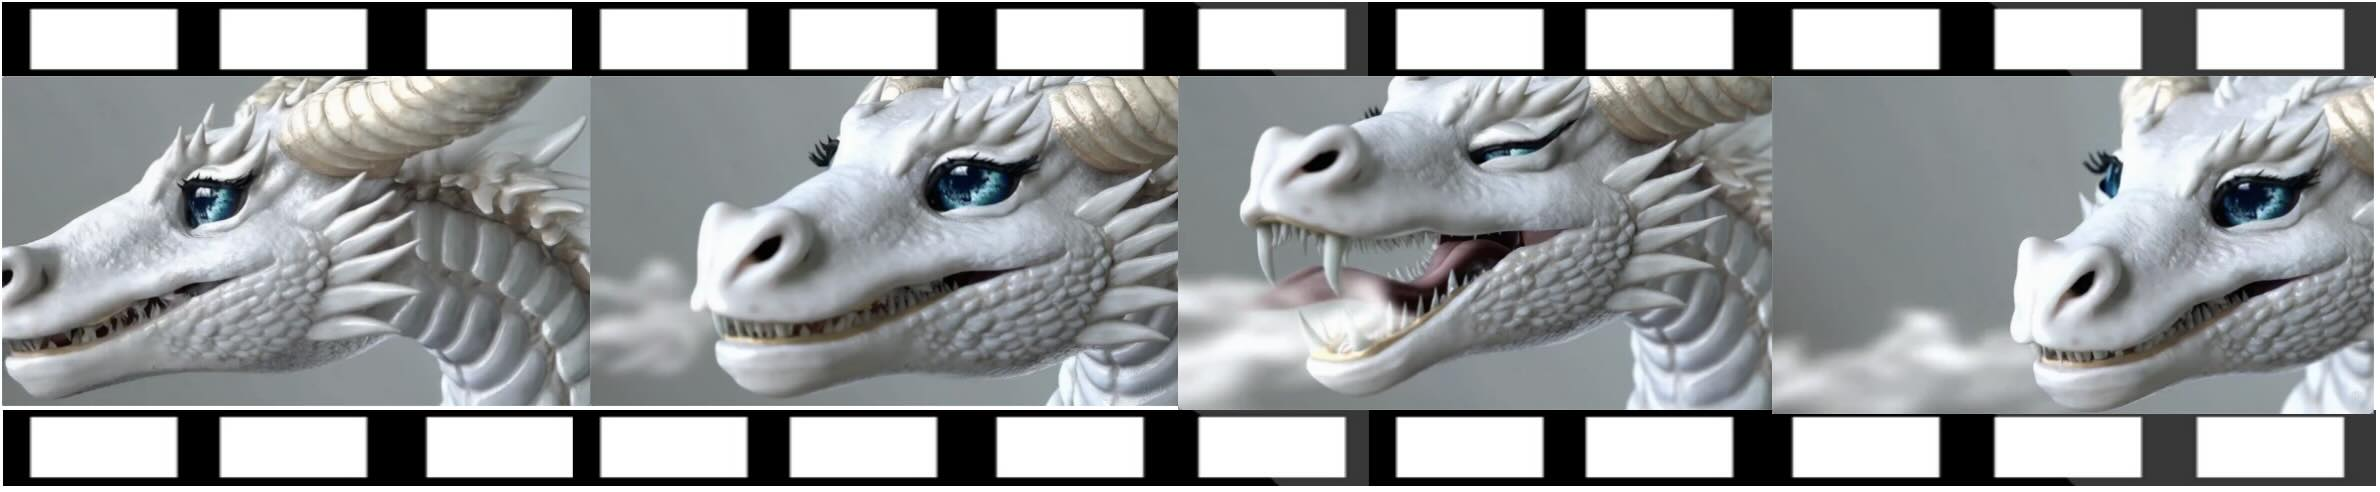
\includegraphics[width=0.9\linewidth]{images/caption_example3.jpg}
\end{center}
\end{figure} \begin{promptbox}[Caption Generated by Panda-70M]
\begin{verbatim}
A close up of a white dragon with blue eyes.
\end{verbatim}
\end{promptbox}
\begin{promptbox}[Caption Generated by CogVLM2-Caption]
\begin{verbatim}
A meticulously crafted white dragon with a serene expression 
and piercing blue eyes is showcased in various close-ups, its 
scales detailed with golden highlights. Initially, the dragon's
horns are curved back, but as time passes, they change to 
spiraling gold, adding elegance. The creature's demeanor shifts 
from tranquil majesty to a more formidable presence, with its 
mouth agape revealing sharp teeth at times. Its expressions 
alternate between calmness and fierce determination, 
maintaining an air of mythical serenity throughout. The 
consistent neutral background focuses attention on the dragon's
textured features and expressive eyes.
\end{verbatim}
\end{promptbox}


\begin{figure}[h]
\begin{center}
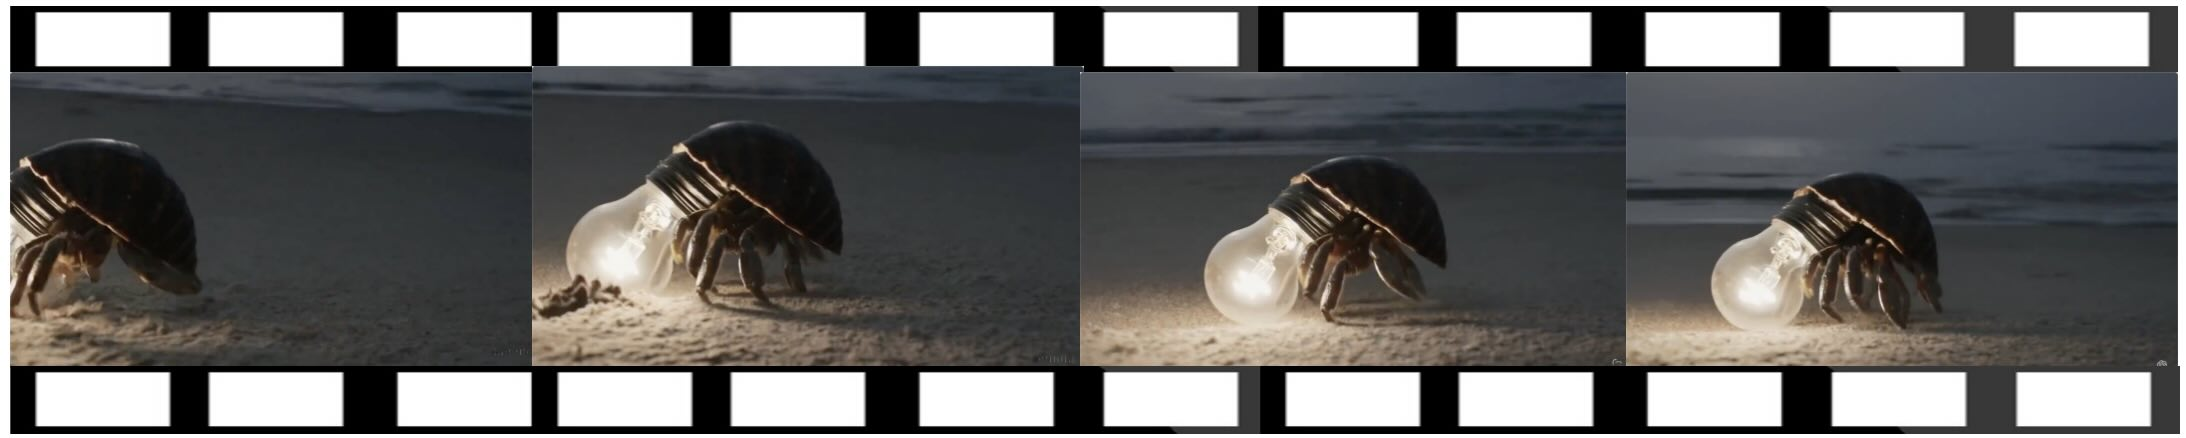
\includegraphics[width=0.9\linewidth]{images/caption_example4.jpg}
\end{center}
\end{figure} \begin{promptbox}[Caption Generated by Panda-70M]
\begin{verbatim}
A crab is walking on the beach with a light bulb on its back.
\end{verbatim}
\end{promptbox}
\begin{promptbox}[Caption Generated by CogVLM2-Caption]
\begin{verbatim}
A hermit crab with a dark, glossy shell and reddish-brown legs
is seen carrying an illuminated light bulb on its back across 
the sandy terrain of a beach at night. The scene transitions 
from a soft glow to a more pronounced illumination as the crab
moves, highlighting its delicate limbs against the smooth sand
and tranquil sea backdrop. This surreal tableau blends natural
beauty with human ingenuity, creating a serene yet whimsical 
atmosphere that emphasizes the crab's unique adaptation and the
contrast between nature and technology in this quiet nocturnal
setting.
\end{verbatim}
\end{promptbox}


\begin{figure}[h]
\begin{center}
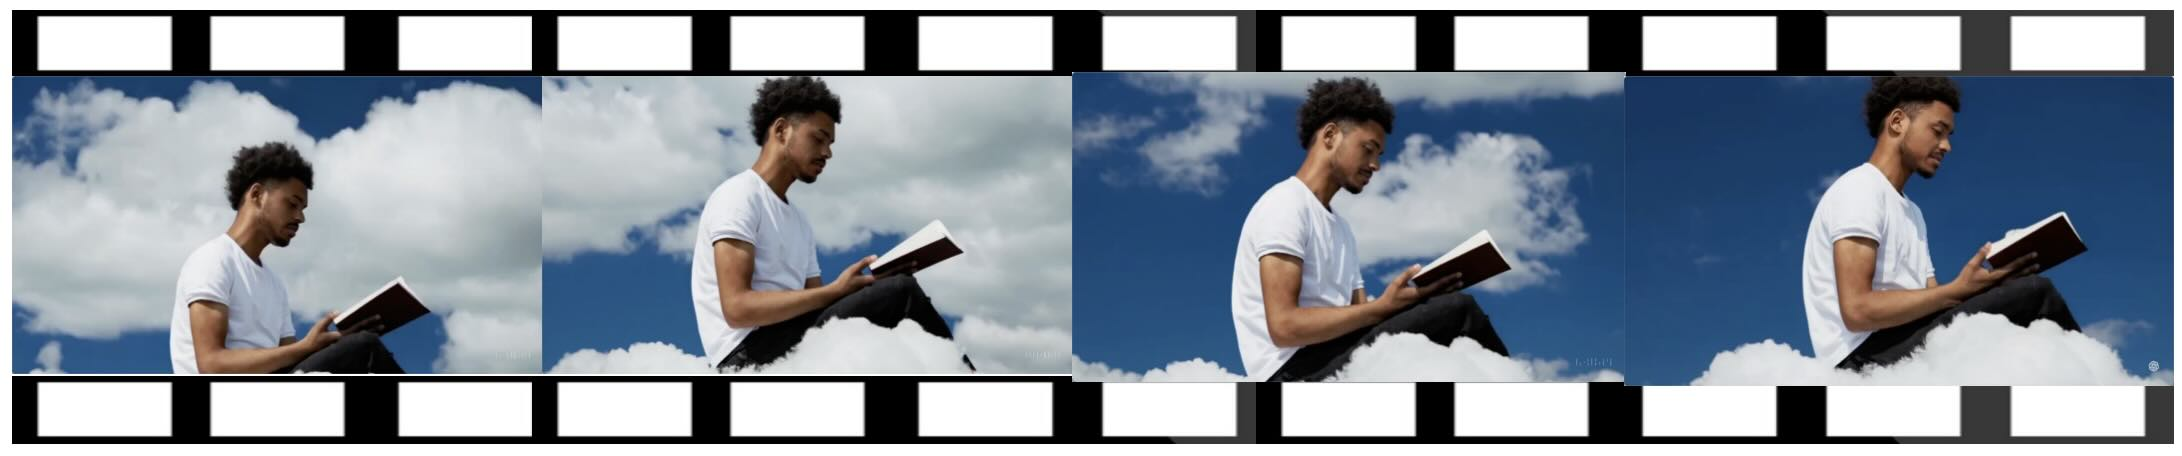
\includegraphics[width=0.9\linewidth]{images/caption_example5.jpg}
\end{center}
\end{figure} \begin{promptbox}[Caption Generated by Panda-70M]
\begin{verbatim}
A young black man is sitting on a cloud and reading a book 
with a blue sky in the background.
\end{verbatim}
\end{promptbox}
\begin{promptbox}[Caption Generated by CogVLM2-Caption]
\begin{verbatim}
A young Black man with an afro hairstyle and a neatly trimmed 
beard is seen sitting cross-legged on fluffy white clouds, 
deeply engrossed in reading a book with a red cover. He wears 
a plain white T-shirt and dark pants against a vivid blue sky 
dotted with cumulus clouds. Throughout the scenes, his 
expression remains one of deep concentration and peaceful 
contemplation, highlighting a moment of intellectual pursuit 
amidst nature's grandeur. The imagery suggests a serene 
atmosphere that emphasizes solitude and introspection, with no 
other people or objects around him.
\end{verbatim}
\end{promptbox}





%
 \clearpage
\section{Video to Video via CogVideoX and CogVLM2-Caption}
\label{ap:v2v}

In this section, we present several examples of video-to-video generation using CogVideoX and CogVLM2-Caption. Specifically, we first input the original video into CogVLM2-Caption to obtain the video's caption, and then feed this caption into the CogVideoX model to generate a new video. From the examples below, it can be seen that our pipeline achieves a high degree of fidelity to the original video:

\begin{figure}[h]
\begin{center}
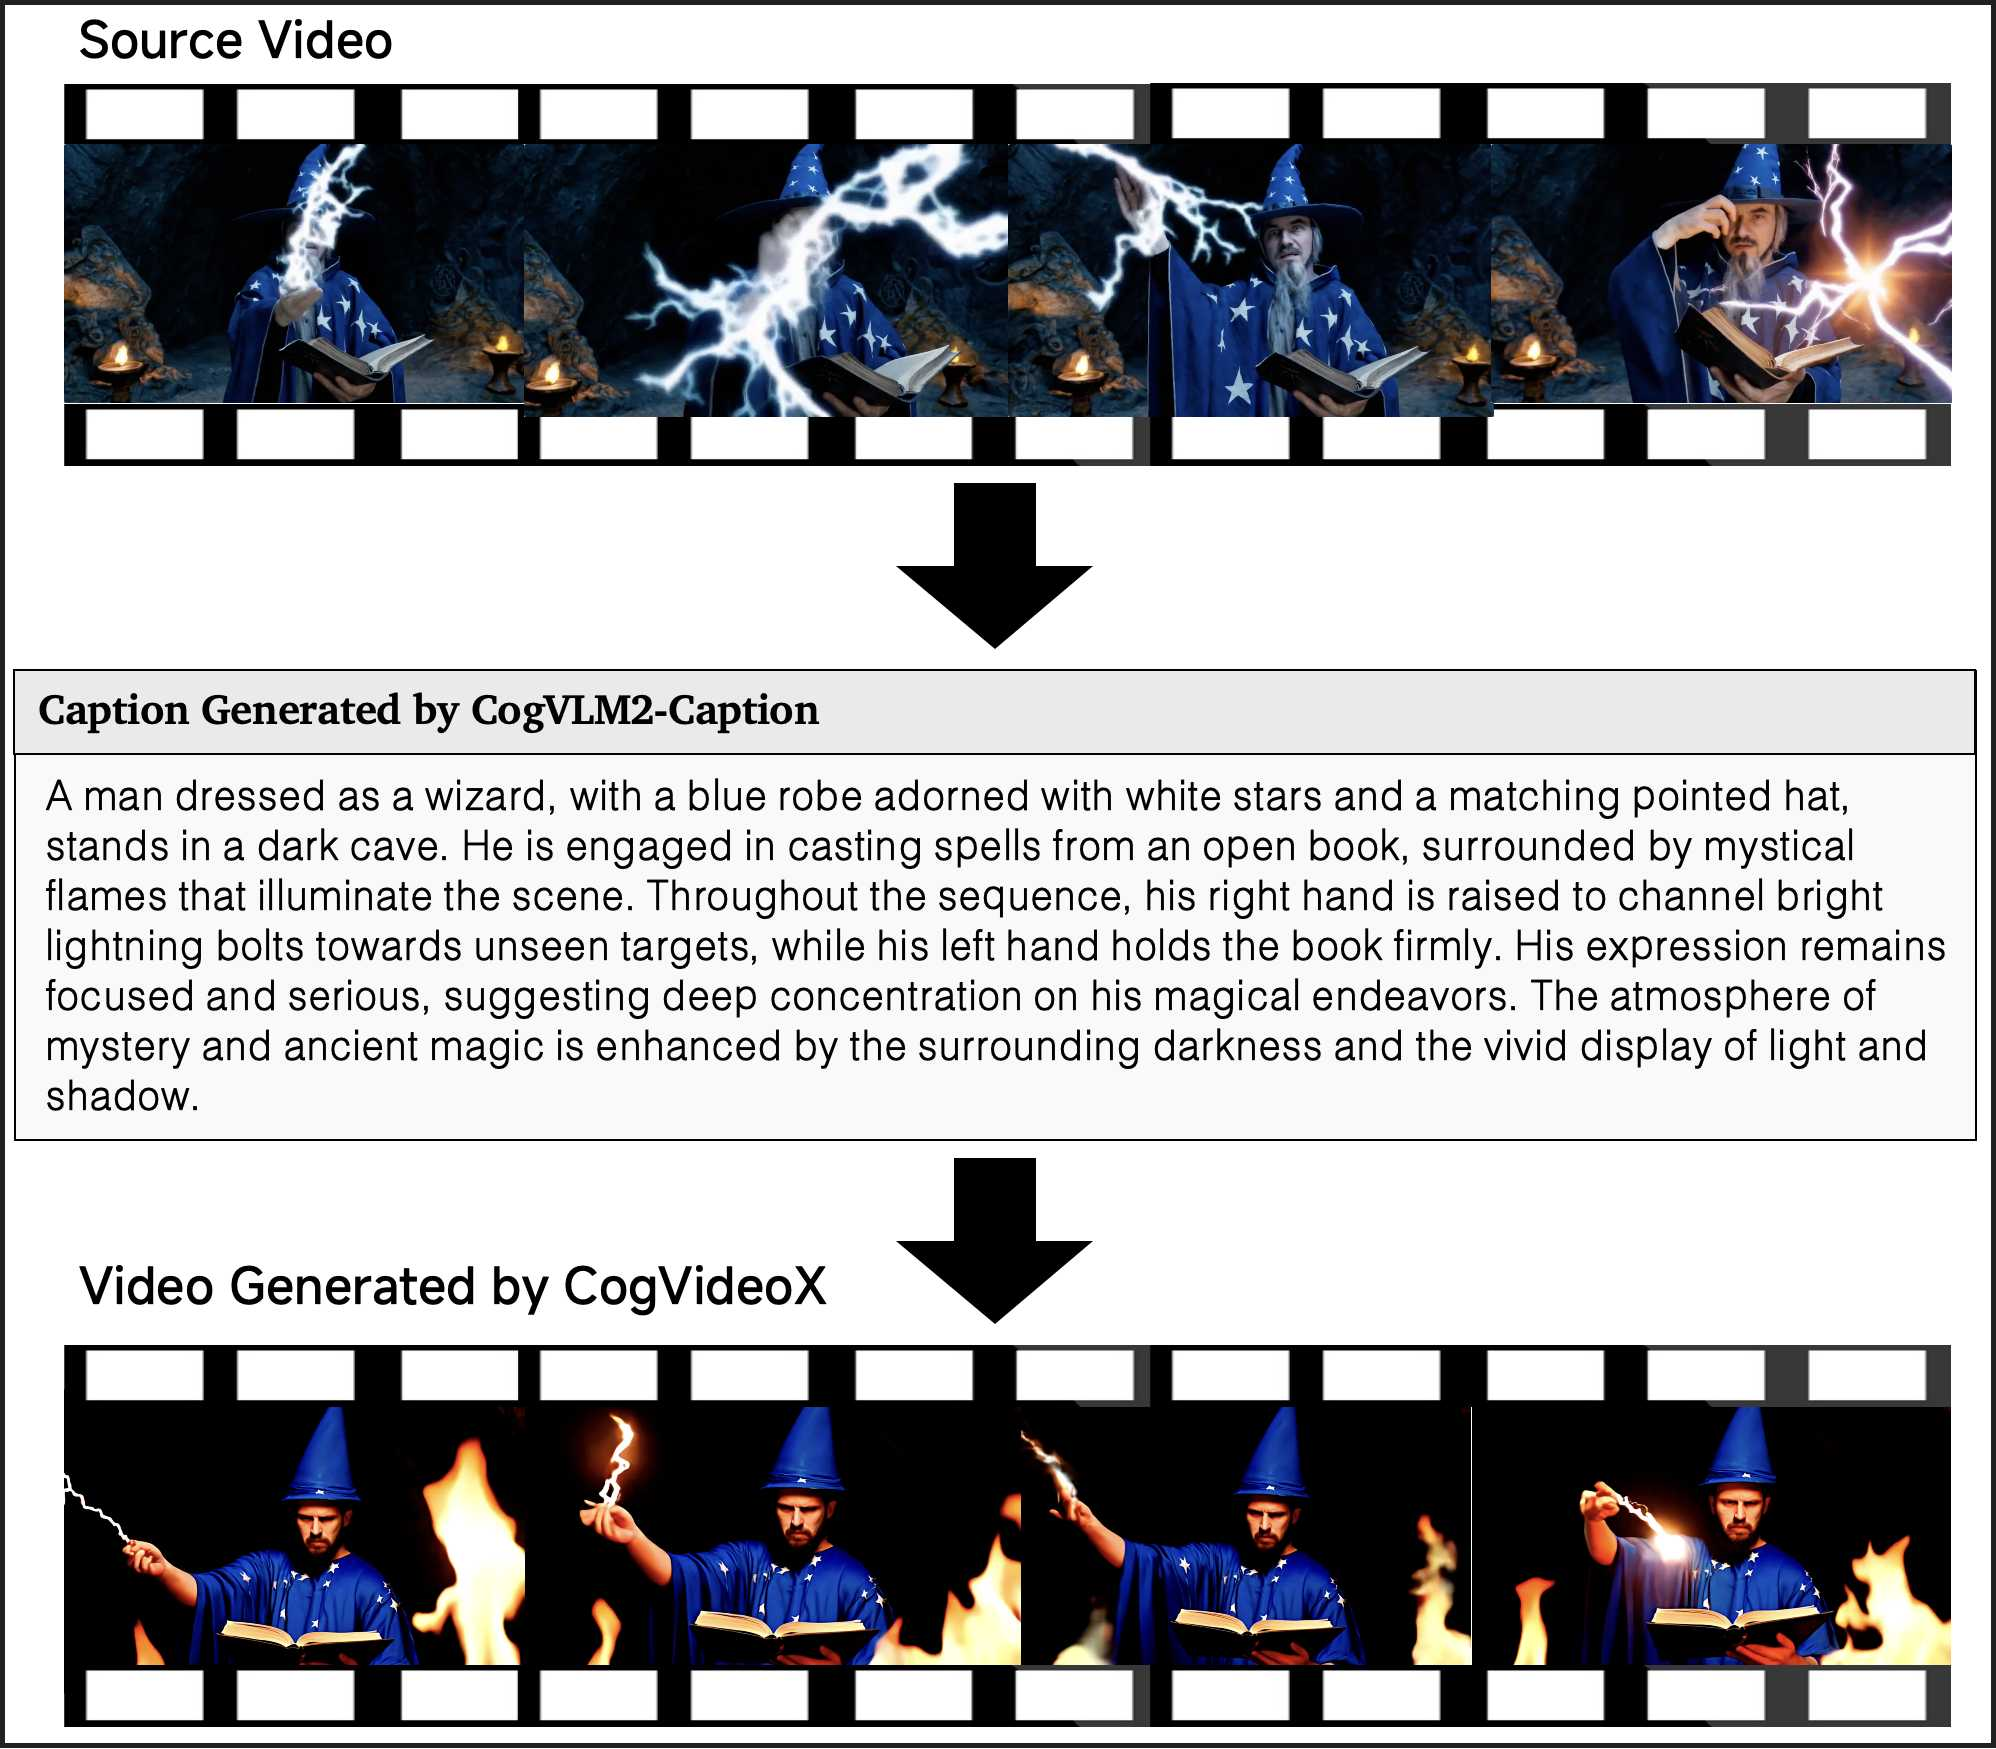
\includegraphics[width=0.9\linewidth]{images/v2v/v2v_1.jpg}
\end{center}
\end{figure}
 \begin{figure}[h]
\begin{center}
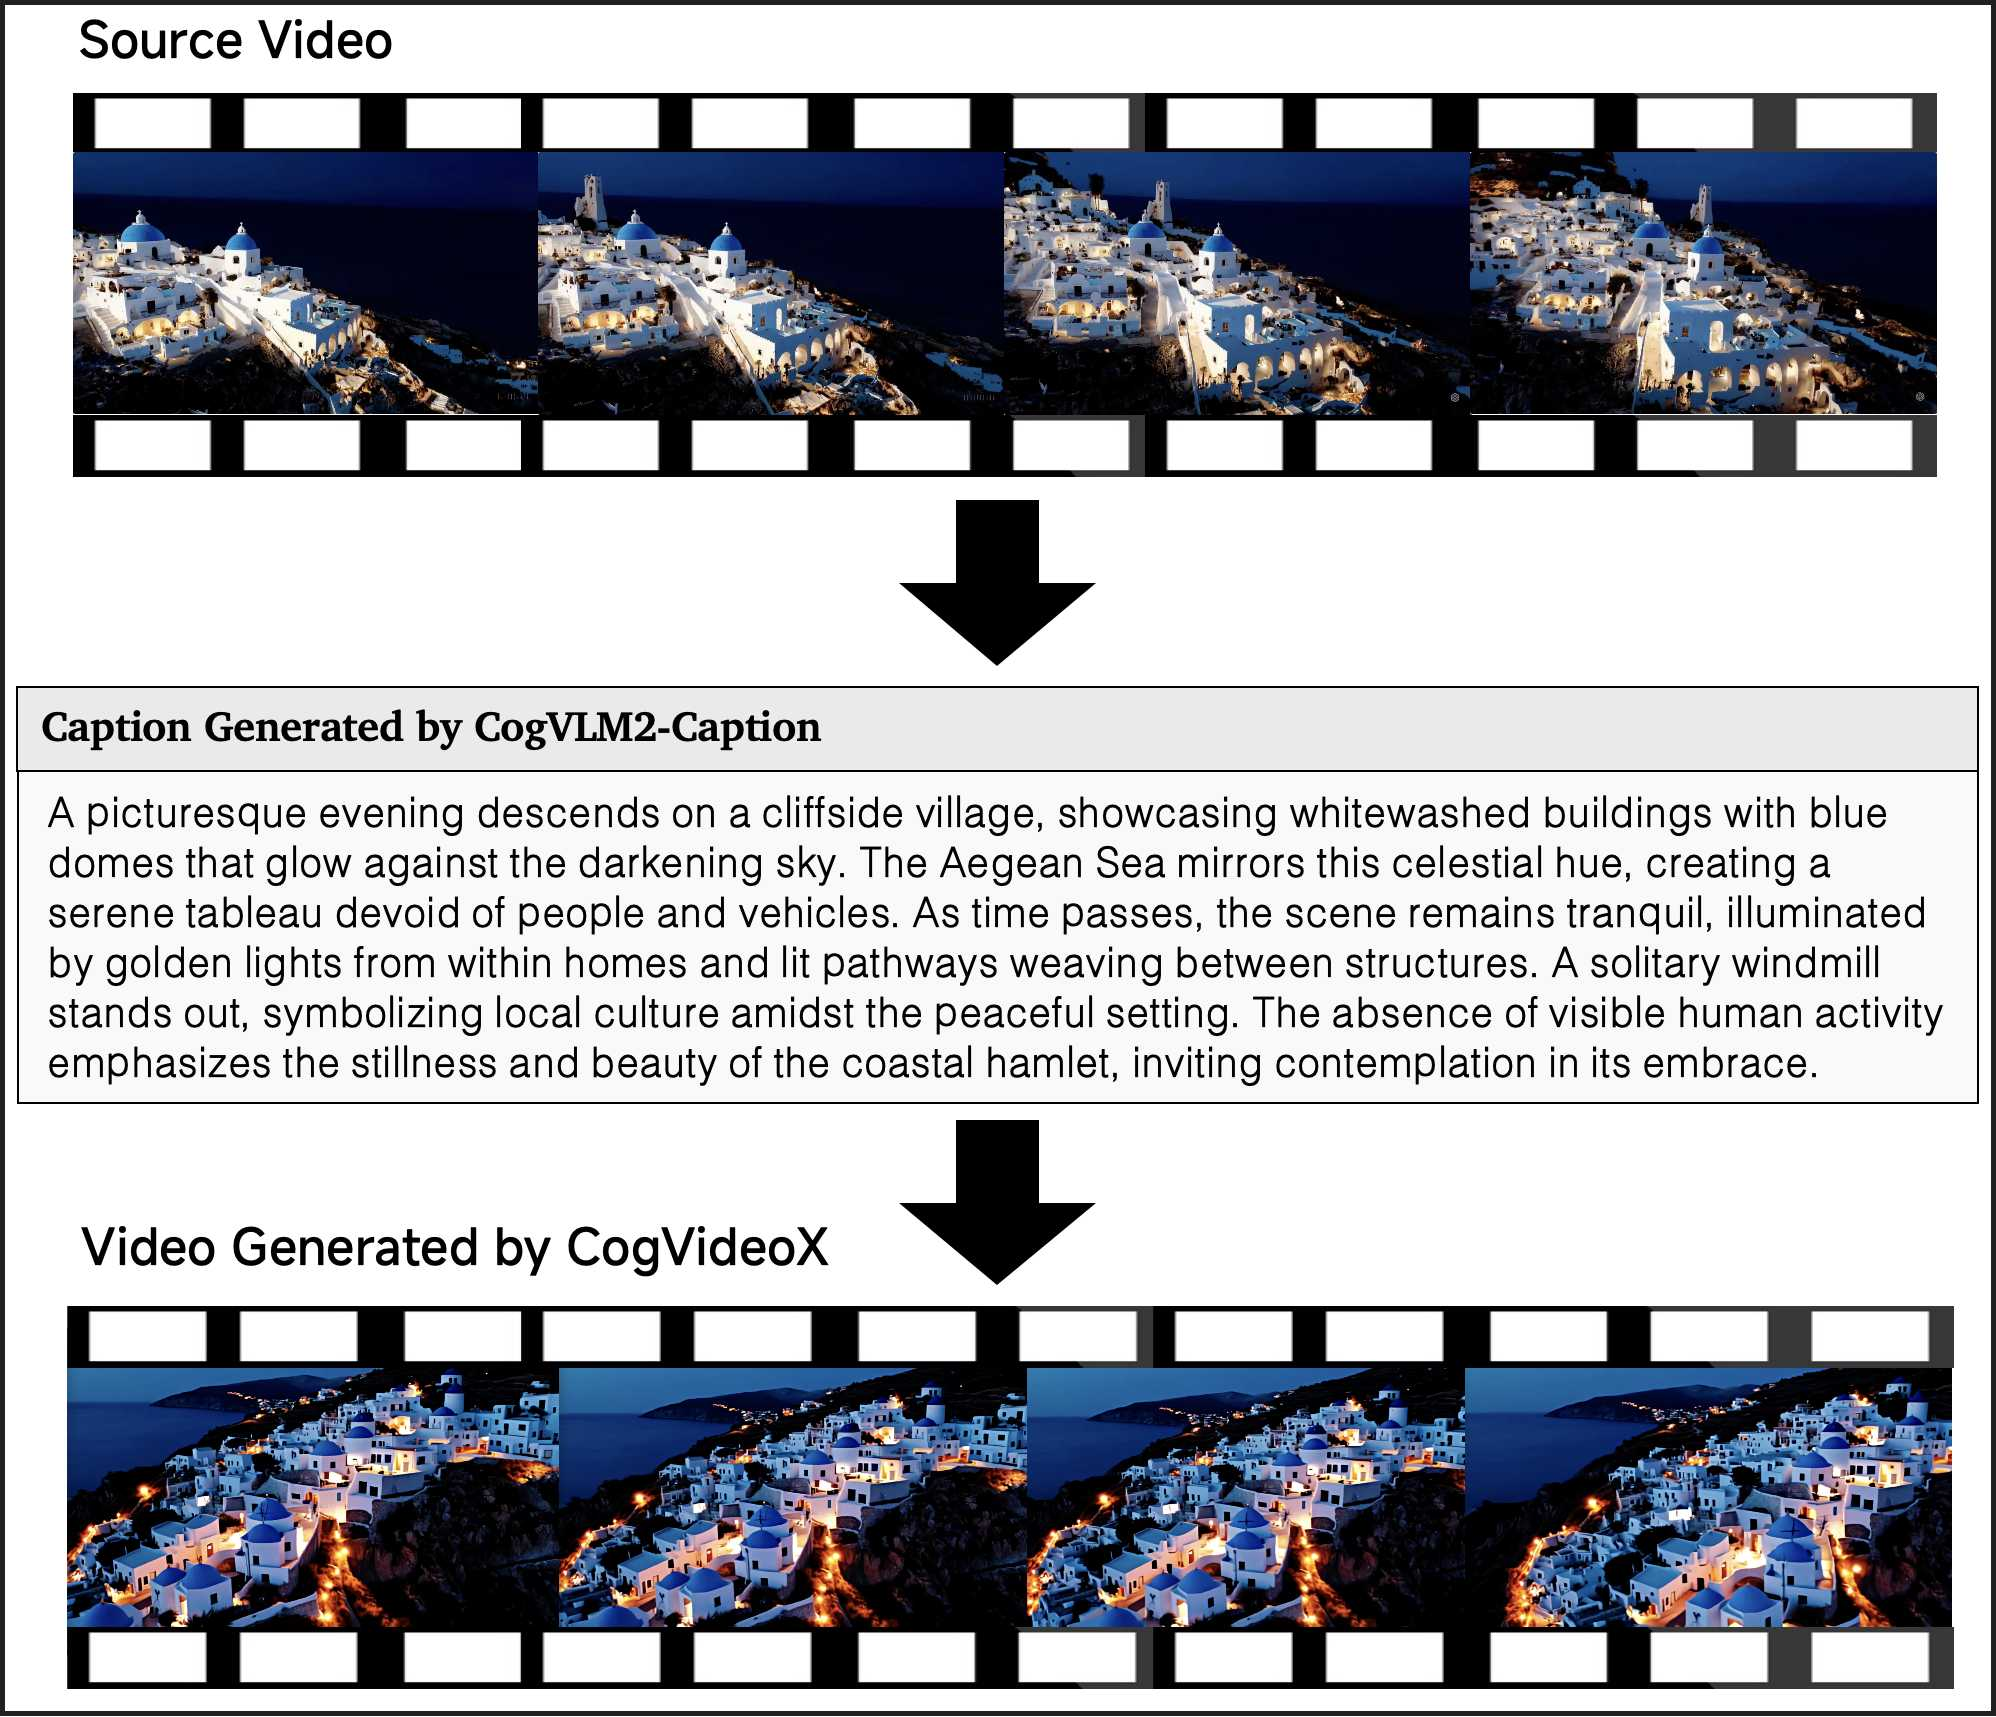
\includegraphics[width=0.9\linewidth]{images/v2v/v2v_2.jpg}
\end{center}
\end{figure}
 \begin{figure}[h]
\begin{center}
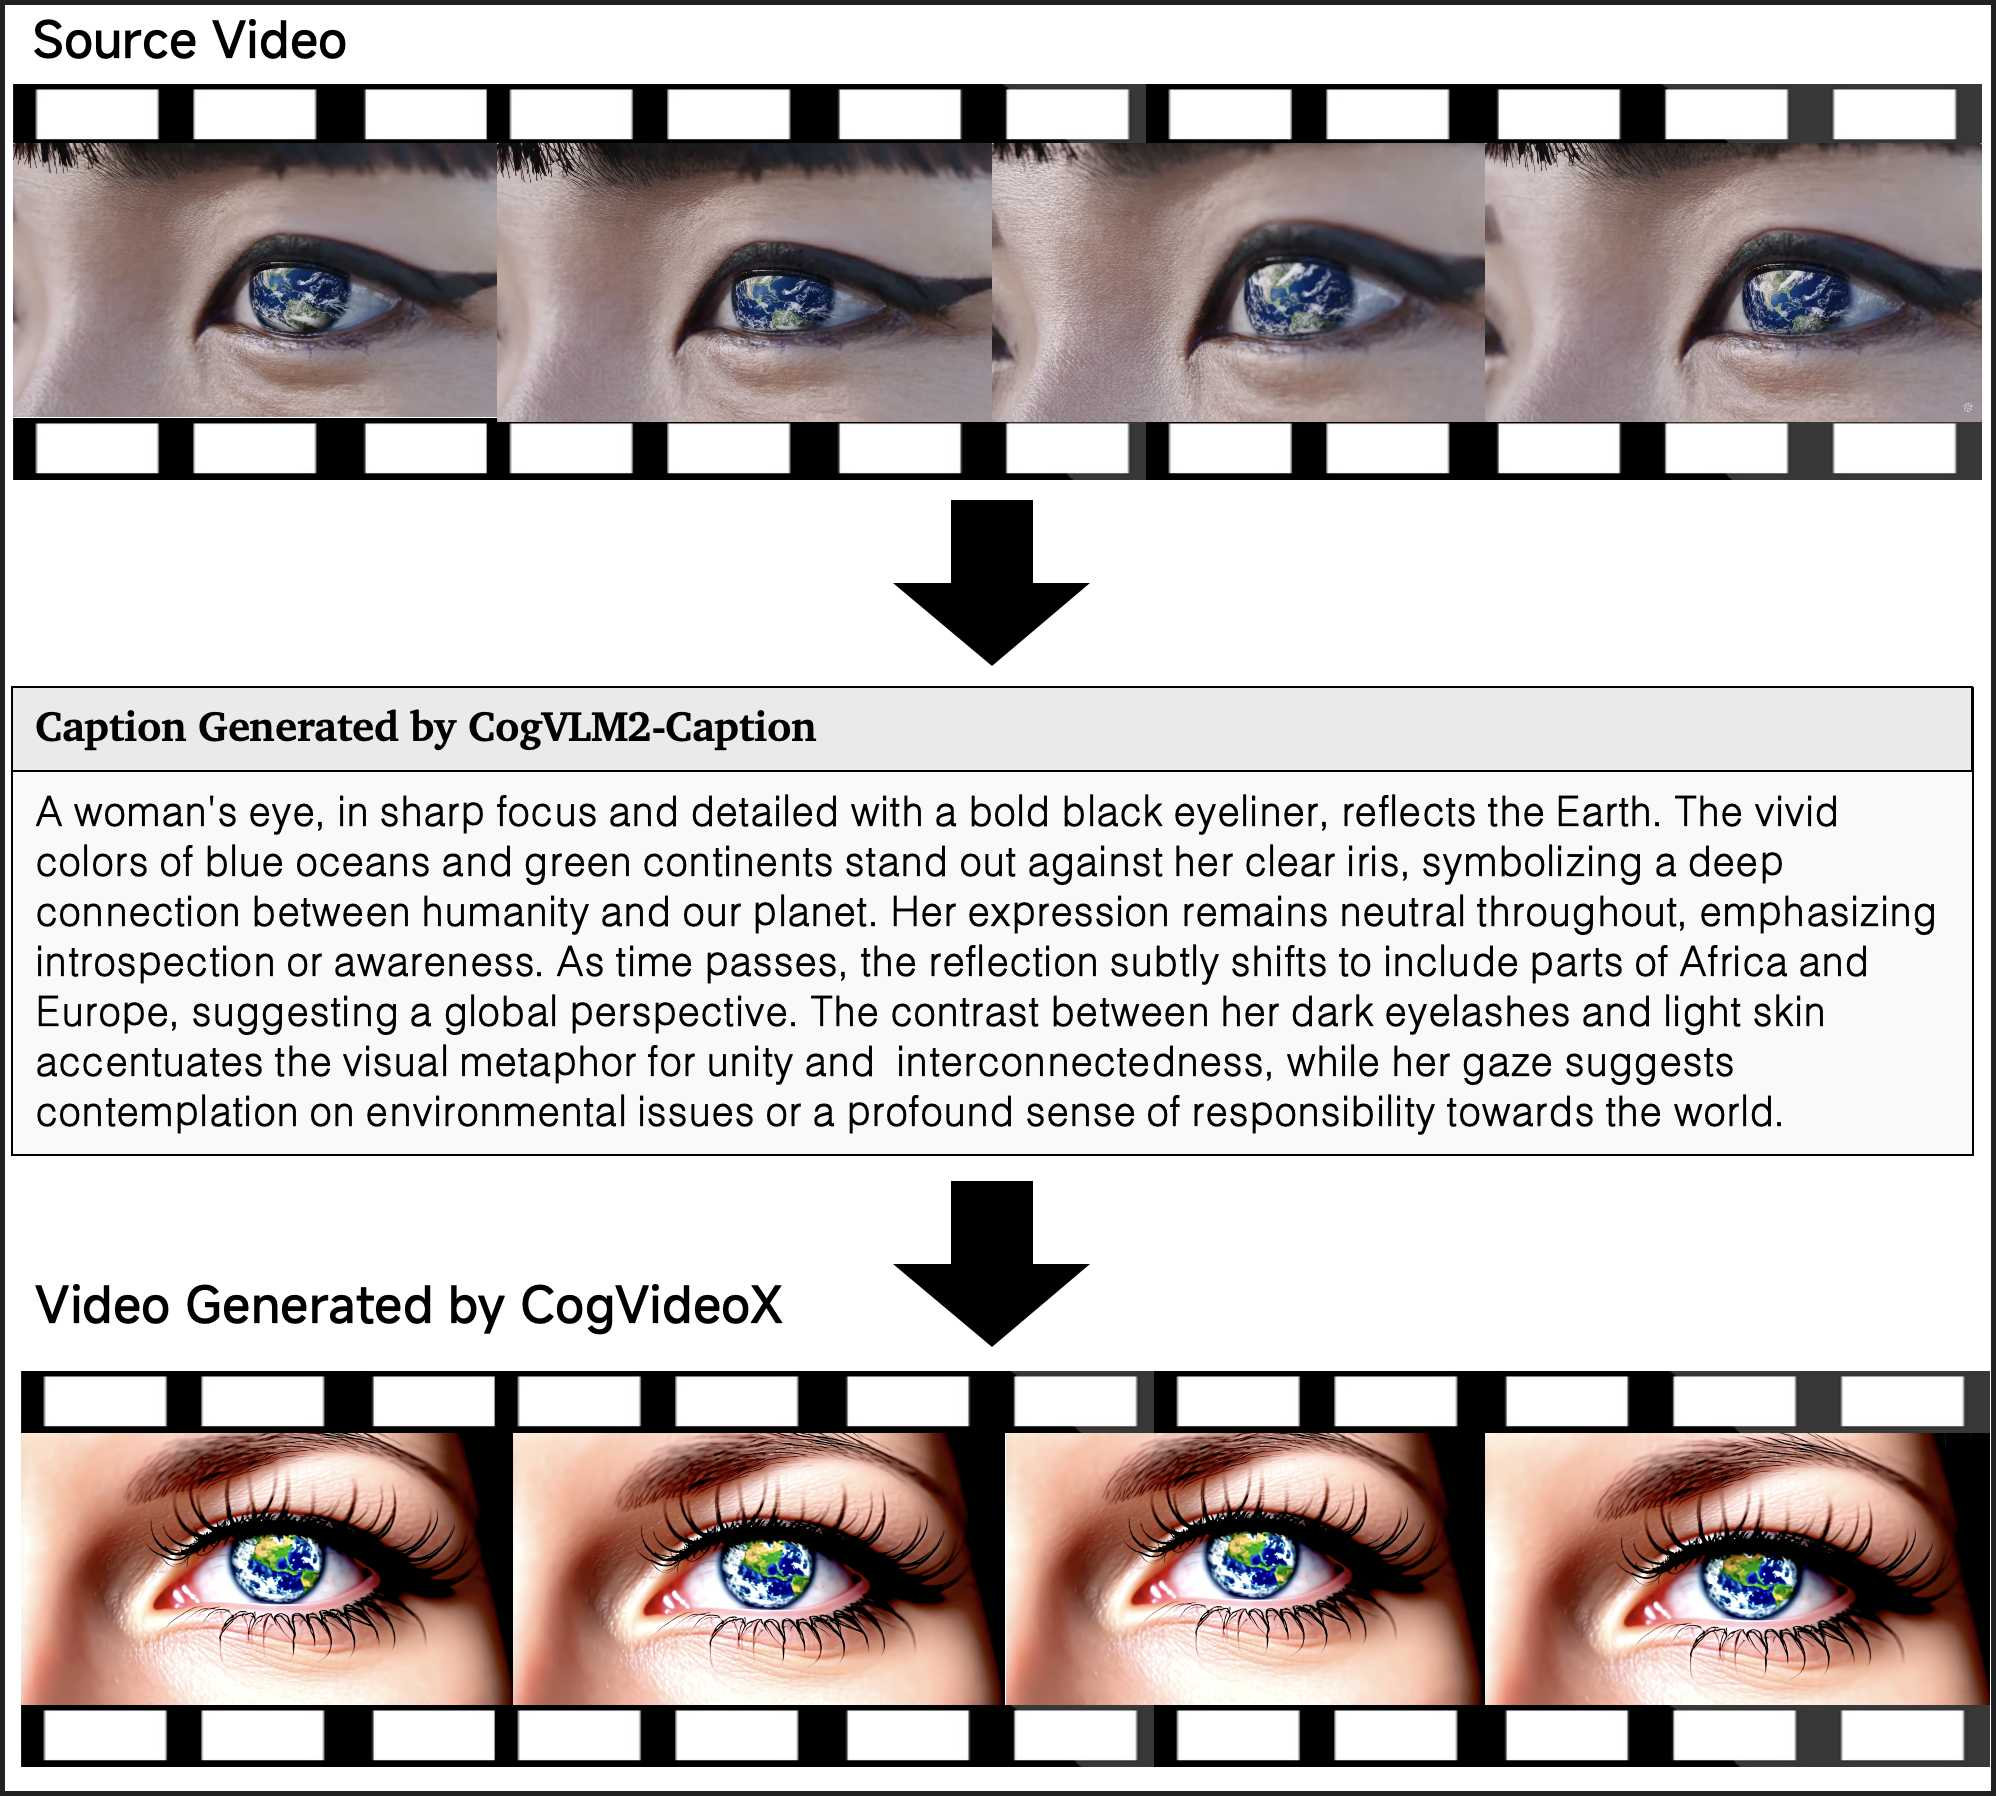
\includegraphics[width=0.9\linewidth]{images/v2v/v2v_3.jpg}
\end{center}
\end{figure}
  \clearpage
\section{Human Evaluation Details}\label{sec:human_evalution}

Sensory Quality: This part focuses mainly on the perceptual quality of videos, including subject consistency, frame continuity, and stability.

\begin{table}[h]
\centering
\caption{Sensory Quality Evaluation Criteria.}
\label{sample-table}
\small

\begin{tabular}{cp{11cm}}
\toprule

\textbf{Score} & \textbf{Evaluation Criteria} \\
\midrule
1  & High sensory quality: 1. The appearance and morphological features of objects in the video are completely consistent 2. High picture stability, maintaining high resolution consistently 3. Overall composition/color/boundaries match reality 4. The picture is visually appealing \\
\midrule
0.5  & Average sensory quality: 1. The appearance and morphological features of objects in the video are at least 80\% consistent 2. Moderate picture stability, with only 50\% of the frames maintaining high resolution 3. Overall composition/color/boundaries match reality by at least 70\% 4. The picture has some visual appeal \\
\midrule
0  & Poor sensory quality: large inconsistencies in appearance and morphology, low video resolution, and composition/layout not matching reality \\

\bottomrule
\end{tabular}
\end{table}

Instruction Following: This part focuses on whether the generated video aligns with the prompt, including the accuracy of the subject, quantity, elements, and details.

\begin{table}[h]
\centering
\caption{Instruction Following Evaluation Criteria.}
\label{sample-table}
\small

\begin{tabular}{cp{11cm}}
\toprule

\textbf{Score} & \textbf{Evaluation Criteria} \\
\midrule
1  & 100\% follow the text instruction requirements, including but not limited to: elements completely correct, quantity requirements consistent, elements complete, features accurate, etc. \\
\midrule
0.5  & 100\% follow the text instruction requirements, but the implementation has minor flaws such as distorted main subjects or inaccurate features. \\
\midrule
0  & Does not 100\% follow the text instruction requirements, with any of the following issues:  1. Generated elements are inaccurate  2. Quantity is incorrect  3. Elements are incomplete  4. Features are inaccurate \\
\bottomrule
\end{tabular}
\end{table}



Physics Simulation: This part focuses on whether the model can adhere to the objective law of the physical world, such as the lighting effect, interactions between different objects, and the realism of fluid dynamics. 


\begin{table}[h]
\centering
\caption{Physics Simulation Evaluation Criteria.}
\label{sample-table}
\small

\begin{tabular}{cp{11cm}}
\toprule

\textbf{Score} & \textbf{Evaluation Criteria} \\
\midrule
1  & Good physical realism simulation capability, can achieve: 1. Real-time tracking 2. Good action understanding, ensuring dynamic realism of entities 3. Realistic lighting and shadow effects, high interaction fidelity 4. Accurate simulation of fluid motion \\
\midrule
0.5  & Average physical realism simulation capability, with some degradation in real-time tracking, dynamic realism, lighting and shadow effects, and fluid motion simulation. Issues include: 1. Slightly unnatural transitions in dynamic effects, with some discontinuities 2. Lighting and shadow effects not matching reality 3. Distorted interactions between objects 4. Floating fluid motion, not matching reality \\
\midrule
0  & Poor physical realism simulation capability, results do not match reality, obviously fake \\

\bottomrule
\end{tabular}
\end{table}



\newpage
Cover Quality: This part mainly focuses on metrics that can be assessed from single-frame images, including aesthetic quality, clarity, and fidelity.

\begin{table}[h]
\centering
\caption{Cover Quality Evaluation Criteria.}
\label{sample-table}
\small

\begin{tabular}{cp{11cm}}
\toprule

\textbf{Score} & \textbf{Evaluation Criteria} \\
\midrule
1 & Image is clear, subject is obvious, display is complete, color tone is normal. \\
\midrule
0.5 & Image quality is average. The subject is relatively complete, color tone is normal. \\
\midrule
0 & Cover image resolution is low, image is blurry. \\

\bottomrule
\end{tabular}
\end{table}
 }

\end{document}
